\documentclass[doublespace]{umassthesis}
\usepackage{courier}
\usepackage{epsfig}
%\usepackage{ulem}
\usepackage{enumitem}
\usepackage{graphicx}
\graphicspath{ {figure/} } 
\usepackage{caption}
\usepackage{subcaption}
%\usepackage{subcaption}
%\usepackage{subfigure}

\usepackage{amssymb}
\usepackage{amsmath}
\usepackage{amsfonts}
\usepackage{color}
\usepackage{hhline}
\usepackage{multirow}

\usepackage{algorithm}
\usepackage{algpseudocode}
%\usepackage{hyperref}
\usepackage[T1]{fontenc}
\usepackage[authoryear,round]{natbib}
%\bibliographystyle{umthesis}
\bibliographystyle{plainnat}
%\setcitestyle{authoryear,open={(},close={)}}

\usepackage{xspace}
\usepackage{amsthm}

\theoremstyle{definition}
\newtheorem{definition}{Definition}
[section]

\DeclareMathOperator*{\argmax}{argmax}

\newcommand{\mylistbegin}{
  \begin{list}{$\bullet$}
   {
     \setlength{\itemsep}{-2pt}
     %\setlength{\parsep}{0pt}
     %\setlength{\topsep}{0pt}
     %\setlength{\partopsep}{0pt}
     \setlength{\leftmargin}{1em}
     \setlength{\labelwidth}{1em}
     \setlength{\labelsep}{0.5em} } }

\newcommand{\mylistend}{
   \end{list}  }
\newcommand{\eg}{\textit{e.g.}}
\newcommand{\xeg}{\textit{E.g.}}
\newcommand{\ie}{\textit{i.e.}}
\newcommand{\etc}{\textit{etc.}}
\newcommand{\etal}{\textit{et al.}}
\newcommand{\wrt}{\textit{w.r.t.}}
\newcommand{\header}[1]{{\flushleft \textbf{#1}}}
\newcommand{\sheader}[1]{{\flushleft \textit{#1}}}

\newcommand{\floor}[1]{\lfloor #1 \rfloor}
\newcommand{\ceil}[1]{\lceil #1 \rceil}


% data
\newcommand{\DQF}{QF13\xspace}
\newcommand{\DFWS}{FWS14\xspace}

% models
\newcommand{\QF}{QF\xspace}
\newcommand{\QFI}{QFI\xspace}
\newcommand{\QFJ}{QFJ\xspace}
\newcommand{\QDM}{QDM\xspace}
\newcommand{\PLSA}{pLSA\xspace}
\newcommand{\LDA}{LDA\xspace}

\newcommand{\MLE}{MLE\xspace}
\newcommand{\EUM}{EUM\xspace}
\newcommand{\EUMab}[2]{$EU\!M_{{#1},{#2}}$}

%measures
\newcommand{\TP}{$T\!P$\xspace}
\newcommand{\TR}{$T\!R$\xspace}
\newcommand{\TF}{$T\!F$\xspace}
\newcommand{\PP}{$P\!P$\xspace}
\newcommand{\PR}{$P\!R$\xspace}
\newcommand{\PF}{$P\!F$\xspace}
\newcommand{\PRFab}[2]{$P\!R\!F_{\alpha={#1},\beta={#2}}$}
\newcommand{\PRF}{$P\!R\!F_{\alpha,\beta}$\xspace}
\newcommand{\PRFe}{P\!R\!F_{\alpha,\beta}} % for equation

\newcommand{\bx}{\boldsymbol{x}}
\newcommand{\bw}{\boldsymbol{w}}
\newcommand{\bW}{\boldsymbol{W}}
\newcommand{\bfn}{\boldsymbol{f}}
\newcommand{\blambda}{\boldsymbol{\lambda}}
\newcommand{\btheta}{\boldsymbol{\theta}}

\newcommand{\concept}[1]{``\textit{#1}''}
%\newcommand{\todo}[1]{{\color{blue}{\noindent$/\!/$\textbf{TODO}: #1}}}
\newcommand{\todo}[1]{}
\newcommand{\cmt}[1]{{\noindent\color{blue}{$/\!\ast$ #1 $\ast\!/$}}}
\newcommand{\hcmt}[1]{{\flushleft \color{blue}{[\textbf{#1}]}\\}}
\renewcommand{\cite}[1]{\citep{#1}}
\renewcommand{\algorithmicrequire}{\textbf{Input:}}
\renewcommand{\algorithmicensure}{\textbf{Output:}}
\renewcommand*\Call[2]{\textproc{#1}(#2)}


\newcommand{\scn}[2]{${#1}\!\times\!10^{#2}$}
\begin{document}
%\title{Extending Faceted Search to an Open-Domain Web Setting}
\title{Extending Faceted Search to the Open-Domain Web}
%\title{Open-Domain Faceted Web Search}
\author{Weize Kong}
\date{2016}
\copyrightyear{2016}
\bachelors{B.Eng.}{Beihang University}
\masters{M.Sc.}{University of Massachusetts Amherst}
\committeechair{James Allan}
\firstreader{W. Bruce Croft}
\secondreader{David Jensen}
\thirdreader{Michael Lavine}
\departmentchair[Chair of the Faculty]{James Allan}
\departmentname{College of Information and Computer Sciences}


\frontmatter
\maketitle
\copyrightpage
\signaturepage 

\begin{dedication}              % Dedication page
  \begin{center}
  \end{center}
\end{dedication}

\chapter{ACKNOWLEDGMENTS}
I would like to express my deepest thanks to my advisor, James Allan, for his immense support and guidance throughout my PhD study. I especially thank James for giving me lots of freedom in research, which makes the years of PhD study a very enjoyable journey. 

I thank my committee members, Bruce Croft, David Jensen and Micheal Lavine, for their valuable feedback. I also thank Bruce for his influence on our lab that I have enjoyed, David for influencing me in conducting scientific research, Micheal for his inspiration on part of this thesis. I thank all other research scientists who helped me specifically on this thesis work, including Zhicheng Dou from Microsoft Research Asia, David Smith, Henry Field, Limi Yao and Bo Jiang from UMass Amherst.

I would like to thank all other mentors and friends who helped me in my past research career. I especially thank Yiqun Liu for introducing me to research when I was an undergraduate student. I thank Elif Aktolga for her help in my earlier years of the PhD study. I thank Rui Li, Roger Jie Luo and Yi Chang, who mentored me during my time at Yahoo! Labs. 

I thank all staffs of our lab, Kate Morruzzi, Dan Parker, Jean Joyce and Glenn Stowell for their incredible support, which makes it possible for me to enjoy research work and not worry about others. I also thank our Graduate Program Manager, Leeanne Leclerc, for her help throughout this PhD program.

I thank all my friends and colleagues in our lab for sharing various ideas about research, and life as well. In alphabetical order: Qingyao Ai, Elif Aktolga, Michael Bendersky, Keping Bi, Jie Bing, Ethem Can, Marc Cartright, Daniel Cohen, Jeffery Dalton, Van Dang, Laura Dietz, Shiri Dori-Hacohen, Henry Feild, David Fisher, John Foley, Jiafeng Guo, Stephen Harding, Samuel Huston, Ashish Jain, Myung-ha Jang, Jiepu Jiang, Mostafa Keikha, Chang Bong Kim, Jin Young Kim, Youngho Kim, Kriste Krstovski, Chia-Jung Lee, Tamsin Maxwell, Venkatesh Narasimha Murthy, Nada Naji, David Novak, Jae Hyun Park, Jangwon Seo,  Manmeet Singh, Ziqi Wang, David Wemhoener, Xiaoye Wu, Xiaobing Xue, Zeki Yalniz, Liu Yang, Xing Yi, Xucheng Yin, Hamed Zamani, Michael Zarozinski. I wish them all the best for their future endeavors.

Finally, I would like to thank my parents for their education that encouraged my independent thinking, their support in whatever path I chose to pursue, and their love from the other side of the globe.

This work was supported in part by the Center for Intelligent Information Retrieval, in part by IBM subcontract \#4913003298 under DARPA prime contract \#HR001-12-C-0015 , in part by an award from Google, in part by NSF grant \#IIS-0910884, and in part by UpToDate. Any opinions, findings and conclusions or recommendations expressed in this material are those of the authors and do not necessarily reflect those of the sponsor.

\begin{abstract}
Faceted search enables users to navigate a multi-dimensional information space by combining keyword search with drill-down options in each facets. For example, when searching ``computer monitor'' in an e-commerce site, users can select brands and monitor types from the the provided facets \{``Samsung'', ``Dell'', ``Acer'', ...\} and \{``LET-Lit'', ``LCD'', ``OLED'', ...\}. It has been used successfully for many vertical applications, including e-commerce and digital libraries. However, this idea is not well explored for general web search in an open-domain setting, even though it holds great potential for assisting multi-faceted queries and exploratory search.

The goal of this work is to explore this potential by extending faceted search into the open-domain web setting, which we call Faceted Web Search. We address three fundamental issues in Faceted Web Search, namely: how to automatically generate facets (facet generation); how to re-organize search results with users' selections on facets (facet feedback); and how to evaluate generated facets and entire Faceted Web Search systems.

In conventional faceted search, facets are generated in advance for an entire corpus either manually or semi-automatically, and then recommended for particular queries in most of the previous work. However, this approach is difficult to extend to the entire web due to the web's large and heterogeneous nature. We instead propose a query-dependent approach, which extracts facets for queries from their web search results. We further improve our facet generation model under a more practical scenario, where users care more about precision of presented facets than recall.

The dominant facet feedback method in conventional faceted search is Boolean filtering, which filters search results by users' selections on facets. However, our investigation shows Boolean filtering is too strict when extended to the open-domain setting. Thus, we propose soft ranking models for Faceted Web Search, which expand original queries with users' selections on facets to re-rank search results. Our experiments show that the soft ranking models are more effective than Boolean filtering models for Faceted Web Search. 

To evaluate Faceted Web Search, we propose both intrinsic evaluation, which evaluates facet generation on its own, and extrinsic evaluation, which evaluates an entire Faceted Web Search system by its utility in assisting search clarification. We also design a method for building reusable test collections for such evaluations. Our experiments show that using the Faceted Web Search interface can significantly improve the original ranking if allowed sufficient time for user feedback on facets. 

%Faceted search enables users to navigate a multi-faceted information space by combining keyword search with drill-down options in each facets. For example, when searching ``computer monitor'' in an e-commerce site, users can select brands and monitor types from the the provided facets \{``Samsung'', ``Dell'', ``Acer'', ...\} and \{``LET-Lit'', ``LCD'', ``OLED'', ...\}. This technique has been used successfully for many vertical applications, including e-commerce and digital libraries. However, it is not well explored for general web search in an open-domain setting, even though it holds great potential for assisting multi-faceted queries and exploratory search.

%The goal of this work is to explore this potential by extending faceted search into the open-domain web, which we call Faceted Web Search. We address three fundamental issues in Faceted Web Search. First, previous work in faceted search typically generates facets for the entire corpus, and then recommend facets for given queries. 
%However, this approach becomes challenging when extended to Faceted Web Search due to the large and heterogeneous nature of the web. To solve the problem, we propose a query-dependent approach for facet generation, which extracts facets for queries from their web search results. 

%Second, to incorporate user feedback on facets into document re-ranking, we investigate both Boolean filtering and soft ranking models. 

%Third, to evaluate Faceted Web Search, we propose intrinsic evaluation, which evaluates facet generation on its own, and extrinsic evaluation, which evaluates the whole Faceted Web Search by its utility in assisting search clarification. We design a way of building reusable test collections for such evaluations. 
\end{abstract}



\tableofcontents                % Table of contents
\listoftables                   % List of Tables
\listoffigures                  % List of Figures

\mainmatter   %% <-- This line is mandatory
\chapter{Introduction}
\label{ch:intro}
%The goal of this work is to extend faceted search into an open-domain web setting. In this introduction, we first provide some background about faceted search in Section~\ref{sec:intro-paradigms} and \ref{sec:intro-fs}. Then we will provide motivations for extending faceted search to the open-domain web setting in Section~\ref{sec:intro-motivation}. Then we propose Faceted Web Search (faceted search in the open-domain web setting) and describe the fundamental issues in Facet Web Search in Section~\ref{sec:intro-fws}. After that, we highlight the contributions of the thesis in Section~\ref{sec:intro-contributions}. Lastly, we provide an outline of the thesis in Section~\ref{sec:intro-outline}.


%\section{Two Search Paradigms}
%\label{sec:intro-paradigms}
There are primarily two search paradigms in use since the very beginning of web search, navigational search and direct search. Navigational search uses a hierarchy structure (taxonomy) to enable users to browse the information space by iteratively narrowing the scope of their quest in a predetermined order, as exemplified by Yahoo! Directory\footnote{http://en.wikipedia.org/wiki/Yahoo!\_Directory} and the Open Directory Project\footnote{http://www.dmoz.org/}. Taxonomies provide a guided search interface, and support abstractions that are easily understood by users. However, the strict ordering of a taxonomy can be too rigid, especially for large and heterogeneous corpora. The rapid decline of Yahoo! Directory as a primary web search engine provides pragmatic evidence.

Direct search instead allows users to specify their own queries as input, resorts to search systems for understanding search intents behind user queries, and returns search results that could best address the search intents. This approach has been made enormously popular by web search engines, such as Google\footnote{http://www.google.com}. However, in the basic search interface, users have to formulate their queries with no or limited assistance, and no exploration capability since results are presented as a flat list with no systematic organization. Recent advances, including query suggestions and search result clustering, address part of these problems and will be reviewed in Chapter~\ref{ch:bg}.

%\section{Faceted Search}
%\label{sec:intro-fs}
A third approach that combines the two search paradigms emerged during the 1990s, namely faceted search. More specifically, faceted search enables users to navigate a multi-dimensional information space by combining direct search with narrowing choices in each dimensions, which are also called facets. For example, consider looking for a computer monitor in an e-commerce site like Amazon\footnote{http://www.amazon.com}. Users can directly search with the query \concept{computer monitor}. However, the number of computer monitors retrieved could be overwhelming. To assist users in refining and exploring the search results, the site provides refining choices in each facets. In this case, the facets are computer monitor attributes, such as \concept{brand} with the choices \{\concept{Dell}, \concept{ViewSonic}, \concept{HP}, ...\}, \concept{display technology} with the choices \{\concept{LED-Lit}, \concept{LCD}, ...\}, and \concept{condition} with the choices \{\concept{new}, \concept{used}, \concept{refurbished}\}
, 
as illustrated in Figure~\ref{fig:intro-amazon}. Then users can select some of the provided choices and combine them to refine the search results. For example, users can select the choice \concept{new} from the facet \concept{condition} to request only computer monitors in new conditions. Users can also combine the choice \concept{Dell} in the facet \concept{brand} with the choice \concept{LCD} in the facet \concept{display technology} to request only Dell computer monitors with LCD display technology.

\begin{figure}[!ht]
\centering
\includegraphics[width=0.95\columnwidth]{figure2/amazon.png}
\caption{Faceted search illustrated by an example searching ``computer monitor'' in Amazon. The search interface shown has been simplified for the convenience of illustration.}
\label{fig:intro-amazon}
\end{figure}

% Compare with direct search
Compared with direct search, faceted search provides additional search assistance for users. The facts provided in faceted search can assist users in clarifying their search intent and refining the search results, as already illustrated in the computer monitor example above. In addition, faceted search supports guided exploration over the complex information space. In the computer monitor example above, without the provided facets, users might have no clue about how to explore the large amount of returned results. By listing computer monitor attributes as facets, the site gives users an overview of the returned results, and provides them with the key factors they may need to consider when searching for a computer monitor. In other words, using facets, the site summarizes the search space succinctly, and provides exploration suggestions organized in an systematic way. This exploration capability is especially important in exploratory search tasks, or when users are not exactly clear about what they are 
looking for.

% Compare with navigational search
Compared with navigational search, faceted search is different not only in its direct search capability, but also in its navigation mechanism. Navigation in navigational search is typically based on one single taxonomy that organizes information objects in a hierarchy structure. The key property of such a taxonomy is that, for every object in the taxonomy, there is precisely one unique path to it from the taxonomy root. For example, \concept{cancer} can be classified in a taxonomy with a unique path  \concept{disease}$\rightarrow$\concept{structural disease}$\rightarrow$\concept{tumor}$\rightarrow$\concept{cancer}. However, this strict ordering of a taxonomy can be too rigid when dealing with compound information objects. For example, should \concept{treatment of cancer} be a child of \concept{treatment} or of \concept{cancer}? This strict ordering constraint limits expressibility and extensibility of taxonomy. 
%We will discuss more on this issue in Chapter~\ref{ch:bg}.

Instead, in faceted search, navigation is based on multiple independent taxonomies, called faceted taxonomies or multi-dimensional taxonomies. Each of the taxonomies organizes information objects from a different (preferably orthogonal) point of view, or equivalently in a different dimension of the multi-dimensional information space. The independent taxonomies in a faceted taxonomy can also be called \concept{facets}. However, \concept{facets} are often used to indicate the part of independent taxonomies that are shown to users, and in many cases the taxonomies are often shown as shallow trees. In the computer monitor example above, the facets show only two-level taxonomies (\eg, node \concept{Brand} with children \concept{Dell}, \concept{ViewSonic}, etc.). We will provide a more detailed explanation of facets and related concepts in Chapter~\ref{ch:bg}.
 
Combining these independent taxonomies, a faceted taxonomy offers expressive power and flexibility beyond a single taxonomy used in navigational search. Ranganathan
first proposed the idea of faceted taxonomy in library science. In \textit{Classification, Coding, and Machinery for Search}~\cite{ranganathan1950classification}, he provided an example that expresses the topic \concept{statistical study of the treatment of cancer of the soft palate by radium} based on four constituent taxonomies in a faceted taxonomy as follows.
\begin{itemize}
 \item Medicine $\rightarrow$ Digestive system $\rightarrow$ Mouth $\rightarrow$ Palate $\rightarrow$ Soft palate
\item Disease $\rightarrow$ Structural disease $\rightarrow$ Tumor $\rightarrow$ Cancer
\item Treatment $\rightarrow$ Treatment by chemical substances $\rightarrow$ Treatment by a chemical element  $\rightarrow$ Treatment by a group 2 chemical element $\rightarrow$ Treatment by radium
\item Mathematical study $\rightarrow$ Algebraical study $\rightarrow$ Statistical study
\end{itemize}
In the example, the four taxonomies (\concept{Medicine}, \concept{Disease}, \concept{Treatment} and \concept{Mathematical study}) each represents one dimension of the information space. The foci in each of the taxonomies (\concept{Soft palate}, \concept{Cancer}, \concept{Treatment by radium} and \concept{Statistical study}) are combined to express the compound topic, which is difficult in a single hierarchical taxonomy.
%pose a challenge for the hierarchical organization of single taxonomies.



In summary, faceted search combines direct search with navigation based on a faceted taxonomy, providing assistance for users in clarifying search intent and exploration over a multi-dimensional information space. It has also been used successfully for many vertical applications, such as e-commerce and digital libraries. 
%User studies demonstrate that faceted search provides more effective information-seeking support to users~\cite{sacco2009dynamic}\todo{need a more appropriate citation}. 

\section{Motivation for Faceted Web Search}
\label{sec:intro-motivation}
While the principles of faceted taxonomy are widely applicable, faceted search has not been explored much for general web search in an open-domain setting. There is lots of work studying faceted search in fixed domain such as images~\cite{cutrell2006fast}, movies~\cite{koren2008personalized}, houses~\cite{shneiderman1994dynamic}, and desktop content~\cite{cutrell2006fast}. However, there is limited work in successfully extending faceted search to the open-domain, due to the challenges of the large and heterogeneous nature of the web~\cite{teevan2008challenges}.

Nevertheless, faceted search naturally suits and holds great potential for assisting multi-faceted queries and exploratory search in the open-domain web setting. We illustrate the idea with four example queries and their facets manually created in Table~\ref{tab:facetexample}. For the first query \concept{baggage allowance}, the facet of different airlines (facet 1) can assist users to quickly compare baggage policies between different airlines. Users can also use other facets, such as flight types, flight classes and specifications to clarify this multi-faceted query. 
%For the second query, \concept{Mr Bean}, the facets succinctly summarize interesting aspects for the Mr. Bean television series, including episodes titles (facet 2), casts (facet 3) and characters (facet 4). This information could help users to learn and explore this topic. 
For the second query, \concept{Mars landing}, the facets list important information for exploring this topic, including Mars rovers (facet 1) and countries relevant to Mars landing (facet 2). Users can also combine multiple facets for search intent  clarification (e.g., select \concept{Curiosity} from facet 1 and \concept{pictures} from facet 3 to find pictures of Mars rover Curiosity). The last query shows that faceted search is not limited to short queries. The facets succinctly summarize interesting aspects for the complex query \concept{Effect of building the three gorges dam in China}, including  different types of effect (facet 1), related nature disasters (facet 2) and different regions of the river (facet 3). This information could help users to learn and explore this topic.
\begin{table}[!ht]
\centering
\caption{Examples facets for three web search queries.}
\label{tab:facetexample}
\begin{tabular}{|l|} \hline
Query 1: baggage allowance \\\hline
Facet 1: AA, Delta, Jetblue,  ... \\
Facet 2: international, domestic \\
Facet 3: first class, business class, economy class \\
Facet 4: weight, size, quantity \\\hhline{|=|}
%Query 2: Mr Bean \\\hline
%Facet 1: comics, movies, tv, books \\
%Facet 2: The Curse of Mr Bean, Mr Bean Goes to Town, ...\\
%Facet 3: Rowan Atkinson, Richard Wilson, Jean Rochefort,  ...\\ 
%Facet 4: Mr Bean, Irma gobb, Rupert, Hubert, ...\\\hhline{|=|}
Query 2: Mars landing \\\hline
Facet 1: Curiosity, Opportunity, Spirit \\
Facet 2: USA, UK, Soviet Union \\
Facet 3: video, pictures, news \\\hline
Query 3: Effect of building the three gorges dam in China \\\hline
Facet 1: environmental, social, economic \\
Facet 2: landslides, soil erosion, earthquake\\
Facet 3: lower, middle, upper \\\hline
\end{tabular}
\end{table}

Faceted search when extended to the open-domain web setting can have several advantages over other related techniques developed for faceted queries or exploratory search. Search result diversification has been studied as a method of tackling ambiguous or multi-faceted queries while a ranked list of documents remains the primary output feature of web search engine today~\cite{agrawal2009diversifying,clarke2008novelty,santos2010exploiting,sakai2011evaluating,dang2013term}.
The purpose is to diversify the ranked list to account for different search intents or query subtopics. However, the query subtopics are hidden from the user, leaving him or her to guess at how the results are organized. Faceted search addresses this problem by explicitly presenting different facets for the search topic.

Search results clustering or organization is a technique that tries to organize search results by grouping them into clusters~\cite{carpineto2009survey} or organizing them in a single hierarchical taxonomy~\cite{lawrie2001finding,lawrie2003generating, nevill1999lexically}, very much like in navigational search. This offers a complementary view to the flat ranked list of search results. However, single taxonomies or fixed clusters, as mentioned before, impose strict taxonomic ordering for the search results. Instead, faceted search allows users to explore the search space from multiple facets, offering flexibility beyond search results clustering or organization.

Query suggestion~\cite{baeza2004query, cao2008context} is a technique that generates alternative queries for users to helps them explore or express their information need. This technique is now widely used in commerce web search engine. However, the suggested queries are often provided in a flat list with no systematic organization and no capability of combining multiple suggestions. Instead, ``suggestions'' in faceted search are organized systematically into facets, which makes it conceptually easier to browse and select.

\section{Faceted Web Search}
\label{sec:intro-fws}
In this thesis, we extend faceted search into the open-domain web setting, which we call Faceted Web Search (FWS). Similar to conventional faceted search, a FWS system will provide facets when a user issues a web search query. The user can then select some choices from the facets, which will be used by the FWS system to adjust the search results to better address the user's information need.

We illustrate the idea of FWS in Figure~\ref{fig:fws-example}, supposing a user is preparing for an international flight and wants to find baggage allowance information. When the user searches ``baggage allowance'' in an FWS system (step 1 in the figure), in addition to the search result list (step 2), the system will provide a list of facets (step 3), such as a facet for different airlines, \{\textit{Delta}, \textit{JetBlue}, \textit{AA}, ...\}, a facet for different flight types, \{\textit{domestic}, \textit{international}\}, and a facet for different classes, \{\textit{first}, \textit{business}, \textit{economy}\}. When the user selects choices such as ``Delta'', ``international'' and ``economy'' in these facets (step 4), the system can ideally help to bring web documents that provide 
baggage allowance information for the economy class of Delta international flights to the top of the search results (step 5).
\begin{figure}[!ht]
\centering
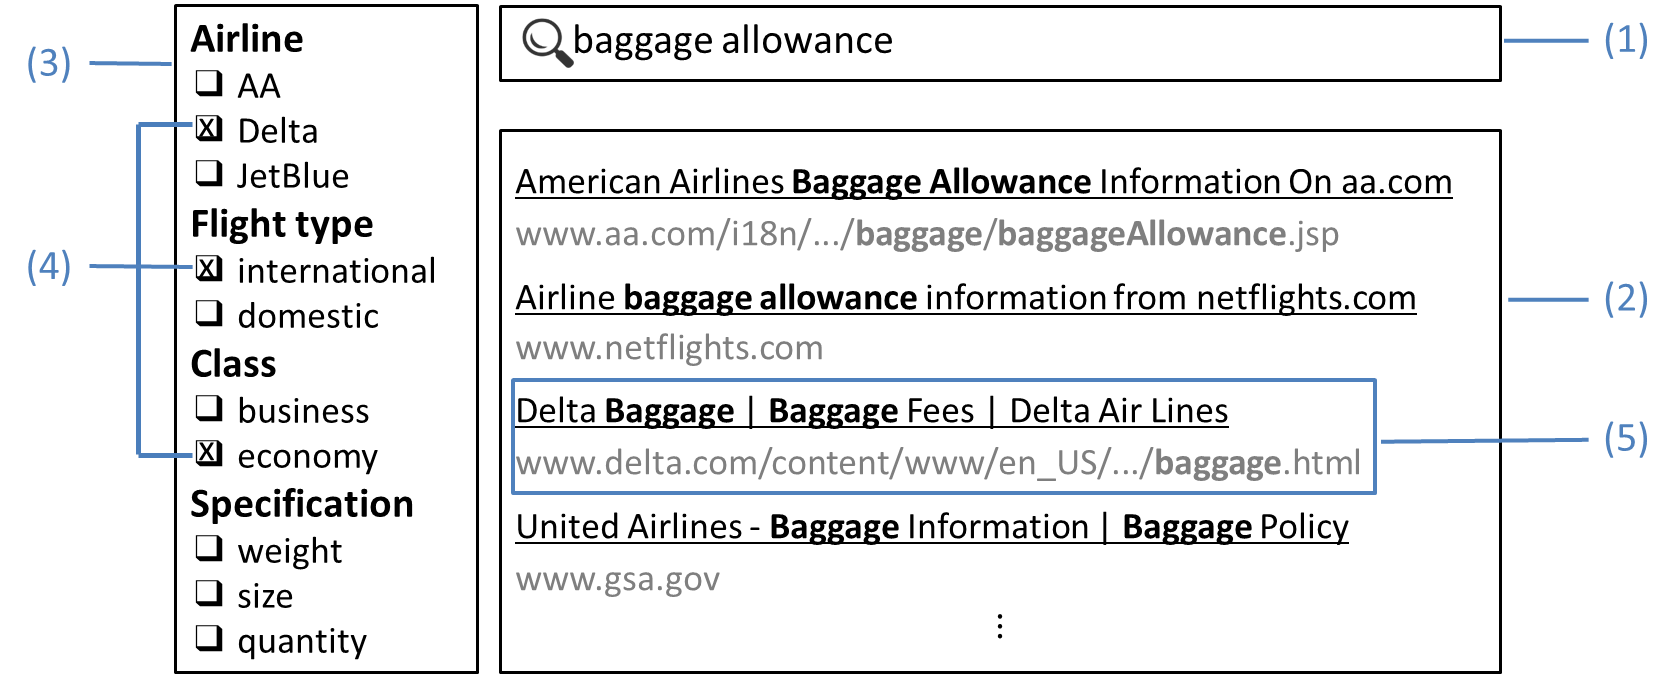
\includegraphics[width=0.97\columnwidth]{figure/fws-example.png}
%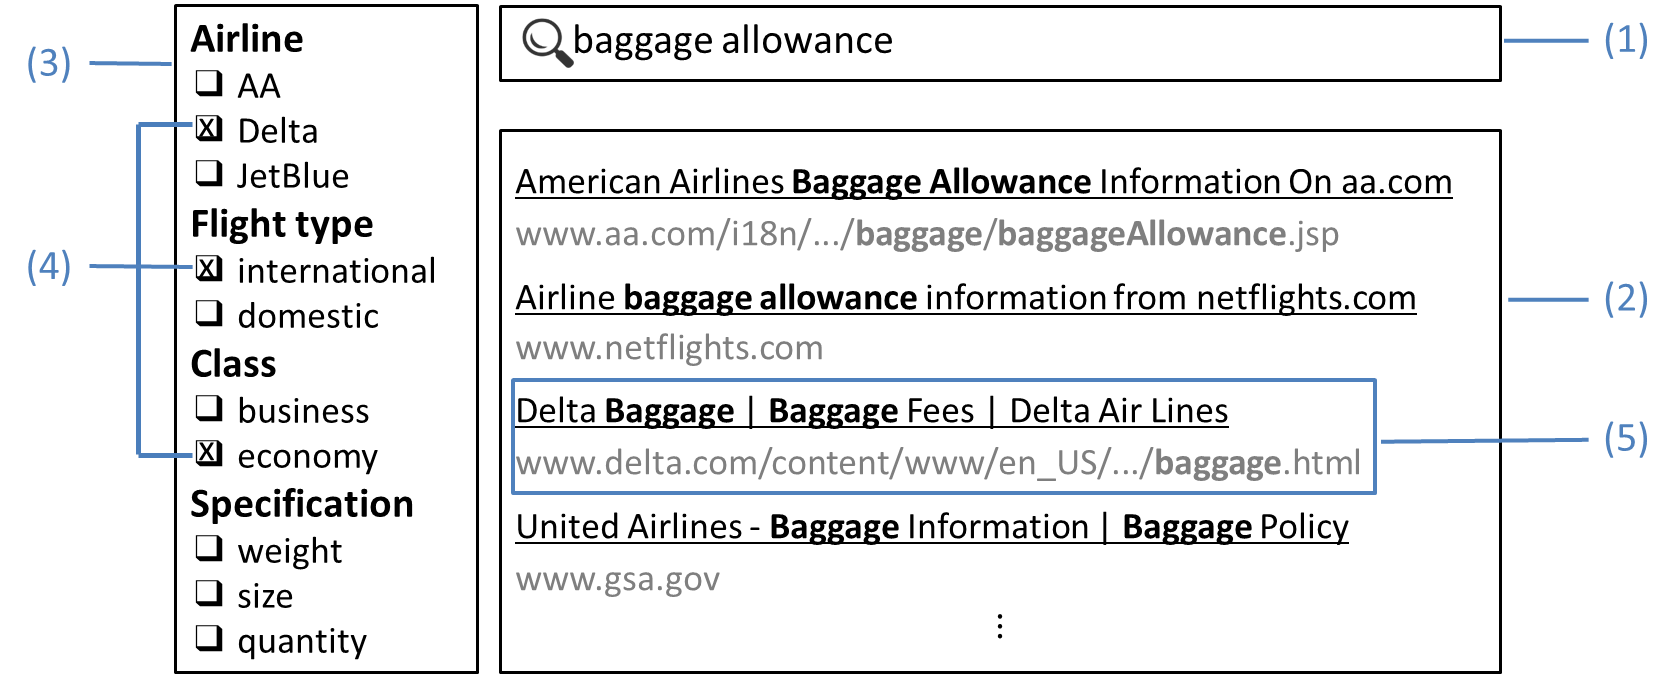
\includegraphics[scale=0.45]{figure/fws-example.png}
\caption{An example of Faceted Web Search: (1) the user issues a query; (2) the system returns search results; (3) the system provides facets for the query; (4) the user selects terms in the facets; (5) the system re-ranks this relevant document to the top according to the selected terms.}
\label{fig:fws-example}
\end{figure}


This thesis address three fundamental issues of Faceted Web Search, including facet generation, facet feedback, and evaluation, as described further as follows.

\subsection{Facet Generation}
Facet generation is to identify facets for navigation (corresponding to step 3 in Figure~\ref{fig:fws-example}). In conventional faceted search, facets are generated in advance for an entire corpus~\cite{stoica2007automating,dakka2008automatic} either manually or semi-automatically, and then recommended for particular queries in most of the previous work~\cite{teevan2008challenges}. However, this approach is difficult to extend to the entire web due to the web's large and heterogeneous nature. We instead propose a query-dependent approach, which extracts facets for a query from its search results, providing a promising direction for solving the problem. 

We call the extracted items ``query facets'', defined as a set of coordinate terms (\eg, \{\concept{AA}, \concept{Delta}, \concept{JetBlue},...\}) that explicitly represent one aspect (\eg, \concept{airlines}) of the query (\eg, \concept{baggage allowance}). The coordinate terms share a semantic relationship by being subsumed by a more general hypernym (\eg, \concept{AA}, \concept{Delt}, \concept{JetBlue} are subsumed by \concept{airlines}). More examples for query facets are shown in Table~\ref{tab:facetexample}. Note that our work dose not generate the hypernym or label (\eg, \concept{airlines}) for the coordinate terms. This definition of query facets corresponds to one-level taxonomies in faceted taxonomy, in which only information objects that belong to a same parent node are shown as a facet (see the definition in Section~\ref{sec:bg-fws}). We leave generating facets as two- or more level taxonomies as future work.

Because it is an automatic task, facet generation in FWS can be imperfect. The system can make mistakes in both precision and recall for generating facets. As in many precision-oriented information retrieval tasks, we believe users are likely to care more about ``facet precision'' than ``facet recall''. That is, users may care more about the correctness of presented facets (\eg, are the terms in the airline facet indeed about airlines, and are the airline terms grouped together in a same facet) than the completeness of facets (\eg, are all possible facets for that query presented, and are all possible airline terms included the results?). In other words, mistakes of presenting wrong terms in a facet, or grouping terms incorrectly are more severe than omitting some facets or terms in facets. Thus, we also study how to improve facet generation performance under precision-oriented scenarios, in order to make the technique more practical.

\subsection{Facet Feedback}
Facet feedback is to use selections on the facets to adjust (\eg, filter or re-rank) the search results (corresponds to step 5 in Figure~\ref{fig:fws-example}). In conventional faceted search, facet feedback is straightforward: as all information objects have been classified in the faceted taxonomy, when users make their selections on the facets, the search results can be easily filtered by requiring each objects belong to the restricted taxonomies according to the selection.

However, in FWS there is no explicit classification of webpages into the generated facets. One solution is Boolean filtering, which filters search results by the requiring selected terms to appear. However, it turns out to be too strict when extended to the open-domain setting. Boolean filtering is based on two assumptions~\cite{zhang2010interactive}: (1) users are clear about what they are looking for, and thus are able to select proper terms to restrict the results; and (2) matching between a term and a document is accurate and complete. In FWS, that means a document that contains the selected term should be relevant to the term, and all documents relevant to that selected term should contain the term. Neither of the two assumptions are likely to hold reliably in FWS. Thus, we also investigate soft ranking models that expand original queries with user selection on the facets.
  

\subsection{Evaluation}
Evaluation for conventional faceted search mostly focuses on its user interface~\cite{burke1996knowledge,english2002hierarchical,hearst2006design,hearst2008uis,kules2009exploratory}. For FWS, there can be two types of evaluation according to the different focuses, namely intrinsic and extrinsic evaluation. Intrinsic evaluation only considers facet generation (i.e., the quality of generated facets).  Extrinsic evaluation instead evaluates the effectiveness of the entire FWS system, combining both the facet generation and facet feedback components. We study both of them.

Most of the previous evaluations for faceted search are based on user studies~\cite{dash2008dynamic,li2010facetedpedia,stoica2007automating}. However, user studies are often very expensive and more importantly difficult to extend for evaluating new systems. We instead design evaluation methods with higher reusability for both intrinsic and extrinsic evaluation.

In the following, we highlight the contributions of this thesis.
\section{Contributions}
\label{sec:intro-contributions}
\begin{itemize}
 \item Faceted Web Search. We define Faceted Web Search, which extends faceted search into an open-domain web setting. We design a framework for an FWS system, which contains the facet generation and facet feedback components. We show that using this faceted search interface can significantly improve the original ranking if allowed sufficient time for user feedback: 18.0\% in NDCG@10 if we allow users to examine 50 terms in facets, and 7.4\% in NDCG@10 if we allow time for examining 10 terms. \todo{interactive}

 \item Query facet extraction. To cope with the large and heterogeneous nature of the web in facet generation, we develop a query-dependent approach, which generates facets for a query instead of the entire corpus. This query facet generation approach extracts facets from the top search results for the issued query. This not only makes the generation problem easier, but also addresses the facet recommendation problem at the same time. For query facet extraction, we develop a supervised approach based on a graphical model to recognize facets from the noisy candidates found. The graphical model learns how likely a candidate term is to be a facet term as well as how likely two terms are to be grouped together in a query facet, and captures the dependencies between the two factors. We propose two algorithms (\QFI and \QFJ) for approximate inference on the graphical model since exact inference is intractable. Compared with other existing methods, our models can easily incorporate a rich set of features, and learn for available labeled data.

\item Intrinsic evaluation. We evaluate the quality of generated facets by comparing them with human-created ones. This can be measured from three aspects -- precision and recall of extracted terms for facets, and the clustering quality of these facet terms. We design \PRF, a measure to combine three evaluation factors together using weighted harmonic mean. This metric has the flexibility to adjust emphasis between the three factors for different applications. We also describe how to collect human annotations for query facets by a pooling method. Experimental results based on this intrinsic evaluation show that our supervised methods (\QFI and \QFJ), can take advantage of a richer set of features and outperform other unsupervised methods, such as pLSA, LDA, and a variant of quality threshold clustering model~\cite{dou2011finding}. \todo{pooling for annotation}

\item Precision-oriented query facet extraction. We improve query facet extraction performance under precision-oriented scenarios from two perspectives. First, we find that the likelihood objective used in the query facet extraction model can be loosely related to the performance measure in the precision-oriented scenario. Therefore, we directly optimize the performance measure instead of likelihood during training using a empirical utility maximization approach. However, exact optimization on the performance measure is difficult due to the non-continuous and non-differentiable nature of information retrieval measures. We address this problem by approximating the performance measure using its expectation. We show that this empirical utility maximization approach significantly improves models under precision-oriented scenarios, suggesting that utility is a better learning objective than likelihood, and that our expectation-based approximation is effective.  


\item Second, we improve extraction performance by a selective method that shows facets for good performing queries and avoids doing so for poor performing ones. We find that extraction performance varies for different queries -- some queries are naturally more difficult than others for extracting query facets. In the precision-oriented scenario, it may be more desirable to avoid showing facets for those poor performing queries and leave the users with a clean keyword-search interface. A key problem, however, is how to predict the extraction performance. To solve this problem, we develop a simple and effective score based on the expectation of the performance measure. We find the score has a strong correlation with the performance measure, and when used in the selective method, it can significantly improve the average performance with fair coverage over the whole query set.

 
\item Facet feedback. We find that Boolean filtering models are too strict for FWS, and propose soft ranking models that expand original queries with user selected terms in facets for re-ranking. We show that the proposed soft ranking models are more effective than Boolean filtering models, which are widely used in conventional faceted search.
 
\item Extrinsic evaluation. We develop an extrinsic evaluation method that evaluates FWS systems by their utility in assisting search clarification. This evaluation considers both gain in ranking improvement and cost in time for users to give feedback. Instead of performing user studies, we simulate the user feedback process, so that we can easily extend the evaluation for new models or systems. The simulation is based on a simple user model of the feedback process and limited human annotations.

\item Building a reusable test collection. We describe a way of building reusable test collections for the intrinsic and extrinsic evaluation. We make our collected data set publicly available. The data set consists of annotated facets for 196 TREC Web Track queries from 2009 to 2012, and simulated user feedback for 678 corresponding query subtopics.

%\item A demonstration system for Faceted Web Search. We develop a demonstration system
%%\footnote{It is currently online in http://brooloo.cs.umass.edu/}
%for Faceted Web Search. The demonstration system shows extracted query facets for a given query online. The system now supports querying over the entire web using Bing Search API\footnote{https://datamarket.azure.com/dataset/bing/search}, and ClueWeb09 corpus\footnote{http://lemurproject.org/clueweb09} based on Galago Search Engine\footnote{http://www.lemurproject.org/galago.php}.
\end{itemize}

\section{Outline}
The remainder of this thesis is organized as follows. 
In Chapter~\ref{ch:bg}, we provide background information related to this thesis. In Chapter~\ref{ch:facet}, we present our query facet extraction approach. 
In Chapter~\ref{ch:intrinsiceval}, we present our intrinsic evaluation that evaluates generated facets by comparing them with human-created ones.
In Chapter~\ref{ch:precision}, we investigate query facet extraction models under precision-oriented scenarios, and improve our models in such scenarios.
In Chapter~\ref{ch:feedback}, we investigate both Boolean filtering and soft ranking models for facet feedback.
In Chapter~\ref{ch:extrinsiceval}, we develop our extrinsic evaluation method that evaluates entire Faceted Web Search systems in terms of their utility in assisting search in an interactive search task.
Lastly, in Chapter~\ref{ch:conclusions}, we summarize the contributions made in this thesis and discuss potential future directions for more research in this area.





\chapter{Background}
\label{ch:bg}
In this chapter, we discuss background information and related work for Facet Web Search, an extension of faceted search in the open-domain web setting. Faceted search is a heavily interdisciplinary area, where different aspects of information retrieval, knowledge representation, human computer interaction must be considered all together. Therefore, we first describe related topics in these areas as a background for faceted search/Faceted Web Search. Then, we describe faceted search, Faceted Web Search and previous research on these topics. After that, we discuss related approaches that aim to achieve the same goals as Faced Web Search. We defer discussion of some related work to later chapters where the context makes it more appropriate.

\section{Direct Search and Navigational Search}
Faceted search combines two search paradigms, direct search and navigational search. \textbf{Navigational search} (sometimes also called \concept{directory navigation}) uses a hierarchy structure to enable users to browse the information space by iteratively narrowing the scope of their quest in a predetermined order, as exemplified by Yahoo! Directory\footnote{http://en.wikipedia.org/wiki/Yahoo!\_Directory} and DMOZ\footnote{http://www.dmoz.org/}. Navigational search provides a guided search interface, and supports abstractions that are easily understood by users. However, the strict ordering imposed by the hierarchy structure can be too rigid, especially for large and heterogeneous corpora~\cite{snow2006semantic,tunkelang2009faceted,sacco2009dynamic}. The rapid decline of Yahoo! Directory as a primary web search engine provides pragmatic evidence.

\textbf{Direct search} instead allows users to specify their own queries as input, and is the dominant paradigm in the field of information retrieval. The queries are often keywords in web search scenarios, and thus, sometimes direct search is also called \concept{keyword search}. Direct search resorts to search systems for understanding search intents behind user queries, and returns search results that could best address the search intents. This approach has been made enormously popular by web search engines, such as Google\footnote{http://www.google.com}. However, in the basic search interface, users have to formulate their queries with no or limited assistance, and no exploration capability since results are presented as a flat list with no systematic organization. Faceted search aims to solve this problem, which is described later in Section~\ref{sec:background-fs}. We also discuss other recent advances for addressing this problem in Section~\ref{sec:bg-others}.

\section{Taxonomy and Faceted Taxonomy}
There are two types of information representation (or knowledge representation) related to this work, taxonomies and faceted taxonomies. A \textbf{taxonomy} is an organization of information objects or abstractions into a hierarchy or tree structure~\cite{tunkelang2009faceted}. Navigational search as described above is based on taxonomies. So we have seen two examples of taxonomies, Yahoo! Directory and the Open Directory Project, in which webpages are classified into the hierarchies. An older example is Aristotle's system for organizing knowledge of the human race~\cite{tunkelang2009faceted}. The system classifies living things by dividing them into two groups, plants and animals; further dividing animals into those ``with blood'' and ``without blood''; those with blood into ``live-bearing'' and ``egg-bearing''; and so forth (Figure~\ref{fig:bg-aristotle}).

\begin{figure}[ht!]
\centering
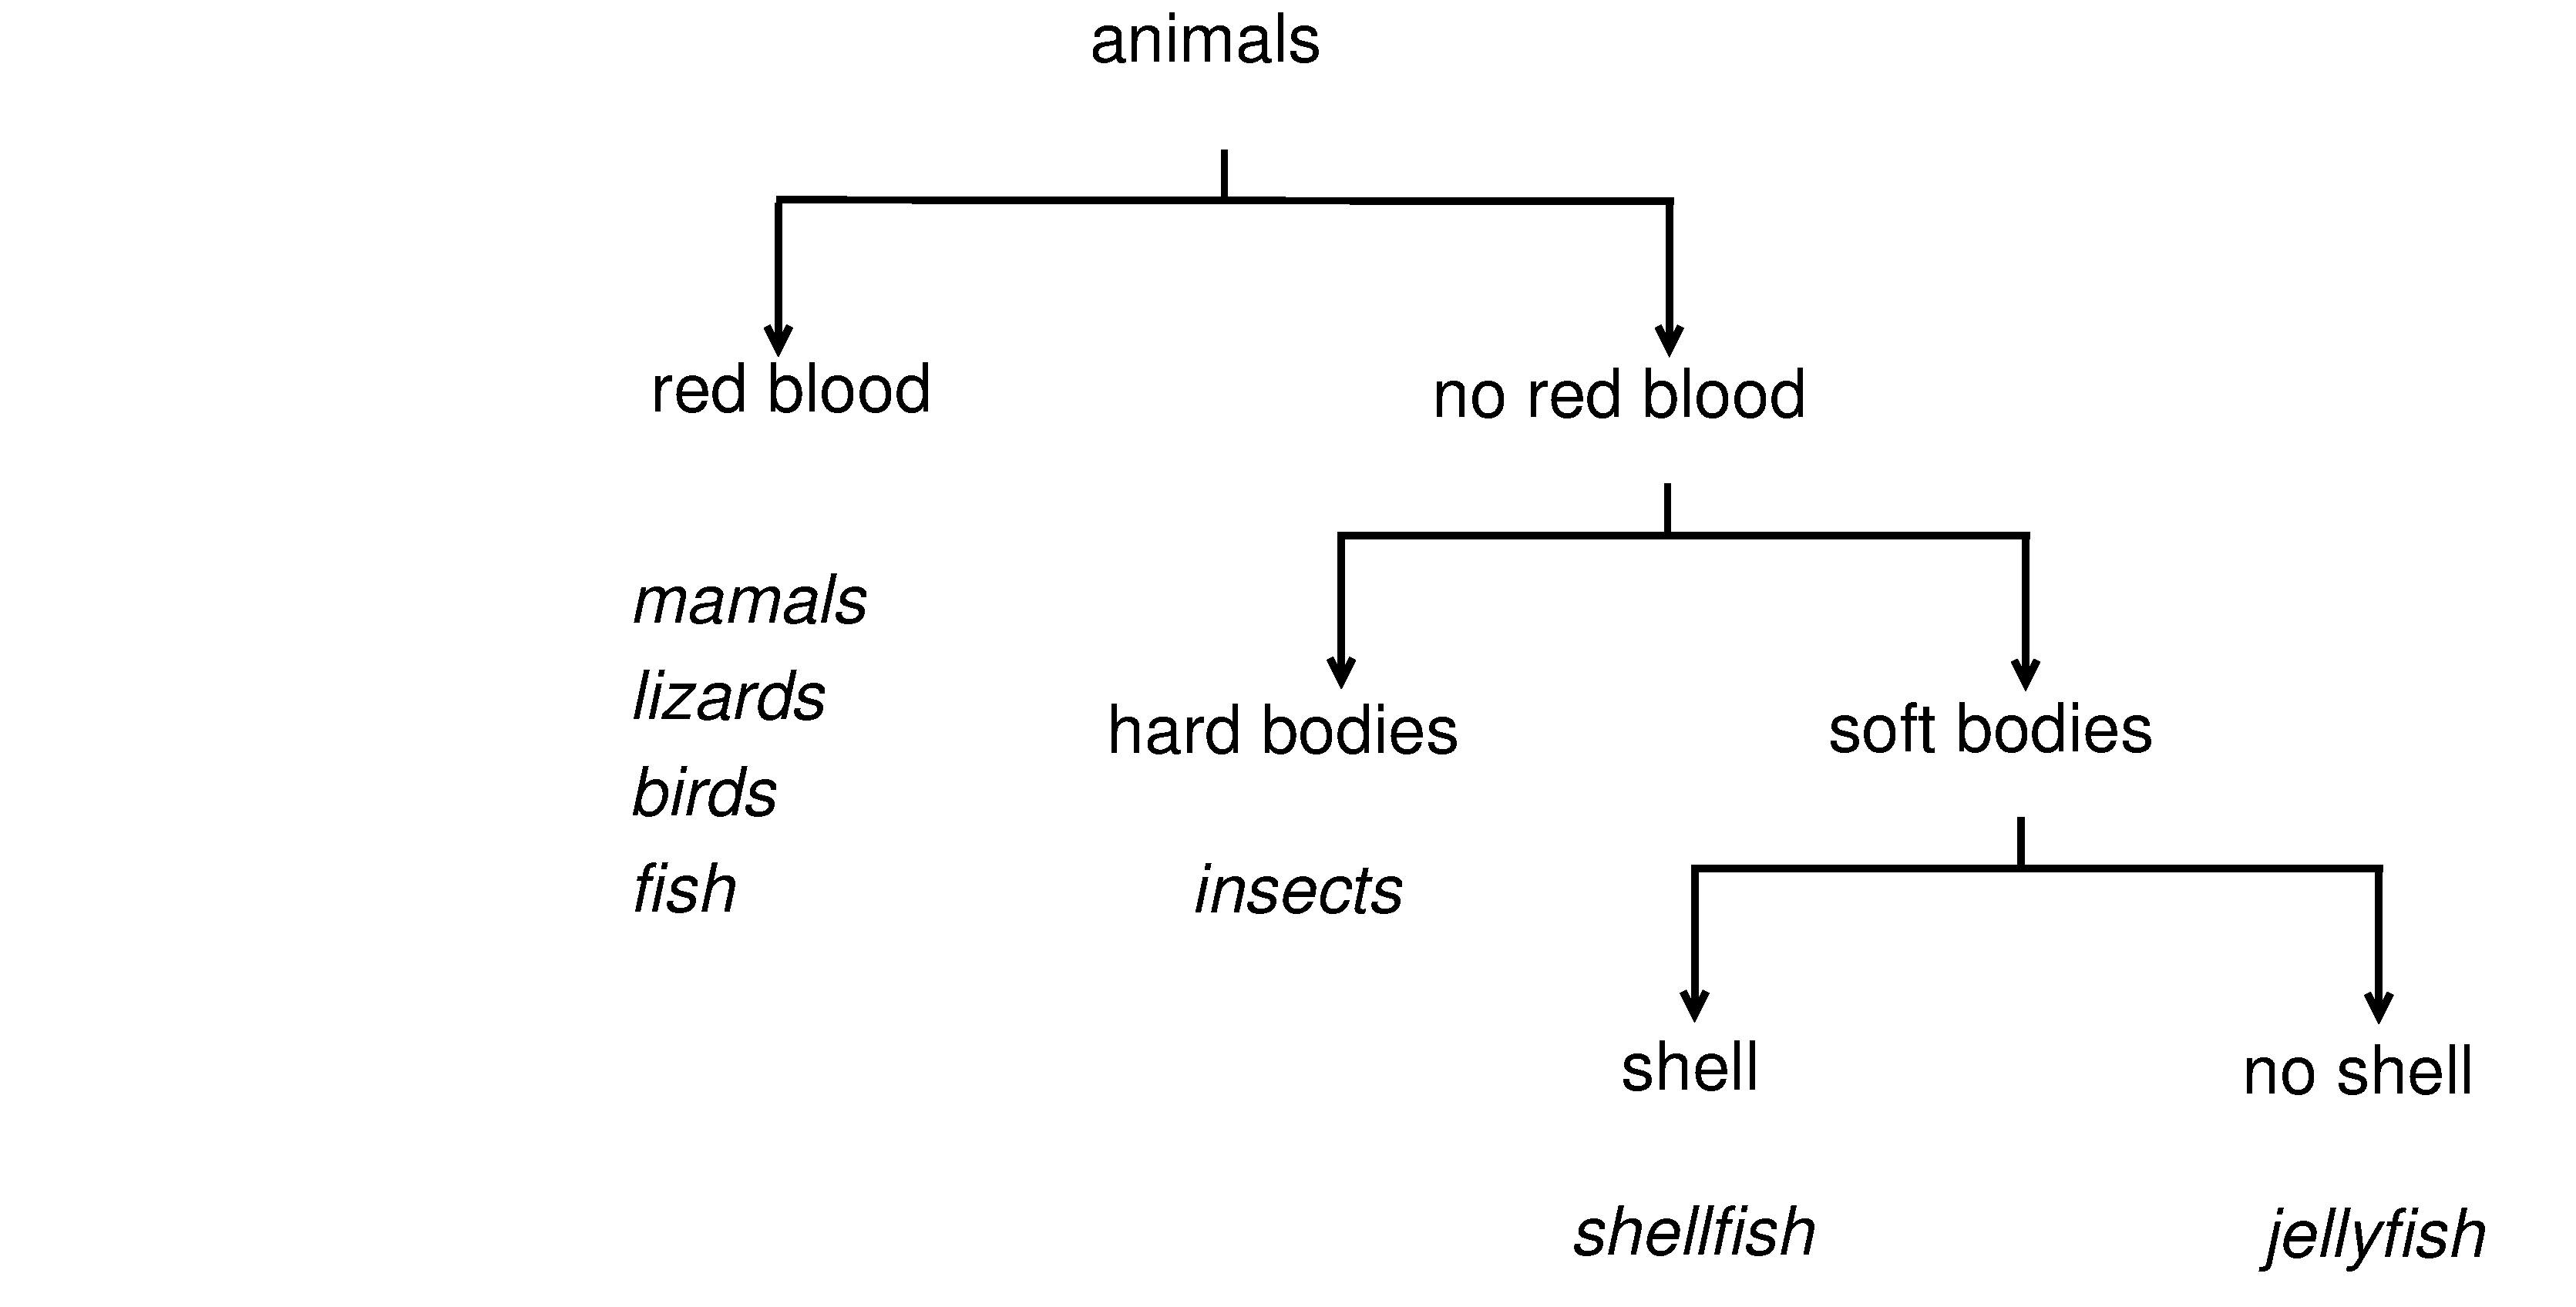
\includegraphics[width=0.95\columnwidth]{drawing/aristotle.eps}
\caption{A subset of Aristotle's knowledge taxonomy~\cite{tunkelang2009faceted}}
\label{fig:bg-aristotle}
\end{figure}

In the context of navigational search, taxonomy enables efficient navigation in the information space. Users start from the root node and iteratively discriminate among children, in order to find the appropriate one. Each time a node is selected for expansion, the total number of objects to be considered is reduced because the objects classified under discarded concepts need not be considered. Thus, users iteratively reduce the number of information objects to be manually inspected~\cite{sacco2009dynamic}.

The key property of a taxonomy is that, for every information object or set of objects that corresponds to a node, there is precisely one unique path to it from the root node. Thus, a taxonomy imposes a strict logical ordering on the information that it represents~\cite{tunkelang2009faceted}. For example, \concept{cancer} can be classified in a taxonomy with a unique path  \concept{disease}$\rightarrow$\concept{structural disease}$\rightarrow$\concept{tumor}$\rightarrow$\concept{cancer}. However, this strict ordering of a taxonomy can be too rigid when dealing with compound information objects. For example, should \concept{treatment of cancer} be a child of \concept{treatment} or of \concept{cancer}? This strict ordering constraint limits expressibility and extensibility of taxonomies and navigational search systems build on them.

Faceted search is based on another type of information representation, called faceted taxonomy, which is sometimes also called multi-dimensional  taxonomy~\cite{sacco2009dynamic} or faceted classification~\cite{tunkelang2009faceted}. A \textbf{faceted taxonomy} is a set of independent taxonomies where each one organizes information objects from a different (preferably orthogonal) point of view, or equivalently based on a different dimension of the multi-dimensional information space. For example, in \textit{Classification, Coding, and Machinery for Search}, \citet{ranganathan1950classification} describe a library system based on a faceted taxonomy for organizing books, with four independent taxonomies mentioned -- the taxonomy \concept{Medicine}, \concept{Disease}, \concept{Treatment} and \concept{Mathematical study}. The four taxonomies each represents one dimension of the multi-dimensional information space for the books. \todo{better example for faceted taxonomy}


The advantage of using multiple independent taxonomies is that they can be combined to describe compound information objects. In Ranganathan's example, the four taxonomies are combined to expresses the topic \concept{statistical study of the treatment of cancer of the soft palate by radium}, as follows. 
\begin{itemize}
 \item Medicine $\rightarrow$ Digestive system $\rightarrow$ Mouth $\rightarrow$ Palate $\rightarrow$ Soft palate
\item Disease $\rightarrow$ Structural disease $\rightarrow$ Tumor $\rightarrow$ Cancer
\item Treatment $\rightarrow$ Treatment by chemical substances $\rightarrow$ Treatment by a chemical element  $\rightarrow$ Treatment by a group 2 chemical element $\rightarrow$ Treatment by radium
\item Mathematical study $\rightarrow$ Algebraical study $\rightarrow$ Statistical study
\end{itemize}
The foci (\concept{Soft palate}, \concept{Cancer}, \concept{Treatment by radium} and \concept{Statistical study}) in each of the taxonomies are combined to express the compound topic, which is difficult in a single hierarchical taxonomy. Combining these independent taxonomies, faceted taxonomies offer expressive power and flexibility beyond single taxonomy used in navigational search. 

%From the example, we can also see that faceted taxonomy enables navigation over , which is called \textbf{faceted navigation}.
Navigation based on a faceted taxonomy is called \textbf{faceted navigation}. In faceted navigation, users can use multiple taxonomies to navigate or explore a multi-dimensional information space. They can narrow the search space by iteratively select child nodes in each of taxonomies. Then the selections on the taxonomy are combined to restrict the matched information objects, as has illustrated in Ranganathan's example. 
\todo{add an example}
\todo{relationships to scatter/gather, clustering}

%pose a challenge for the hierarchical organization of single taxonomies.
\section{Facets}
``Facet'' is a key concept in faceted search. The term \concept{facet} means ``little face'' and is often used to describe one side of a many-sided object, especially a cut gemstone~\cite{teevan2008challenges}. In information science literature, \concept{facet} is a overloaded term. The term has been used to refer both to the entire independent taxonomies in a faceted taxonomy, and to the part of independent taxonomies that are shown to users (as in most of our discussion). In many cases the taxonomies are often shown as shallow or two-level trees. In the computer monitor example (Figure~\ref{fig:intro-amazon}), the facets are two-level (\eg, parent node \concept{Brand} with child nodes \concept{Dell}, \concept{ViewSonic}, \concept{HP}, \concept{Acer}). When there are only two levels in a facet, we can call the parent node (or more precisely, its presentation term) a \textbf{facet label} (\eg, \concept{brand}), and the child nodes \textbf{facet terms} (\eg, \concept{Dell}, \concept{ViewSonic}). It is easy to see that in a two-level facet, facet terms belong to the same semantic class (\ie, the semantic class represented by their parent node). Sometimes, a facet label can be missing or omitted, which results in a one-level facet. So a one-level facet consists of only the facet terms (\eg, \{\concept{Dell}, \concept{ViewSonic}, \concept{HP}, ...\}) with no facet label. This work focuses on studying one-level facets for Faceted Web Search as a start, and leaves the extension of two-level facets to future work.

\todo{exploratory search}

\section{Faceted Search}
\label{sec:background-fs}
\textbf{Faceted Search} combines direct search with faceted navigation, which enables users to navigate a multi-dimensional information space. We have provided an example in Figure~\ref{fig:intro-amazon}. In the example, a user searches with the query \concept{computer monitor} in an e-commercial site, and the site provides the two-level facet \concept{brand}, \concept{display technology} and \concept{condition} for users to select and filter the search results.

Compared with direct search, faceted search provides additional search assistance for users through facets. Facets can assist users in clarifying their search intent and refining the search results (\eg, select \concept{new} in facet \concept{condition} to find only computer monitors in new conditions). Facets also summarize the search space succinctly, and provides exploration suggestions organized in a systematic way (\eg, the listed facet \concept{brand}, \concept{display technology}, \concept{condition} give users an overview of the returned results, and provides them with the key factors they may need to consider when searching for a computer monitor). This exploration capability is especially important in exploratory search tasks, or when users are not exactly clear about what they are looking for~\cite{kules2009exploratory,sacco2009dynamic}.

Compared with navigational search, faceted search supports faceted navigation, which, as outlined above, is especially useful for navigating a multi-faceted information space. In navigational search, the strict ordering imposed by a taxonomy is too rigid when dealing with compound information objects in the multi-faceted information space. Instead, in faceted search, users can combine facets to express complex information need (\eg, \concept{statistical study of the treatment of cancer of the soft palate by radium} in  Ranganathan's example).

\subsection{Automatic Facet Generation}
Previous work on faceted search has studied automatic facet generation ~\cite{dakka2008automatic,li2010facetedpedia,stoica2007automating,oren2006extending,kohlschutter2006using,latha2010afgf} and facet recommendation for a query~\cite{dash2008dynamic,koren2008personalized}. Most of the work is based on existing facet metadata or taxonomies, and extending faceted search to the general web is still an unsolved problem. The challenges stem from the large and heterogeneous nature of the web~\cite{teevan2008challenges}: because the web is very large, it is
difficult to assign quality facets to every document in the collection and to retrieve the full set of search results and their associated facets at query time; and because the web is heterogeneous, it is difficult to apply the same facets to every search result or every query.
%Different from previous work which generates facets for a entire corpus~\cite{stoica2007automating,dakka2008automatic}, some recent work~\cite{dou2011finding,kong2013extracting} extracts facets for only a query.

\subsection{Evaluation for Faceted Search}
Most evaluations for facet generation/recommendation are either based on comparison between system generated and human created facets~\cite{dakka2008automatic,dou2011finding} or user studies~\cite{dash2008dynamic,li2010facetedpedia,stoica2007automating}. However, the former may not exactly reflect the utility of assisting users' search tasks, and the latter is expensive to extend for evaluating new systems. In a spirit similar to ours, some work~\cite{schuth2011evaluation,zhang2010interactive,koren2008personalized} also evaluates facets by their utility in re-ranking documents for users. The differences are their evaluation methods do not capture the time cost for users as explicitly as we do, and their experiments are based on corpora with human created facet metadata. Other evaluations~\cite{burke1996knowledge,english2002hierarchical,hearst2006design,hearst2008uis,kules2009exploratory} for faceted search are mostly done from a user interface perspective, which is beyond the scope of 
this proposal.

\section{Other Related Techniques}
\label{sec:bg-others}
A number of other areas are similar in spirit to ours, We discuss query subtopic mining, semantic class extraction, search result diversification and search result clustering/organization.
\subsection{Query Subtopic/Aspect Mining}
To address multi-faceted queries, much previous work studied mining query subtopics (or aspects). 
A query subtopic is often defined as a distinct information need relevant to the original query.
It can be represented as a set of terms that together describe the distinct information need~\cite{wang2009mining,wu2011identifying, dang2011inferring} or as a single keyword that succinctly describes the topic~\cite{song2011overview}. 
Different resources have been used for mining query subtopics, including query logs~\cite{wang2007learn,hu2012mining,xue2011topic,wang2009mining,wu2011identifying,yin2010building}, document corpus~\cite{allan2002using} and anchor texts~\cite{dang2011inferring}.
\todo{top-ranked docs?}
% Much work~\cite{Wang:2007:LWS:1277741.1277759, Hu:2012:MQS:2348283.2348327} uses related queries from search logs as candidates, and clustered them into query subtopics. Wang and Zhai~\cite{Wang:2007:LWS:1277741.1277759}, for example, used snippets of a query's clicked web documents to enrich the query representation, and then cluster related past queries into query subtopics.
%Due to data sparsity for instance-level query subtopics, Some work~\cite{Wang:2009:MBL:1557019.1557114,Xue:2011:TMN:2063576.2063877,Wu:2011:IAW:2016945.2016963,Yin:2010:BTW:1772690.1772792} mined generic query subtopics, which are query subtopics for a generic class of queries.
%For example, Yin et al.~\cite{Yin:2010:BTW:1772690.1772792} built taxonomies of query subtopics for categories of name entity queries using search logs.
%Wu et al.~\cite{Wu:2011:IAW:2016945.2016963} also worked on identifying query aspects for named entities queries. They propagated reformulation phrases for a classes of named entities queries.
%Other than query logs, query subtopics can also be mined from documents. For example, Dang et al.~\cite{Dang:2011:IQA:2063576.2063904} worked on clustering related anchor texts in ClueWeb09 corpus into query subtopics. Allan et al.~\cite{Allan:2002:UPP:564376.564430}, from a text corpus, extracted commonly occurring parts of speech pattern near a single-word query to find different potential specifications of the query.


Query subtopics and facets for a query are different in that the terms in a query subtopic are not restricted to be coordinate terms, or to have peer relationships. Facets for a query, however, organize terms by grouping ``sibling'' terms together. For example, \{\textit{news}, \textit{cnn}, \textit{latest news}, \textit{mars curiosity news}\} is a valid query subtopic for the query \textit{mars landing}, which describes the search intent of Mars landing news, but it is not a valid facet. Instead, a valid facet that describes Mars landing news could be \{\textit{cnn}, \textit{abc}, \textit{fox}\}, which includes different news channels.
%In a recent work~\cite{Dou:2011:FDQ:2063576.2063767}, Dou et al. developed a system to extract facets from web search results and showed the potential of doing so. However, the unsupervised method they proposed is far from optimal, and it does not improve by having human labels available. Also, to the best of our knowledge, their evaluation can be problematic in some cases, which will be discussed in Section~\ref{sec:evalmetricsall}.

\subsection{Semantic Class Extraction}
Semantic class extraction is to automatically mine semantic classes represented as their class instances from certain data corpora. For example, it may extract \textit{USA}, \textit{UK}, \textit{China} as class instances of semantic class \textit{country}. Due to the similar semantic relationships between terms inside a facet and a semantic class, semantic class extraction can be used for facet generation. Existing approaches can be roughly divided into two categories: distributional similarity and pattern-based~\cite{shi2010corpus}. The distributional similarity approach is based on the distributional hypothesis~\cite{Harris}, that terms occurring in analogous contexts tend to be similar. Different types of contexts have been studied for this problem, including syntactic context~\cite{pantel2002discovering} and lexical context~\cite{pantel2004towards,agirre2009study,pantel2009web}.
The pattern-based approach applies textual patterns~\cite{hearst1992automatic,pasca2004acquisition}, HTML patterns~\cite{shinzato2007simple} or both~\cite{zhang2009employing,shi2010corpus} to extract instances of a semantic class from some corpus.
The raw semantic class extracted can be noisy. To address this problem, \citet{zhang2009employing} used topic modeling to refine the extracted semantic classes.
Their assumption is that, like documents in the conventional setting, raw semantic classes are generated by a mixture of hidden semantic classes.\todo{describe similarity}
In this work, we apply pattern-based semantic class extraction on the top-ranked Web documents to extract candidates for query facet generation.

\subsection{Search Results Diversification}
Search result diversification has been studied as a method of tackling ambiguous or multi-faceted queries while a ranked list of documents remains the primary output feature of Web search engine today~\cite{agrawal2009diversifying,clarke2008novelty,santos2010exploiting,sakai2011evaluating,dang2013term}.
The purpose is to diversify the ranked list to account for different search intents or query subtopics.
A weakness of search result diversification is that the query subtopics are hidden from the user, leaving him or her to guess at how the results are organized.
FWS addresses this problem by explicitly presenting different facets of a query using groups of coordinate terms for users to select.
\todo{difference}

\subsection{Search Result Clustering/Organization}
Search results clustering is a technique that tries to organize search results by grouping them into, usually labeled, clusters by query subtopics~\cite{carpineto2009survey}.\todo{change citation}
It offers a complementary view to the flat ranked list of search results.
Most previous work has exploited different textual features extracted from the input texts and applied different clustering algorithms with them.

Instead of organizing search results in groups, there is also some work~\cite{lawrie2001finding,lawrie2003generating, nevill1999lexically} that summarizes search results or a collection of documents in a topic hierarchy. For example, previous studies~\cite{lawrie2001finding,lawrie2003generating} used a probabilistic model for creating topical hierarchies, in which a graph is constructed based on conditional probabilities of words, and the topic words are found by approximately maximizing the predictive power and coverage of the vocabulary. \todo{similar to taxonomy}

FWS is different from these work in that it provides facets of a query, instead of directly organizing the search results. The facet interface allows users to filter/re-rank search results from multiple aspects, instead of a single, taxonomic order.

%\section{User Feedback}
%There is a long history of using user explicit feedback to improve retrieval performance. In relevance feedback~\cite{rocchio71relevance,salton90improvingretrieval}, documents are presented to users for judgment, after which terms are extracted from the judged relevant document, and added into the retrieval model. In the case where true relevance judgments are unavailable, top documents are assumed to be relevant, which is called pseudo relevance feedback~\cite{buckley1995automatic,abdul2004umass}. Because a document is a large text unit which can be difficult for users to judge and for the system to incorporate relevance information, previous work also studied user feedback on passages~\cite{allan1995relevance,xu1996query} and terms~\cite{koenemann1996case,tan2007term}.

%For faceted search, previous work~\cite{zhang2010interactive} studied user feedback on facets, using both boolean filtering and soft ranking models. However, the study is based on corpora with human created facet metadata, which is difficult to obtain for the general web. One other difference between our work and most other user feedback work is, facet feedback in our work is used to improve ranking with respect to the query subtopic specified by the feedback terms, instead of the query topic represented by the original query. This presents the scenario in FWS, where users start with a less-specified query, and then use facets to help clarify and search for subtopic information.

\section{Summary}
\todo{re-state facet and facet term definition here}
Faceted web search (FWS) we propose in this work is different from all the past work. It extends conventional faceted search from a fixed-domain setting to an open-domain web setting. It is different from search result diversification in that instead of hiding those query subtopics from users, it explicitly presents different facets of a query. It is also different from search results clustering or organization in that instead of directly organizing the search results, the facet interface in FWS allows users to filter/re-rank search results from multiple aspects.

We study three main issues of FWS that have not been explored in previous work, including facet generation, facet feedback and evaluation for FWS. Facet generation for FWS is different from query subtopic mining due to the different nature of query subtopics and facets. It is also different from semantic class extraction in that it targets a general web query instead of a semantic class. Facet feedback for FWS is different from other user feedback due to their different purposes. Facet feedback targets at improving ranking with respect to the ``query subtopic'' specified by the feedback terms, instead of the query topic represented by the original query. Our evaluation for FWS is also different from previous ones for faceted search. We consider many different aspects (e.g., cost and gain), and the evaluation is based on simulations instead of user studies, which makes it relative cheap to extend for new systems. \todo{the evaluation description is not in this chapter}

\chapter{Query Facet Extraction}
\label{ch:facet}
\section{Introduction}
In conventional faceted search, facets are typically generated in advance for an entire corpus~\cite{stoica2007automating,dakka2008automatic} either manually or semi-automatically, and then recommended for particular queries. However, this approach is difficult to extend to faceted web search due to the large and heterogeneous nature of the web~\cite{teevan2008challenges}: because the web is very large, it is
difficult to assign quality facets to every document in the collection and to retrieve the full set of search results and their associated facets at query time; and because the web is heterogeneous, it is difficult to apply the same facets to every search result or every query.

To cope with this challenge, in this chapter, we propose an alternative solution, called \textbf{query facet extraction}, which extracts facets for queries from their web search results. For example, when users search with the query \concept{baggage allowance}, the system might extract query facets like airlines, \{\concept{Delta}, \concept{JetBlue}, \concept{AA}, ...\}, travel classes, \{\concept{first}, \concept{business}, \concept{economy}\}, and flight types, \{\concept{international}, \concept{domestic}\}. Changing from a global approach that generates facets in advance for an entire corpus to a query-based approach that extract facets from the top-ranked search results, query facet extraction appears to be a promising direction for solving the open-domain faceted search problem -- it not only make the facet generation problem easier, but also addresses the facet recommendation problem at the same time.


We define a \textbf{query facet} as a set of coordinate terms (\eg, \{\concept{AA}, \concept{Delta}, \concept{JetBlue},...\}) that explicitly represent one aspect (\eg, \concept{airlines}) of its query (\eg, \concept{baggage allowance}). The coordinate terms share a semantic relationship by being grouped under a more general hypernym (``is a'' relationship, \eg, \concept{AA}, \concept{Delt}, \concept{JetBlue} are all \concept{airlines}). 
% Terms in query facet are generally called \textbf{facet terms}. When it is clear from context, we will simply use ``facet'' for ``query facet'', and ``term'' for ``facet term'' for convenience. Based on these definitions, \textbf{query facet extraction} is to extract query facets for a given query from certain resources, and in our case the top search results for that query.
In Table~\ref{tab:facet-facetexample}, we show query facets for three example queries. We will using the first query \concept{Mars landing} as example for explanation. For the first query, the first query facet, \{\textit{Curiosity}, \textit{Opportunity}, \textit{Spirit}\}, includes different Mars rovers. The second query facet, \{\textit{USA}, \textit{UK}, \textit{Soviet Union}\}, includes countries relevant to Mars landings. These are both facets where the terms are instances of the same semantic class. 
Somewhat differently, the last facet, \{\textit{video}, \textit{pictures}, \textit{news}\}, includes labels for different query subtopics. These labels can be viewed as instances of a special semantic class, the subtopics of the query \textit{mars landing}. 
\begin{table}[ht!]
\centering
\caption{Query facet examples for three queries}
\label{tab:facet-facetexample}
\begin{tabular}{|l|} \hline
Query 1: Mars landing \\\hline
Query Facet 1: Curiosity, Opportunity, Spirit \\
Query Facet 2: USA, UK, Soviet Union \\
Query Facet 3: video, pictures, news \\\hhline{|=|}
Query 2: baggage allowance \\\hline
Query Facet 1: AA, Delta, Jetblue,  ... \\
Query Facet 2: international, domestic \\
Query Facet 3: first class, business class, economy class \\
Query Facet 4: weight, size, quantity \\\hhline{|=|}
Query 3: Mr Bean \\\hline
Query Facet 1: comics, movies, tv, books \\
Query Facet 2: The Curse of Mr Bean, Mr Bean Goes to Town, ...\\
Query Facet 3: Rowan Atkinson, Richard Wilson, Jean Rochefort,  ...\\ 
Query Facet 4: Mr Bean, Irma gobb, Rupert, Hubert, ...\\\hline
\end{tabular}
\end{table}


In this work, we use query facet extraction to address the problem of facet generation in Faceted Web Search. This approach first extracts candidate facets from the top search results based on textual and HTML patterns, and then refines the extracted candidates, which are often very noisy, using clustering methods. We develop a supervised method based on a graphical model for refining facet candidates. The graphical model learns how likely it is that a term should be selected from the candidates and how likely it is that two terms should be grouped together in a query facet. Further, the model captures the dependencies between the two factors. We propose two algorithms for approximate inference on the graphical model since  exact inference is intractable. This proposed method can easily incorporate a rich set of features and learn from available human labels.
%Also, we design an evaluation metric for query facet extraction, which combines recall and precision of the facet term, with the grouping quality.
%The evaluation metrics will be discussed in Chapter~\ref{ch:intrinsiceval}.

The rest of this chapter is organized as follows. We first define the task of query facet extraction and related concepts in Section~\ref{sec:facet-task}, and then describe a general framework to solve this problem in Section~\ref{sec:facet-framework}. We propose a supervised clustering method based on a graphical model for refining extracted candidates in Section~\ref{sec:facet-gm}. Last, we describe other methods that can be used for refining extracted candidates, including topic modeling (e.g., pLSA, LDA) and a variation of quality threshold clustering model~\cite{dou2011finding} in Section~\ref{sec:facet-other}. 
%The work in this chapter is completed and published~\cite{kong2013extracting}.

\section{Task Description}
\label{sec:facet-task}
\subsection{Query Facet}
To differentiate our work with facets in conventional faceted search, we call typically facets for a particular query ``query facets''. A query facet is a set of coordinate terms -- i.e., terms that share a semantic relationship by being grouped under a more general hypernym (``is a'' relationship), and they succinctly represent different options in the same category that a user can select to refine the issued query. This definition of query facets corresponds to one-level taxonomies in faceted taxonomy, in which only information objects that belong to a same parent node are shown as a query facet. We leave generating query facets as two or more level taxonomies in future work.

\subsection{Facet Term}
We call the terms inside facets ``facet terms'', which can be single words (e.g. \concept{international}, \concept{domestic} in Table~\ref{tab:facet-facetexample}) or phrases (e.g. \concept{first class}, \concept{business class} in Table~\ref{tab:facet-facetexample}). 
These facet terms can be instances of a semantic class, for example \concept{Curiosity}, \concept{Opportunity}, \concept{Spirit} are all Mars rovers. They can be labels for query subtopics, such as \concept{video}, \concept{pictures}, \concept{news} for the query \concept{mars landing}. Facet terms of a query succinctly represent different options in the same category that a user can select to refine the issued query. 

When it is clear from context, we will simply use ``facet'' for ``query facet'', and ``term'' for ``facet term'' for convenience.

\subsection{Query Facet Extraction}
Based on the definitions above, query facet extraction is to extract query facets for a given query from certain resources. While a variety of different resources can be used for query facet extraction, such as a query log, anchor text, taxonomy and social folksonomy, In this work, we only focus on extracting query facets from the top ranked web search results, and and leave others as future work.

\section{Solution Framework}
\label{sec:facet-framework}
% intuition and assumptions
The idea for solving query facet extraction is to leverage coordinate terms found in the web search results to build high-quality query facets. These coordinate terms can be found by looking into the list structures in webpages (\eg, order lists, drop-down lists) or analyzing the linguistic list structures in the textual content (\eg, \concept{airlines such as \underline{AA}, \underline{Delta}, \underline{JetBlue}}).
Previous work in semantic class extraction~\cite{hearst1992automatic,pasca2004acquisition,kozareva2008semantic,shi2010corpus} has studied patterns for extraction these structures. 

This idea is based on the following two assumptions:
\begin{enumerate}[label={(\arabic*)}]
 \item The list structures are consisted by coordinate terms, or terms that share peering relationships. According to webpage design conversions, webpage editors often list peering information objects in the HTML list structures. Similarly, the linguistic list structures are often used to list peering information objects in writing.
 \item The list structures presents relevant and important aspects of the query. Assuming the search results are relevant to the query, those list structures extracted from the search result should also be related to the query.  And, if they occurred frequently, it may also be important to that query.
\end{enumerate}

Based on the idea, we develop the following general solution framework for query facet extraction, as also illustrated in Figure~\ref{fig:facet-framework}:
\begin{figure}[ht!]
\centering
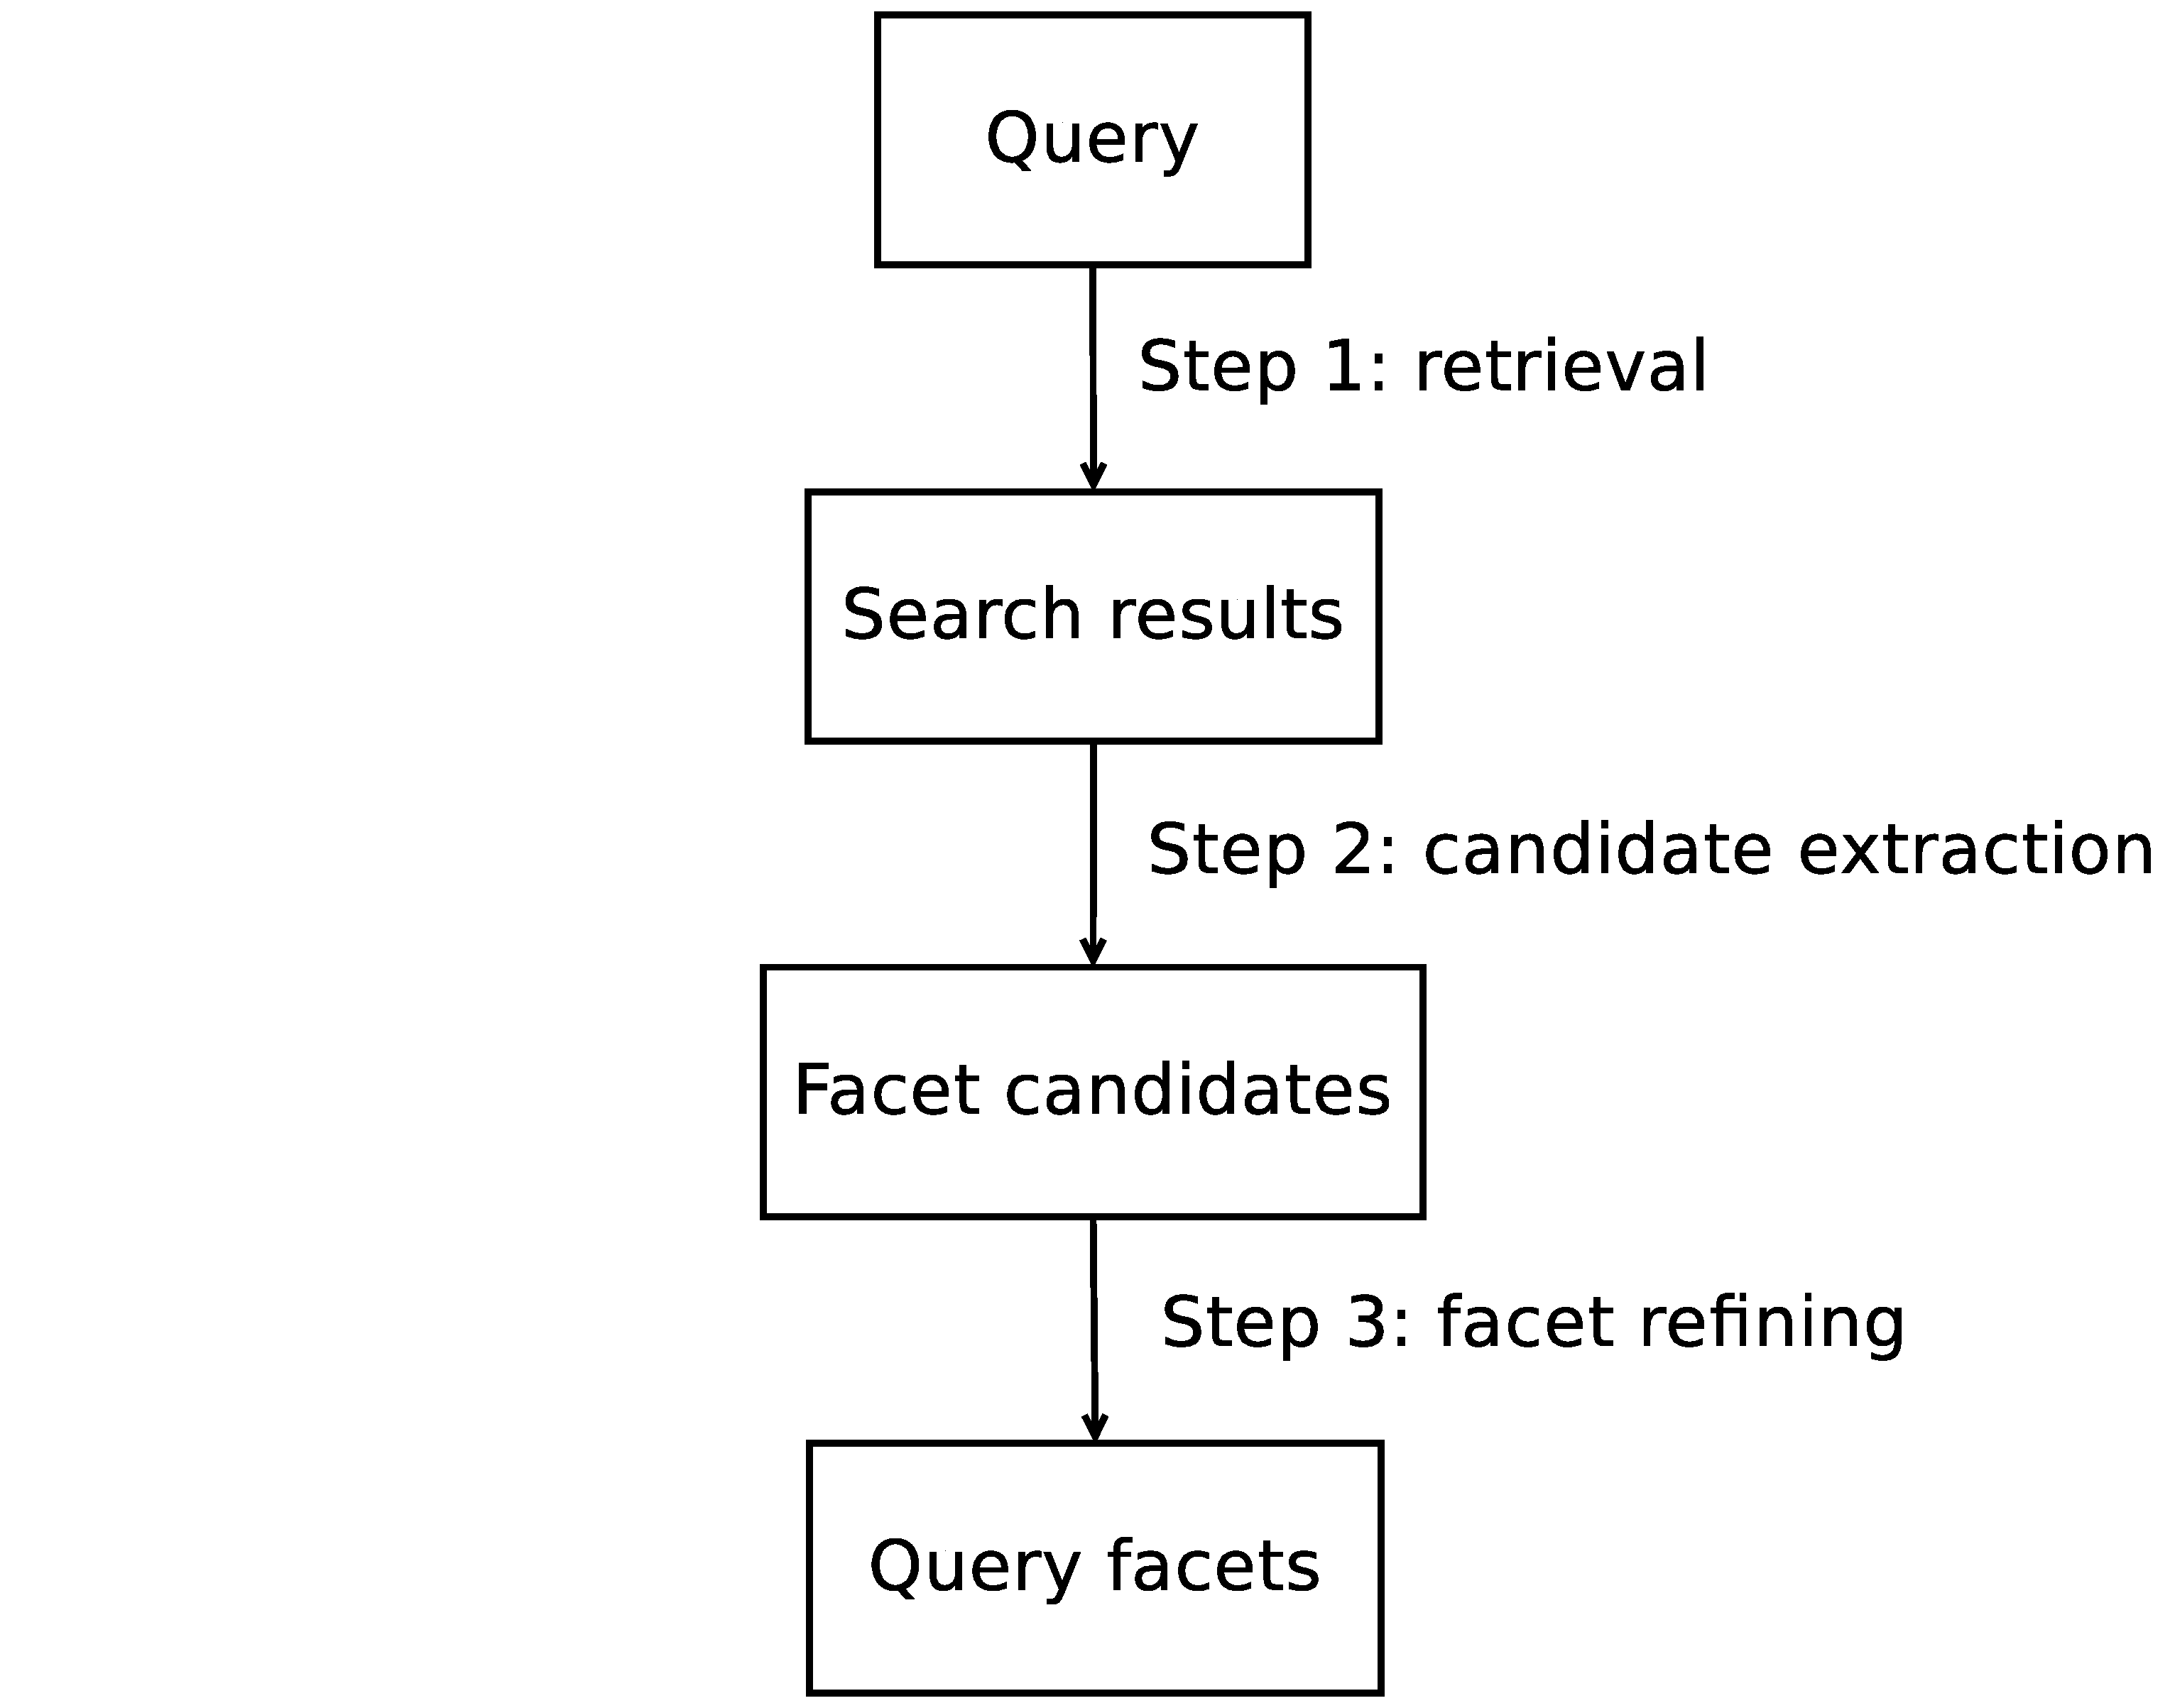
\includegraphics[width=0.85\columnwidth]{drawing/facet-solution.eps}
\caption{Query facet extraction framework}
\label{fig:facet-framework}
\end{figure}
\begin{enumerate}[label={(\arabic*)}]
 \item \textbf{Retrieval}: in the first step, given a query, we retrieve the top search results.
 \item \textbf{Candidate extraction}: in the second step, we extract list structures as facet candidates from the search results based on pre-defined extraction patterns.
 \item \textbf{Facet Refining}: the facet candidates extracted are often very noisy, and cannot be directly used as query facets. In the last step, we refine the candidates to final query facets by re-clustering facets or terms in the candidate set.
\end{enumerate}

We will describe candidate extraction and facet refining in more detail in the next two sections. 

\section{Candidate Extraction}
\label{sec:facet-candidate}
Following \citet{dou2011finding}, we use pattern-based semantic class extraction approach~\cite{shi2010corpus} to extract lists of coordinate terms from search results as facet candidates. In pattern-based semantic class extraction, instances of a semantic class (\eg, instance \concept{AA}, \concept{Delta}, \concept{JetBlue} for class \concept{airlines}) are extracted from textual or webpage corpus based on lexical patterns~\cite{hearst1992automatic,pasca2004acquisition}, HTML patterns~\cite{shinzato2007simple}, or both~\cite{shi2008pattern,zhang2009employing}. For example, the pattern ``\textit{NP} such as \textit{NP}, \textit{NP}, ..., and \textit{NP}'', where \concept{NP} stands for a noun phrase, can be used to extract coordinate terms (as instances) and their hypernyms (as the semantic class) from text. Besides lexical patterns, HTML patterns are often used on HTML documents to extract coordinate terms from some HTML structures, like unordered lists (\ie, <UL>), drop-down lists (\ie, <SELECT>) and 
tables (\ie, <TABLE>). The coordinate terms extracted from each patterns form a candidate for query facets, which we call \textbf{candidate list}.

We apply both of the two types of patterns on the search results to extract candidate lists. These extraction patterns are summarized in Table~\ref{tab:facet-patterns}. We describe them in details in the following two sections.

\begin{table}[ht!]
\centering
\caption{Candidate list extraction patterns. All matched \textit{items} in each pattern are extracted as a candidate list.}
\label{tab:facet-patterns}
\begin{tabular}{|c|l|} \hline
Type& Pattern\\ \hline
Lexical & \textit{item}, \{,\textit{item}$\}^*$, (and|or) \{other\} \textit{item} \\  \hline
\multirow{4}{*}{HTML}
& <select><option>\textit{item}</option>...</select>\\\cline{2-2}
& <ul><li>\textit{item}</li>...</ul>\\\cline{2-2}
& <ol><li>\textit{item}</li>...</ol>\\\cline{2-2}
& <table><tr><td>\textit{item}<td>...</table>\\ \hline
\end{tabular}
\end{table}

\subsection{Lexical Patterns}
We use the following lexical pattern:
\begin{center}
\textit{item}, \{,\textit{item}$\}^*$, (and|or) \{other\} \textit{item} 
\end{center}
We apply the pattern on the textual content (ignoring HTML tags and formatting in the webpage) of the search results, and extract matched \textit{items} as a candidate list. To give an example, for the following sentence,
\begin{center}
\concept{... Mars rovers such as Curiosity, Opportunity and Spirit.}
\end{center}

For this lexical pattern, we also restrict those \textit{items} to be siblings in the parse tree of that sentence in order to improve extraction quality. We use the PCFG parser~\cite{klein2003accurate} implemented in Stanford CoreNLP~\cite{manning2014stanford} for parsing documents.

\subsection{HTML Patterns}
We also extract candidate lists based on several HTML patterns that target list structures in HTML webpages, including drop-down lists, ordered list, unordered list and tables. Table~\ref{tab:facet-html} shows some HTML code examples for these list structures.
\begin{table}[ht!]
\centering
\caption{HTML code examples for drop-down lists (SELECT), ordered lists (OL), unordered lists (UL) and tables (TABLE).} 
\label{tab:facet-html}
\begin{tabular}{|l|} \hline
\textbf{SELECT}: \\
\texttt{<select>}\\
\texttt{<option value=``1''>first class</option>}\\
\texttt{<option value=``2''>business class</option>}\\
\texttt{<option value=``3''>economy class</option>}\\
\texttt{</select>}\\\hline
\textbf{OL}: \\
\texttt{<ol>}\\
\texttt{<li>checked baggage allowance</li>}\\
\texttt{<li>carry on baggage allowance</li>}\\
\texttt{<li>excess baggage allowance</li>}\\
\texttt{</ol>}\\\hline
\textbf{UL}: \\
\texttt{<ul>} \\
\texttt{<li><a href=``courtesy\_bags.aspx''>Courtesy bags</a></li>}\\
\texttt{<li><a href=``dangerous.aspx''>Dangerous goods</a></li>}\\
\texttt{<li><a href="devices.aspx">Electronic devices</a></li>}\\
\texttt{<li><a href="sports.aspx">Sports equipment</a></li>}\\
\texttt{</ul>}\\\hline
\textbf{TABLE}: \\
\texttt{<table>}\\
\texttt{\small<tr><td></td><td>economy</td><td>business</td>first</li>}\\
\texttt{\small<tr>domestic<td>2 bags</td><td>3 bags</td><td>4 bags</td></li>}\\
\texttt{\small<tr>international<td>1 bag</td><td>2 bags</td><td>3 bags</td></li>}\\
\texttt{\small</table>}\\\hline
\end{tabular}
\end{table}

We extract those HTML list structures based on the HTML patterns listed in Table~\ref{tab:facet-patterns}. Note that we do not match the HTML patterns with the HTML code exactly. Instead, we parse the HTML page into objects and extract textual content in the tags that we are interested in. We describe the extraction in details below:
\begin{itemize}
 \item \textbf{SELECT}: For the SELECT tag, we extract textual content in the OPTION tags as a candidate lists. For the example in Table~\ref{tab:facet-html}, we will extract candidate list \{\concept{first class}, \concept{business class}, \concept{economy class}\}.
\item \textbf{OL}: For the OL tag, we extract textual content in the LI tags as a candidate lists. For the example in Table~\ref{tab:facet-html}, we will extract candidate list \{\concept{checked baggage allowance}, \concept{carry on baggage allowance}, \concept{excess baggage allowance}\}.
\item \textbf{UL}: Similarly, for the UL tag, we also extract textual content in the LI tags as a candidate lists. For the example in Table~\ref{tab:facet-html}, we will extract candidate list \{\concept{Courtesy bags}, \concept{Dangerous goods}, \concept{Electronic devices}, \concept{Sports equipment}\}. Note that in this case, when extracting textual content in the LI tags, we ignore other HTML tags/formatting (\ie, \concept{<a>}).
\item \textbf{TABLE}: for HTML tables, following \citet{dou2011finding}, we extract candidate lists from each columns and each rows. For the example in Table~\ref{tab:facet-html}, we will extract 7 candidate lists.
To list a few, \{\concept{economy}, \concept{business}, \concept{first}\} and \{\concept{domestic}, \concept{2 bag}, \concept{3 bags}, \concept{4 bags}\} are extracted from the first two rows. \{concept{domestic}, \concept{international}\} and \{\concept{economy}, \concept{2 bags}, \concept{1 bag}\} are extracted from the first two columns.
\end{itemize}


Ordered lists (OL) and unordered lists (UL) can be nested, as shown in Figure~\ref{fig:nestedlist}. For nested HTML lists, we extract all sibling items from each level. For the example in Figure~\ref{fig:nestedlist}, we will extract two lists,
\{\concept{Coffee}, \concept{Tea}, \concept{Milk}\} and \{\concept{Black tea}, \concept{Green tea}\}.

\begin{figure}[ht!]
\centering
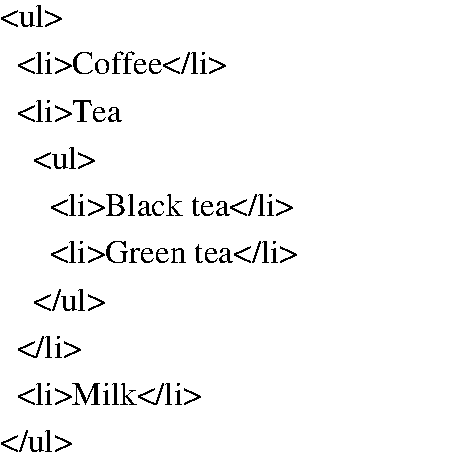
\epsfig{file=drawing/nestedHtmlList.pdf,scale=0.7}
\caption{An example for nested HTML lists.}
\label{fig:nestedlist}
\end{figure}

\subsection{Candidate List Cleaning}
After extracting candidate lists from the top ranked search results, we further clean them as follows:
\begin{enumerate}[label={(\arabic*)}]
 \item First, all the list items are normalized by converting text to lowercase and removing non-alphanumeric characters.
 \item Then, we remove stopwords and duplicate items in each lists.
 \item Finally, we discard all lists that contain only one item or more than 200 items. 
\end{enumerate}

After the cleaning process, we harvest a set of candidate lists, from which we want to build high-quality query facets. 

\section{Facet Refining}
\label{sec:facet-refine}
The candidate lists extracted are usually noisy~\cite{zhang2009employing},
and could be non-relevant to the issued query, therefore they cannot be used directly as query facets. For example, Table~\ref{tab:facet-candidates} shows four candidate lists extracted for the query \concept{baggage allowance}. $L_1$ contains terms that are relevant to \concept{baggage allowance}, but they are not coordinate terms -- \concept{delta}, \concept{france} and \concept{round-trip} are not members of the same class. 
$L_2$ is a valid query facet, but it is incomplete -- another airline \concept{aa} appears in $L_3$. $L_3$ is mixed with different facets, airlines and travel classes. $L_4$ is non-relevant to the query. 
\begin{table}[ht!]
\centering
\caption{Four candidate lists for the query \concept{baggage allowance}}
\label{tab:facet-candidates}
\begin{tabular}{|l|} \hline
 %Candidate facets \\ \hline
$L_1$: delta, france, round-trip\\
$L_2$: delta, jetblue, british airways\\ 
$L_3$: aa, first, business, economy\\
$L_4$: hard to remember, playing it by ear, ...\\
\hline
\end{tabular}
\end{table}

Since the candidate lists are frequently noisy, we need an effective way to refine extracted candidate lists into high-quality query facets. We call this problem \textbf{facet refining}, in which we take a set of candidate lists as input, and want to output high-quality query facets. This facet refining problem is the core issue in query facet extraction, and the focus of our study. Existing query facet extraction models differ in how they refine candidate lists.

One related work about facet refining~\cite{dou2011finding} clusters similarity candidate lists together as query facets (called query dimensions in their original paper), and then ranks/selects clusters and cluster items based on heuristics scores. We find this method is difficult to incorporate features. It also does not have the flexibility of breaking a candidate list into two query facets. We will describe more about this method and other related method for facet refining in Section~\ref{sec:facet-other}. We will also compare these methods with our models in Chapter~\ref{ch:intrinsiceval} and Chapter~\ref{ch:extrinsiceval}.

We instead treat the facet refining problem as a \textbf{selective clustering} problem. In the selective clustering problem, we do not cluster all given items, but only cluster a subset of the items. 
In the case of facet refining, we want to discard noisy terms, and cluster only facet terms in the candidate lists (\eg, \concept{aa}, \concept{delta}, \concept{jetblue}, \concept{british airways}, \concept{first}, \concept{business} and \concept{economy} in Table~\ref{tab:facet-candidates}) into query facets (\eg, \{\concept{aa}, \concept{delta}, \concept{jetblue}, \concept{british airways}\} and \{\concept{first}, \concept{business},\concept{economy}\}). We will present this problem more formally in Section~\ref{sec:facet-formulation}.

To address this problem, we develop a supervised method based on a graphical model, which will be presented in the next section.


\section{Query Faceting Models}
\label{sec:facet-gm}
In this section, we describe query faceting (QF) models, our supervised methods based on a directed graphical model for facet refining. A directed graphical model (or Bayesian network) is a graphical model that compactly represents a probability distribution over a set of variables ~\cite{pearl1988probabilistic}. It consists of two parts: 1) a directed acyclic graph in which each vertex represents a variable, and 2) a set of conditional probability distributions that describe the conditional probabilities of each vertex given its parents in the graph.

We treat facet refining as a selective clustering problem (as described in Section~\ref{sec:facet-refine}), and solve it as a labeling problem, in which we are trying to predict 1) whether a list item is a facet term, and 2) whether a pair of list items is in a same query facet. Then, we used a directed graphical model to exploit the dependences that exist between those labels. Similar to conditional random fields~\cite{lafferty2001conditional}, we directly model the conditional probability $P(y|x)$, where $y$ is the label we are trying to predict and $x$ is the observed data -- list items and item pairs. Thus, it avoids modeling the dependencies among the input variables $x$, and can handle a rich set of features. For our graph model, exact maximum a posteriori inference is intractable; therefore, we approximate the results using two algorithms.

In the rest of this section, we will first describe the facet refining problem more formally in Section~\ref{sec:facet-formulation}, and then present our graphical model in Section~\ref{sec:facet-model}. We will describe how to train and perform inference on the model in Section~\ref{sec:facet-train} and Section~\ref{sec:facet-infer} respectively.

\subsection{Problem Formulation}
\label{sec:facet-formulation}
Before diving into the QF method, we first define the facet refining problem more formally. We use $F=\{t_i\}$ to denote a query facet, consisted by a set of facet terms $t_i$. $\mathcal{F}=\{F_i\}$ denotes the set of query facets for the given query. $T_\mathcal{F}=\bigcup_i{F_i}$ denotes all the facet terms in $\mathcal{F}$. Candidate lists (or candidate facets) are just an imperfect version of query facets, and we substitute ``F'' with ``L'' to denote corresponding variables. $L=\{t_i\}$ denotes a candidate list. $\mathcal{L}=\{L_i\}$ denotes all the candidate lists extracted for the query. $T_\mathcal{L}=\bigcup_i{L_i}$ denotes all list items (or terms) in the candidate lists. Based on the formulation, the facet refining problem is simply to find $\mathcal{F}$ constrained with $T_\mathcal{F} \subseteq T_\mathcal{L}$, given $\mathcal{L}$ (and possibly other resources).

In our query faceting models, facet refining problem was treated as a label prediction problem. It aims to learn and predict jointly 1) whether a list item is a facet term and 2) whether a pair of list items are in the same query facet. We denote the two types of labels as follows. The term/item labels are denoted by $Y=\{y_i\}$, where $y_i = 1\{t_i\!\in\! T_{\mathcal{F}}\}$ is a label indicating whether a list item $t_i$ is indeed a facet term. Here $1\{\cdot\}$ is an indicator function which takes on a value of 1 if its argument is true, and 0 otherwise. The pair labels are denoted by $Z=\{z_{i,j}\}$, where $z_{i,j} = 1\{\exists\, F\!\in\!\mathcal{F}, \, t_{i}\!\in\!F  \wedge  t_{j}\!\in\!F \}$ is a label indicates whether list item $t_i$ and $t_j$ are in a same query facet. Thus, the facet refining problem is now formulated as the problem of predicting labels $Y$ and $Z$.

\subsection{The Graphical Model}
\label{sec:facet-model}
Our supervised method is based on a directed graphical model, aiming to capture the dependencies between the term and pair labels. The graphical model is shown in Figure~\ref{fig:gm}. We further describe it as follows.

\begin{figure}[ht!]
\centering
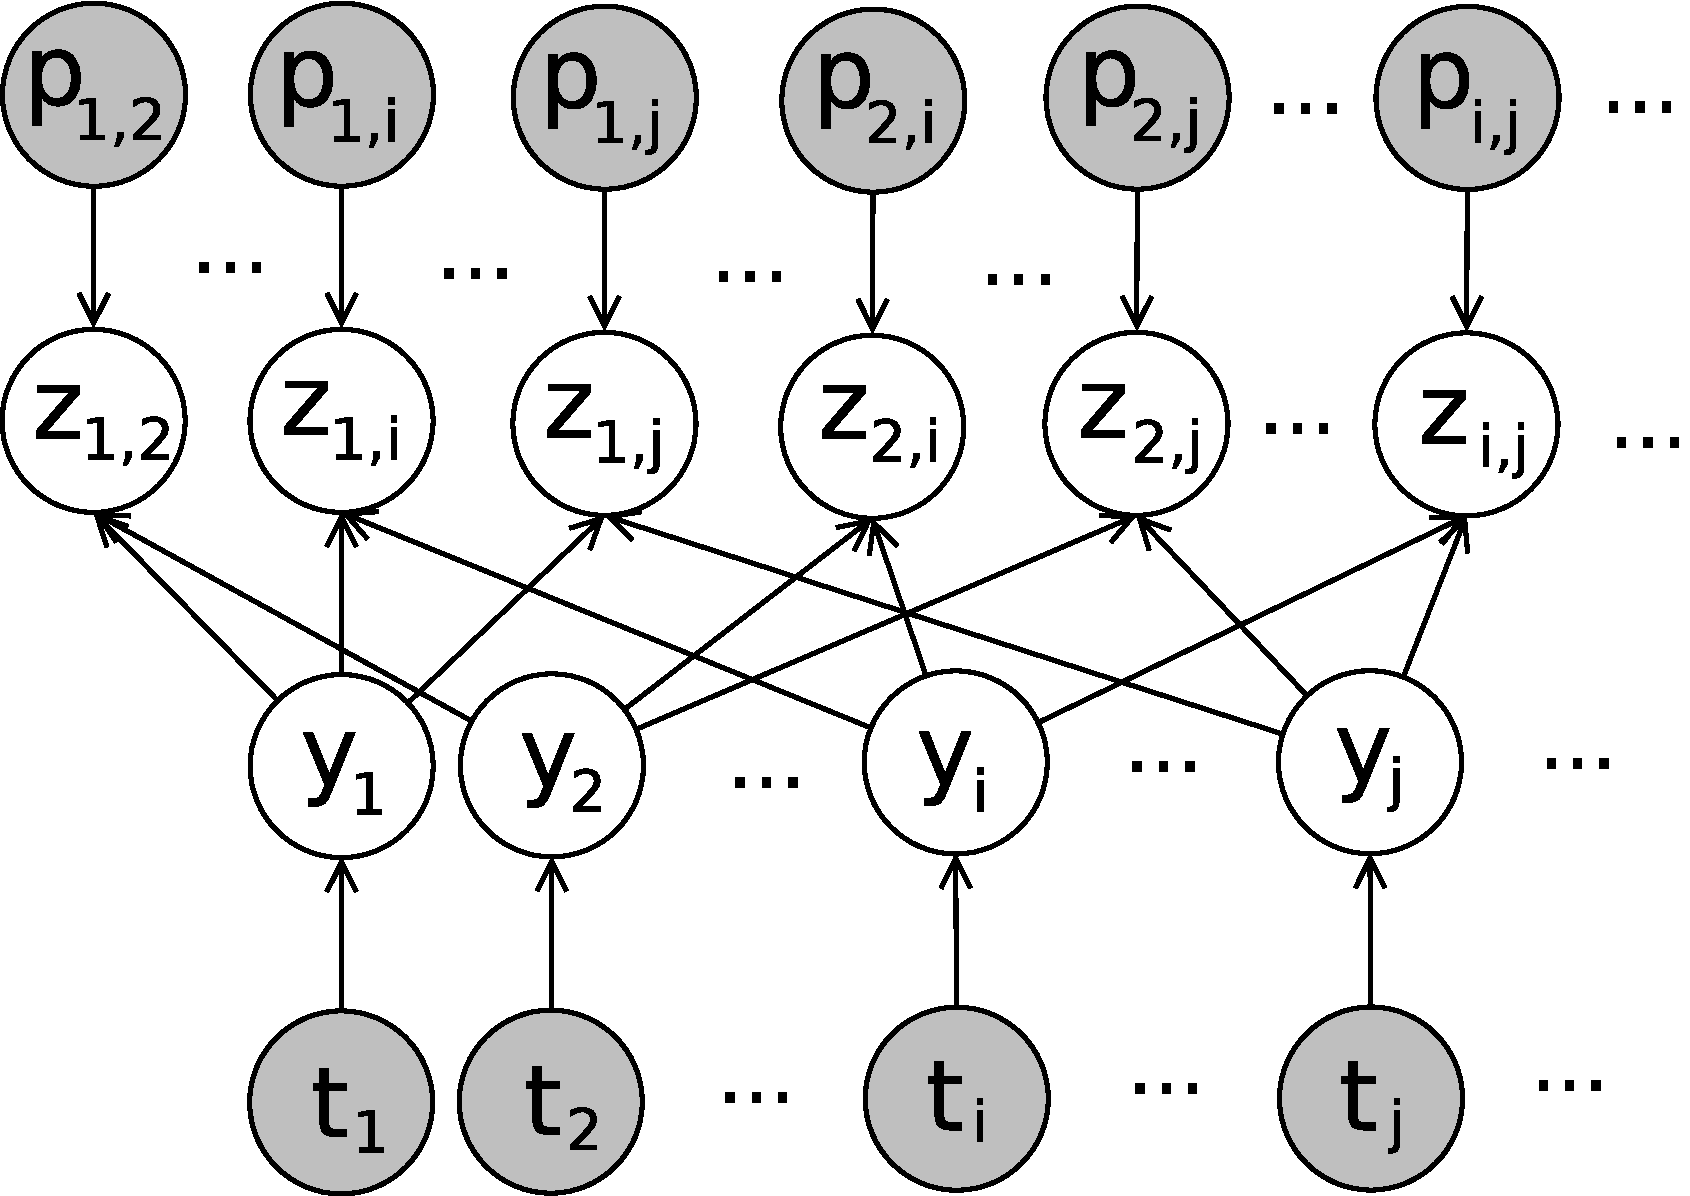
\epsfig{file=drawing/gm.pdf,scale=0.20}
\caption{A graphical model for candidate list data}
\label{fig:gm}
\end{figure}

\subsubsection{The Graph}
First, we describes the four types of variables in the graphical model as follows. We use the formulation described in Section~\ref{sec:facet-formulation}.
\begin{itemize}
 \item list items: $t_i \in T_\mathcal{L}$, as defined before, are all the list items from the extracted candidate lists.
 \item item pairs: $p_{i,j}=(t_i,t_j)$ is simply a short name for term pair $t_i$ and $t_j$. $P_{\mathcal{L}}=\{p_{i,j}|\, t_i,t_j\!\in\!T_{\mathcal{L}}, \, t_i \!\neq\! t_j \}$ are all the item pairs in $T_\mathcal{L}$.
 \item item labels: $y_i \in Y$, as defined before, are all item labels.
  \item pair labels: $z_{i,j} \in Z$, as defined before, are pair labels.
\end{itemize}
List items $t_i$ and item pairs $p_{i,j}$ will be characterized by corresponding features (and will be described in Section~\ref{sec:facet-features}). They are always observed. features (and will be described in Section~\ref{sec:facet-features}). They are always observed. Item labels $y_i$ and pair labels $z_{i,j}$ are what we are trying to predict. In summary, the vertices in our graphical model are $V=T_{\mathcal{L}} \cup P_{\mathcal{L}} \cup Y \cup Z$.

Second, as shown in Figure~\ref{fig:gm}, there are three types of edges in the graph:
\begin{itemize}
 \item edges from each list item $t_i$ to its corresponding labels $y_i$. 
 \item edges that point to each item pair label $z_{i,j}$ from the two corresponding list items $y_i$ and $y_j$.
 \item edges from each item pair $p_{i,j}$ to its corresponding label $z_{i,j}$.
\end{itemize}

\subsubsection{Conditional Probability Distributions}
We use logistic-based conditional probability distributions (CPDs) for variable $y_i$ and $z_{i,j}$, defined as in Equation~\ref{eq:y} and Equation~\ref{eq:z},
\begin{equation}
\label{eq:y}
P(y_i = 1|t_i)=\frac{1}{1+\exp\{-\sum_k{\lambda_k f_k(t_i)}\}},
\end{equation}
\begin{equation}
\label{eq:z}
P(z_{i,j} = 1|p_{i,j},y_i, y_j)=\frac{y_i y_j}{1+\exp\{-\sum_k{\mu_k g_k(p_{i,j})}\}},
\end{equation}
where $f_k$ and $g_k$ are features that characterize a list item and a item pair respectively. $\lambda$ and $\mu$ are the weights associated with $f_k$ and $g_k$ respectively. Compared to a conventional logistic function, Equation~\ref{eq:z} has an extra term, $y_iy_j$, in the numerator. When $y_i=0$ or $y_j=0$, we have $P(z_{i,j}=1|p_{i,j},y_i,y_j)=0$. This means when either of the two list items is not a facet term, the two items can never appear in a query facet together.
When both of the $t_i$ and $t_j$ are facet terms, $P(z_{i,j}=1|p_{i,j},y_i,y_j)$ becomes a conventional logistic function, which models the probability of $t_i$ and $t_j$ being grouped together in a query facet, given the condition that both $t_i$ and $t_j$ are facet term.

\subsubsection{Joint Conditional Probability}
Similar as in conditional random fields~\cite{lafferty2001conditional}, we directly model the joint conditional probability $P(Y,Z|T_{\mathcal{L}},P_{\mathcal{L}})$. Thus, it avoids modeling the dependencies among the input variables $T_{\mathcal{L}},P_{\mathcal{L}}$, and can handle a rich set of features. The joint conditional probability for the graphical model is calculated as
\begin{equation}
\label{eq:joint}
P(Y,Z|T_{\mathcal{L}},P_{\mathcal{L}}) = \prod_{i}{P(y_i|t_i)}\prod_{i,j}{P(z_{i,j}|p_{i,j},y_i, y_j)},
\end{equation}
where the $P(y_i|t_i)$ and $P(z_{i,j}|p_{i,j}, y_i, y_j)$ are defined in Equation~\ref{eq:y} and Equation~\ref{eq:z} respectively.

\subsubsection{Features}
\label{sec:facet-features}
There are two types of features used in our graphical model, term features and (term) pair features. 

\textbf{Item features}, $f_k(t)$ in the graphical model, characterize a single list item in terms of whether the item is a facet term. There are two factors we consider: (1) relevance to the query and (2) quality as a coordinate term. We design a rich set of features to capture the two factors from different perspectives. More specifically, the features we designed are based on different data sources, and based on different types of frequency counts as described in details below.

The different data sources we used include a large web corpus (ClueWeb09), the list item itself, and the top search result webpages. For the top search results, we consider extraction on the following fields/parts:
\begin{itemize}
 \item Content: the textual content of the search result webpages
 \item Title: the title of the search result webpages
 \item List: the candidate lists extracted from the search results. We also consider the candidate lists extracted by each extraction patterns (Section~\ref{sec:facet-candidate}) separately, as we find these patterns are of different extraction qualities \todo{add ref}.
  \begin{itemize}
   \item Text: candidate lists extracted based on the lexical pattern
   \item Ol: candidate lists extracted based on the OL pattern
   \item Ul: candidate lists extracted based on the UL pattern
   \item Select: candidate lists extracted based on the SELECT pattern
   \item Tr: candidate lists extracted based on the TABLE pattern, and extracted by the rows.
   \item Td: candidate lists extracted based on the TABLE pattern, and extracted by the columns.
  \end{itemize}
\end{itemize}

We extract the following types of frequency counts (on the different fields) as features. Note that these frequency-based features are normalized using $log(frequency+1)$ \todo{explain why}.
\begin{itemize}
 \item Termfreq: item/term frequency, the frequency of the list item.
 \item PageFreq: page frequency, the number of search result webpages that contain the list item.
 \item WpageFreq: weighed PageFreq. Each search result webpage count is weighted by its rank, $1/\sqrt{rank}$. This assume that the webpages in the top ranks are more important.
 \item SiteFreq: site frequency, the number of unique websites of the search results that contain the list item. SiteFreq addresses the following problem of PageFreq. Some websites have a fixed template for all of its webpages.  Search results may contains multiple webpages from the same website. In that case, the candidate lists extracted from the template part may repeat multiple times, and be favored by PageFreq unreasonably.  
\end{itemize}

We list all item features in Table~\ref{tab:facet-tfeature}. To capture the relevance of list item (or term) to the query, we use some TF/IDF-based features extracted based on the search result content (Content), title (Title), a webpage corpus (Global corpus), and their combination (Combination). For example, \textit{ContentTermFreq} is the frequency count of the item in the text content of the top $k$ search results. \textit{TitleSiteFreq} is the number of webpages in the top $k$ search results that contain the item in their title. \textit{IDF} is the inverse document frequency of the list item based on a large web page corpus, ClueWeb09\footnote{http://lemurproject.org/clueweb09}. IDF is useful in down-weighting terms that occur frequently in generally, and likely to be less important. We calculate IDF as $IDF(t)=\log{\frac{N-N_{t}+0.5}{N_t+0.5}}$, where $N$ is the total number of documents in the collection, $N_t$ is the number of documents that contain $t$ (document frequency). We also combine different 
features together. For example, \textit{ContentTermFreq.IDF} multiples \textit{ContentTermFreq} with \textit{IDF} (like TF-IDF). \textit{ListTermFreq.ListIDF} multiples \textit{ListTermFreq} with \textit{ListIDF}, where \textit{ListTermFreq} is frequency count of the list item in the candidate lists extracted based on all the patterns. Besides relevance to the 
query and quality as coordinate terms, a facet term should also be succinct. Thus we also use feature \textit{Length}, which count the number of words in the list item.


\begin{table}[h!]
\centering
\caption{Item features}
\label{tab:facet-tfeature}
\begin{tabular}{|c|c|l|l|}
\hline
\multicolumn{2}{|c|}{\textbf{Field/Source}}                &  \textbf{Feature} & \textbf{Description}\\ \hline
\multicolumn{2}{|c|}{\multirow{4}{*}{Content}}   & ContentTermFreq & TermFreq in Content\\ 
\multicolumn{2}{|l|}{}                    &  ContentPageFreq & PageFreq in Content \\  
\multicolumn{2}{|l|}{}                    &  ContentWpageFreq & WpageFreq in Content \\  
\multicolumn{2}{|l|}{}                    &  ContentSiteFreq & SiteFreq in Content \\ \hline  
\multicolumn{2}{|c|}{\multirow{3}{*}{Title}}   & TitleTermFreq & TermFreq in Title  \\ 
\multicolumn{2}{|l|}{}                    &  TitlePageFreq & PageFreq in Title \\  
\multicolumn{2}{|l|}{}                    &  TitleSiteFreq & SiteFreq in Title \\  \hline
		   \multirow{18}{*}{List} & \multirow{3}{*}{ListText} & ListTextTermFreq & TermFreq in ListText \\ 
						 &                   &  ListTextPageFreq & PageFreq in ListText \\ 
					         &                   &  ListTextSiteFreq & SiteFreq in ListText \\ \cline{2-4} 
                  & \multirow{3}{*}{ListOl} & ListOlTermFreq & TermFreq in ListOl \\ 
                  &                   &  ListOlPageFreq      & PageFreq in ListOl\\ 
                  &                   &  ListOLSiteFre       & SiteFreq in List\\ \cline{2-4} 
                  & \multirow{3}{*}{ListUl} & ListUlTermFreq  & TermFreq in ListUl \\ 
                  &                   &  ListUlPageFreq       & PageFreq in ListUl \\ 
                  &                   &  ListUlSiteFreq       & SiteFreq in ListUl \\ \cline{2-4} 
                  & \multirow{3}{*}{ListSelect} & ListSelectTermFreq  & TermFreq in ListSelect \\ 
                  &                   &  ListSelectPageFreq           & PageFreq in ListSelect \\ 
                  &                   &  ListSelectSiteFreq           & SiteFreq in ListSelect \\ \cline{2-4} 
                  & \multirow{3}{*}{ListTr} & ListTrTermFreq  & TermFreq in ListTr\\ 
                  &                   &  ListTrPageFreq       & PageFreq in ListTr \\ 
                  &                   &  ListTrSiteFreq       & SiteFreq in ListTr \\ \cline{2-4} 
                  & \multirow{3}{*}{ListTd} & ListTdTermFreq  & TermFreq in ListTd \\ 
                  &                   &  ListTdPageFreq       & PageFreq in ListTd \\ 
                  &                   &  ListTdSiteFreq       & SiteFreq in ListTd \\ \hline
\multicolumn{2}{|c|}{Term}                &  Length & number of words in the term \\ \hline
\multicolumn{2}{|c|}{\multirow{2}{*}{Global corpus}}   & IDF & inverse document frequency \\ 
\multicolumn{2}{|l|}{}                    &  ListIDF  & IDF in a candidate list collection \\  \hline
\multicolumn{2}{|c|}{\multirow{2}{*}{Combination}}   & ContentTermFreq.IDF &  ContentTermFreq $\times$ IDF \\ 
\multicolumn{2}{|l|}{}                    &  ListTermFreq.ListIDF & ListTermFreq $\times$ ListIDF \\  \hline
\end{tabular}
\end{table}


To capture how likely item $t$ is to be a coordinate terms (or an instance of a semantic class), we use features extracted from candidate lists (List) based on different patterns (ListText, ListOl, ListUl, ListSelect, ListTr, ListTd). For example, \textit{listSelectTermFreq} is the frequency of the list item in the candidate lists extracted based on the SELECT pattern. \textit{listTextPageFreq} is the number of the search result webpages that contains the list item in candidate lists extracted based on the lexical pattern from the webpages. Some list items occur frequently in candidate lists across different queries, such as \textit{home}, \textit{contact us} and \textit{privacy policy}. They are treated as stopwords, and removed from the candidate lists. We also use \textit{listIDF} to cope with this problem, in a similar way as IDF.  \textit{listIDF} is the IDF of a list item in a collection of candidate lists we extracted (see Section~\ref{sec:ie-data}). It is calculated in the same form as \textit{IDF}, 
as $listIDF(t)=\log{\frac{NL-NL_{t}+0.5}{NL_t+0.5}}$, where $NL$ is the total number of candidate lists in the collection,  $NL_t$ is the number of lists contain the list item $t$.


\textbf{Item Pair Features}, $g(p_{i,j})$ in the graphical model, are used to capture how likely a pair of list items should be grouped into a query facet, given that the two list item both are facet terms. We design item pair features based on different types of similarity between the two list items,  listed in Table~\ref{tab:facet-pfeature}. One straightforward feature is to frequency count of the two list items occurring in a same candidate list (\textit{ListCooccur}). Another one is the difference in the length of the list item (\textit{LengthDiff}), which assumes that similar list item should be of similar length. 

\begin{table}[h!]
\centering
\caption{Item pair features. $t_i$ and $t_j$ are an item pair.}
\label{tab:facet-pfeature}
\begin{tabular}{ |l|l| } \hline
  Feature  & Description \\ \hline
  LengthDiff  & Length difference, $|Length(t_i) - Length(t_j)|$ \\
  ListCooccur & Number of candidate lists in which $t_i$, $t_j$ co-occur\\
  TextContextSim & Similarity between text contexts\\
  ListContextSim & Similarity between list contexts\\
\hline
\end{tabular}
\end{table}


Besides these straightforward features, item similarity can also be measured by their context similarity. One common context for a term is the text content surrounding the term~\cite{shi2010corpus}. The feature based on text content similarity is called \textit{textContextSim} in Table~\ref{tab:facet-pfeature}. We build the text context using surrounding words (within 25 words) of the list item in the search result webpages, and represent the text context as a vector of term frequency weights, then we use cosine similarity to calculate \textit{TextContextSim}. Another context we propose in this work is based on the candidate lists extracted, which we call list context. We use list items that appears together with the given list item in a same candidate lists as the list context. An example is given in Table~\ref{tab:facet-listcontext}. In the example, the list context for \concept{Delta} include list item \concept{AA} (twice), \concept{JetBlue} (twice), \concept{Southwest}, and the list context for \concept{
United} include list item \concept{AA}, \concept{JetBlue}, \concept{Southwest}. 
\begin{table}[ht!]
\centering
\caption{A list context example. $L1$, $L2$, $L3$ are three candidate lists. The list context for \concept{Delta} is marked by underline \underline{\textit{item}}, the list context for \concept{United} is marked by double-underline \underline{\underline{\textit{item}}}.}
\label{tab:facet-listcontext}
\begin{tabular}{|l|} \hline
$L_1$: \underline{AA}, \textit{Delta}, \underline{JetBlue} \\
$L_2$: \underline{AA}, \textit{Delta}, \underline{JetBlue},  \underline{Southwest}\\
$L_3$: \underline{\underline{AA}}, \textit{United}, \underline{\underline{JetBlue}}, \underline{\underline{Southwest}}\\ 
\hline
\end{tabular}
\end{table}
Then we can calculate the similarity based on list context in the same way as \textit{TextContextSim} (\ie, using term frequency represent with cosine similar measure). This context similar feature is called \textit{ListContextSim}. \textit{ListContextSim} is to some extent similar to \textit{ListCooccur}, but one advantage of \textit{ListContextSim} is that even if two list items do not co-occur together in a candidate list, they may still have a high \textit{ListContextSim}. For the example in Table~\ref{tab:facet-listcontext}, \concept{Delta} and \concept{United} do not co-occur together in a candidate list, but their list contexts are very similar, and thus they obtain a high \textit{ListContextSim}.


\subsection{Maximum Likelihood Parameter Estimation}
\label{sec:facet-train}
We estimate the parameters $\lambda,\mu$ in the model by maximizing the conditional likelihood of a giving training set. (Later in Chapter~\ref{ch:precision}, we will present another method for parameter estimation by directly maximizing the performing measure.)
The training set for the graphical model can be denoted as
$\{T_{\mathcal{L}}^{(k)},P_{\mathcal{L}}^{(k)},Y^{*(k)},Z^{*(k)}\}$,
where $Y^{*(k)}$, $Z^{*(k)}$ are the ground truth labels for the list items $T_{\mathcal{L}}^{(k)}$ and item pairs $P_{\mathcal{L}}^{(k)}$. (We use superscript ``*'' to denote ground truth labels.)
The conditional probability of the training set can be calculated according to Equation~\ref{eq:train}.
\begin{equation}
\label{eq:train}
P(\lambda,\mu) = \prod_{k}{P(Y^{*(k)},Z^{*(k)}|T_{\mathcal{L}}^{(k)},P_{\mathcal{L}}^{(k)})},
\end{equation}
where $P(Y^{*(k)},Z^{*(k)}|T_{\mathcal{L}}^{(k)},P_{\mathcal{L}}^{(k)})$ is defined in Equation~\ref{eq:joint}. Based on the condition probability, the conditional log-likelihood $l(\lambda, \mu)$, can be calculated as follows,
\begin{equation}
\label{eq:ll}
l(\lambda,\mu) = l_t(\lambda) + l_p(\mu),
\end{equation}
\begin{equation}
\label{eq:lg1}
l_t(\lambda) = \sum_{k}{\sum_{i}{\log P(y_i^{*(k)}|t_i^{(k)})}} - \frac{\sum_{k}{\lambda_k^2}}{2 \sigma^2},
\end{equation}
\begin{equation}
\label{eq:lg2}
l_p(\mu) = \sum_{k}{\sum_{i,j}}{\log P(z_{i,j}^{*(k)}|p_{i,j}^{(k)},y_i^{*(k)},y_j^{*(k)})} -  \frac{\sum_{k}{\mu_k^2}}{2 \gamma^2},
\end{equation}
where the last terms in Equation~\ref{eq:lg1} and Equation~\ref{eq:lg2} are served as regularizers, which penalize large values of $\lambda$, $\mu$. $\sigma$ and $\gamma$ are regularization parameters that control the strength of penalty. 

Notice that, in the train set, for those item pairs $p_{i,j}$ with any of its list item not being a facet term, their labels $z_{i,j}^{*}=0$. According to Equation~\ref{eq:z}, for those item pairs, $\log P(z_{i,j}^{*}|p_{i,j},y_i^{*},y_j^{*})=0$, which makes no contribution to the conditional log-likelihood $l(\mu)$, and thus $l_p(\mu)$ can be simplified as
%\begin{equation}
%\label{eq:lg2x}
%l_p(\mu) = \sum_{T_{\mathcal{L}}}{\sum_{z_{i,j} \in Z'}{\log P(z_{i,j}|p_{i,j},y_i,y_j)}} -  \frac{\sum_{k}{\mu_k^2}}{2 \gamma^2}
%\end{equation}
\begin{equation}
\label{eq:lg2x}
l_p(\mu) = \sum_{k}{\sum_{i,j: y_i^{*(k)}=1, y_j^{*(k)}=1}}{\log P(z_{i,j}^{*(k)}|p_{i,j}^{(k)},y_i^{*(k)},y_j^{*(k)})} -  \frac{\sum_{k}{\mu_k^2}}{2 \gamma^2},
\end{equation}
where the $i,j$ now indexes only item pairs with both of its list items being facet terms (\ie,$y_i^{*(k)}=1, y_j^{*(k)}=1$).

We can see that Equations~\ref{eq:lg1} and \ref{eq:lg2x} are exactly the same as log-likelihoods for two separated logistic regressions. In fact, Equation~\ref{eq:lg1} learns a logistic regression model for whether a list item is a facet term, and Equation~\ref{eq:lg2x} learns a logistic regression model for whether two facet terms should be grouped together.
The parameter $\lambda$ and $\mu$ can be learned by maximizing the log-likelihood using gradient descent, exactly same as in logistic regression.
\todo{add gradient equations}
%Its partial derivatives can be calculated as follows,
%\begin{equation*}
%\label{eq:lg1p}
%\frac{\partial l(\lambda,\mu)}{\partial \lambda_k}  = \sum_{T_{\mathcal{L}}}{\sum_{y_i \in Y}{\left( y_i-P(y_i=1|t_i) \right) f_k(t_i)}} 
%- \frac{\lambda_k}{\sigma^2}
%\end{equation*}
%\begin{equation*}
%\label{eq:lg2p}
%\frac{\partial l(\lambda,\mu)}{\partial \mu_k}  = \sum_{T_{\mathcal{L}}}{\sum_{z_{i,j} \in Z'}{\left( z_{i,j}- %P(z_{i,j}=1|p_{i,j},y_i,y_j) \right) g_k(p_{i,j})}} 
%- \frac{\mu_k}{\gamma^2}
%\end{equation*}

\subsection{Inference}
\label{sec:facet-infer}
When given a new labeling task, we could perform maximum a posteriori inference -
compute the most likely labels $Y, Z$ by maximizing the joint conditional probability $P(Y,Z|T_{\mathcal{L}},P_{\mathcal{L}})$.
After that, the query facet set $\mathcal{F}$ can be easily induced from the labeling $Y, Z$.
(Collect list items with $y_i=1$ as facet terms, and group any two of them into a query facet if the corresponding $z_{i,j}=1$.)
Note that the graphical model we designed does not enforce the labeling to produce strict partitioning for facet terms.
For example, when $Z_{1,2}=1$, $Z_{2,3}=1$, we may have $Z_{1,3}=0$.
Therefore, the labeling results may induce an overlapping clustering.
Unfortunately, this optimization problem is NP-hard, which can be proved by a reduction from the Ising model~\cite{barahona1982computational}.

To facilitate developing solutions, we add the strict partitioning constraint that each facet term belongs to exactly one query facet. Also, to directly produce the query facets, instead of inducing them after predicting labels, we rephrase the optimization problem as follows. First, we use the following notations for log-likelihoods,\todo{clear up the equations}
\begin{eqnarray*}
 s_t(t_i) &=& \log P(y_i=1|t_i)      \nonumber \\
  \overline{s_t}(t_i)&=&\log \left( 1-P(y_i=1|t_i) \right) \nonumber \\
 s_p(t_i, t_j)&=&\log P(z_{i,j}=1|p_{i,j},y_i=1,y_j=1) \nonumber \\
  \overline{s_p}(t_i, t_j)&=&\log\left(1-P(p_{i,j}=1|p_{i,j},y_i=1,y_j=1)\right) \nonumber
\end{eqnarray*}
Using the notations above, the log-likelihood $l(\mathcal{F})$ for a particular query facet set $\mathcal{F}$ formed from $\mathcal{L}$ can be written as 
\begin{eqnarray}
\label{eq:target}
l(\mathcal{F}) &=&l_t(\mathcal{F}) + l_p(\mathcal{F}) \nonumber\\
l_t(\mathcal{F}) &=& \sum_{t\in T_\mathcal{F}}{s_t(t_i)}+\sum_{t\not\in T_\mathcal{F}}{\overline{s_t}(t_i)} \nonumber \\
l_p(\mathcal{F}) &=&\sum_{F \in \mathcal{F}}{\sum_{t_i,t_j \in F}{s_p(t_i,t_j)}} 
+ \sum_{\substack{F, F' \\ \in \mathcal{F}}}{\sum_{\substack{t_i \in F, \\ t_j \in F'}}{\overline{s_p}(t_i,t_j)}}
\label{eq:targetp}
\end{eqnarray}
In the right hand side of Equation~\ref{eq:targetp}, the first term  is the intra-facet score, which sums up $s_p(\cdot, \cdot)$ for all the item pairs in each query facet. The second term is the inter-facet score, which sums up the $\overline{s_p}(\cdot,\cdot)$ for each item pair that appears in different query facets. Then the optimization target becomes $\mathcal{F}=\arg\max_{\mathcal{F}\in\mathfrak{F}}{l(\mathcal{F})}$, where $\mathfrak{F}$ is the set of all possible query facet sets that can be generated from $\mathcal{L}$ with the strict partitioning constraint.

This optimization problem, however, is still NP-hard, which can be proved by a reduction from the Multiway Cut problem~\cite{bansal2002correlation}.
Therefore, we propose two algorithms, \textbf{QFI} and \textbf{QFJ}, to approximate the results.

\todo{add proof for NP-hardness}
\subsubsection{QFI}
QFI approximates the results by predicting whether a list item is a facet term and whether two list items should be grouped in a query facet independently, which is accomplished two phases.
In the first phase, QFI selects a set of list items as facet terms according to $P(y_i|t_i)$.
In this way, the algorithm predicts whether a list item $t_i$ is a facet term independently, ignoring the dependences between $y_i$ and its connected variables in $Z$.
In our implementation, we simply select list items $t_i$ with  $P(t_i)> w_{min}$ as facet terms. (For convenience, we use $P(t_i)$ to denote $P(y_i=1|t_i)$.)
In the second phase, the algorithm clusters the facet terms $T_\mathcal{F}$ selected in the first phase into query facets, according to $P(t_i,t_j)$. ($P(t_i, t_j)$ is used to denote $P(z_{i,j}=1|p_{i,j},y_i=1,y_j=1)$).
Many clustering algorithm can be applied here, using $P(t_i,t_j)$ as the distance measure.
For our implementation, we use a cluster algorithm based on WQT~\cite{dou2011finding}, because it considers the importance of nodes while clustering.
We use $P(t_i)$ as the measure for facet term importance, and $d_t(t_i,t_j)=1-P(t_i, t_j)$ as the distance measure for facet terms. The distance between a cluster and a facet term is computed using complete linkage distance, $d_f(F,t)=max_{t' \in F}{d(t, t')}$, and the diameter of a cluster can be calculated as $dia(F)=\max_{t_i,t_j\in F}{d_t(t_i,t_j)}$. The algorithm is summarized in Algorithm~\ref{alg:qfi}. It processes the facet terms in decreasing order of $P(t)$. For each facet term remaining in the pool, it builds a cluster by iteratively including the facet term that is closest to the cluster, until the diameter of the cluster surpasses the threshold $d_{max}$.
\begin{algorithm}[ht!]
 \caption{WQT for clustering facet term used in QFI}
\label{alg:qfi}
\begin{algorithmic}[1]
  \Require $T_{\mathcal{F}}, P(t), d_f(F,t), dia(F), d_{max}$
  \Ensure $\mathcal{F}=\{F\}$
  \State $T_{pool} \leftarrow \mathcal{F}$
  \Repeat
    \State $t \leftarrow \arg\max_{t\in T_{pool}}{P(t)}$
    \State $F \leftarrow \{t\}$
    \State iteratively include facet term $t' \in T_{pool}$ that is closest to $F$, according to $d_f(F,t')$, until the diameter of the cluster, $dia(F)$, surpasses the threshold $d_{max}$.
    \State $\mathcal{F} \leftarrow \mathcal{F} \cup \{F\}$, $T_{pool} \leftarrow T_{pool} - F$
  \Until $T_{pool}$ is empty
  \State \Return $\mathcal{F}$
\end{algorithmic}
\end{algorithm}


\subsubsection{QFJ}
QFI finds query facets based on the graphical model by performing inference of $y_i$ and $z_{i,j}$ independently.
The second algorithm, QFJ, instead tries to perform joint inference by approximately maximizing our target $l(\mathcal{F})$ with respect to  $y_i$ and $z_{i,j}$ iteratively.
The algorithm first guesses a set of list items as facet terms.
Then it clusters those facet terms by approximately maximizing $l_p(\mathcal{F})$, using a greedy approach. 
After clustering, the algorithm checks whether each facet term ``fits'' in its cluster, and removes those that do not fit.
Using the remaining facet terms, the algorithm repeats the process (clustering and removing outliers) until convergence.

QFJ is outlined in Algorithm~\ref{alg:qfj}. The input to the algorithm are the candidate list item set $T_{\mathcal{L}}$,
and the log-likelihoods $l(\mathcal{F})$, $l_p(\mathcal{F})$.
In the first step, we select top $n$ list items according to $s_t(t)$ as the initial facet terms, because it is less sensitive to the absolute value of the log-likelihood.
In our experiment, $n$ is set to 1000 to make sure most of the correct facet terms are included.
Then, the algorithm improves $l(\mathcal{F})$ by iteratively performing functions \textproc{Cluster} and \textproc{RemoveOutliers}.
\textproc{Cluster} performs clustering over a given set of facet terms.
In step 10 to 12, it puts each facet terms into a query facet by greedily choosing the best facet, or creates a singleton for the list item, according to the resulting log-likelihood, $l_p(\mathcal{F})$.
%In step 5, $\Delta_{1}(F)$ is the difference between $l(\mathcal{F})$'s changes of adding the list item $t$ to $F$ and creating a singleton for $t$.
We choose to process these list items in decreasing order of $s_t(t)$, because it is more likely to form a good query facet in the beginning by doing so.
\textproc{RemoveOutliers} removes facet terms according to the joint log-likelihood $l(\mathcal{F})$.
In step 20 to 22, it checks each facet term to see if it fits in the facet, and removes outliers.
$F'$ is the set of facet terms the algorithm selected when processing each facet $F$.
%In step 7 to 12, the algorithm chooses the best option for $t$ to maximize the log-likelihood $l(\mathcal{F})$. The list items we select from step 2 may contain ``bad'' facet terms. In step 14 to 24, the algorithm tries to delete those mistakes by locally optimize $l(\{F\})$ for each query facet $F$ formed. For each facet $F$, it consider whether each list item in the list should be delete or not. In step 15, $F'$ is the set of list items that we think should be kept after processing. $\Delta_2$ is the difference between $l(\{F'\})$'s changes of not including $t$ in $F'$ and including $F'$.


\begin{algorithm}[ht!]
 \caption{QFJ}
\label{alg:qfj}
\begin{algorithmic}[1]
  \Require $T_{\mathcal{L}}=\{t\}, l, l_p$
  \Ensure $\mathcal{F}=\{F\}$
  \State $T_\mathcal{F} \leftarrow$ top $n$ list items from $T_{\mathcal{L}}$ according to $s_t(\cdot)$ 
  \Repeat
  \State $\mathcal{F}\leftarrow$ \Call{Cluster}{$T_{\mathcal{F}},l_p$}
  \State $T_\mathcal{F}\leftarrow$ \Call{RemoveOutliers}{$\mathcal{F},l$}
  \Until converge
  \State \Return $\mathcal{F}$
  \State
  \Function{cluster}{$T_\mathcal{F}, l_p$}
    \State $\mathcal{F} \leftarrow \emptyset$ 
    \For {each $t \in T_\mathcal{F}$ in decreasing order of $s_t(t)$}
      \State Choose to put $t$ into the best facet in $\mathcal{F}$ or add $t$ as a singleton into $\mathcal{F}$, whichever that has the highest resulting $l_p(\mathcal{F})$.
      %\For {each $F \in \mathcal{F}$}
	%\State $\Delta_{1}(F)\leftarrow \sum_{t' \in F}{\left(s_p(t,t')-\overline{s_p}(t,t')\right)}$ 
      %\EndFor
      %\If{$\max_{F}{\Delta_{1}(F)} < 0$}
	%\State $F' \leftarrow \{t\}, \mathcal{F}\leftarrow \mathcal{F} \cup \{F'\}$
      %\Else
      %\State find the best facet, $F_{best} \leftarrow \arg\max_F{\Delta_{1}(F,t)}$
      %\State add $t$ to the facet in $\mathcal{F}$, $F_{best} \leftarrow F_{best} \cup \{t\}$
      %\EndIf
    \EndFor 
  \State \Return $\mathcal{F}$
  \EndFunction 
  \State
\Function{RemoveOutliers}{$\mathcal{F},l$}
  \State $T_\mathcal{F}\leftarrow$ all facet terms in $\mathcal{F}$
  \For {each $F \in \mathcal{F}$}
    \State $F'=\emptyset$
    \For {each $t \in F$ in decreasing order of $s_t(\cdot)$}
      \State choose to add $t$ into $F'$ or not, whichever has the highest resulting $l(\{F'\})$
      \State if not, $T_\mathcal{F}\leftarrow \mathcal{F} - \{t\}$
      %\State $\Delta_{2} = \overline{s_t}(t) - s_t(t) - \sum_{t'\in F'}{s_p(t,t')} $
      %\If {$\Delta_{2} > 0$}
	%  \State remove $t$ from the facet in  $\mathcal{F}$, $F \leftarrow F - \{t\}$
      %\Else
	%  \State $F' \leftarrow F' \cup \{t\}$
      %\EndIf
    \EndFor
  \EndFor
  \State \Return  $T_\mathcal{F}$
\EndFunction 
  \State \Return $\mathcal{F}$
\end{algorithmic}
\end{algorithm}

\subsection{Ranking Query Facets}
The output of QFI and QFJ is a query facet set $\mathcal{F}$. To produce ranking results, we defined a score for a query facet as $score_F(F)=\sum_{t \in F}{P(t)}$, and rank the query facets according to this scoring, in order to present more facet terms in the top. Facet terms within a query facet are ranked according to $score_t(t)=P(t)$. We leave the investigation for more sophisticated ranking models as future work.

\section{Other Approaches}
\label{sec:facet-other}
In this section, we describe two alternative method for facet refining. They are used as baselines in our experiments. 

\subsection{QDMinder}
\citet{dou2011finding} developed QDMiner/QDM for query facet extraction, which appears to be the first work that addressed the problem of query facet extraction.
To solve the problem of finding query facets from the noisy candidate lists extracted, they used an unsupervised clustering approach.
It first scores each candidate list by combining some TF/IDF-based scores.
The candidate lists are then clustered with bias toward important candidate lists, 
using a variation of the Quality Threshold clustering algorithm~\cite{heyer1999exploring}.
After clustering, clusters are ranked and list items in each clusters are ranked/selected based on some heuristics.
Finally, the top $k$ clusters are returned as results.
%They applied clustering on the candidates lists, and ranked/selected clusters and list items in those clusters based on some heuristics.
This unsupervised approach does not gain by having human labels available.
Also, by clustering lists, they lose the flexibility of breaking a candidate list into different query facets.

\subsection{Topic modeling}
In semantic class extraction, \citet{zhang2009employing} proposed to use topic models 
to find high-quality semantic classes from a large collection of extracted candidate lists.
Their assumption is, like documents in the conventional setting, candidate lists are generated by a mixture of hidden topics, which are the query facets in our case. pLSA and LDA are used in their experiments.
We find this approach can be directly used for finding query facets from candidate lists.
The major change we need to make is that: in semantic class extraction, topic modeling is applied globally on the candidate lists (or a sample of them) from the entire corpus; in query facet extraction, we apply topic modeling only on the top $k$ search results $\mathcal{D}$, assuming the coordinate terms in $\mathcal{D}$ are relevant to the query.
Then, the topics are returned as query facets, by using the top $n$ list items in each topic (according to the list item's probability in the topic).
Though this topic modeling approach is more theoretically motivated, it does not have the flexibility of adding different features to capture different aspects such as query relevance.

\section{Summary}
In this chapter, we developed query facet extraction, which extracts facets for a given query from its search results. We developed a supervised approach based on a graphical model to recognize facets from the noisy candidates found. The graphical model learns how likely a candidate term is to be a facet term as well as how likely two terms are to be grouped together in a query facet, and captures the dependencies between the two factors. We proposed two algorithms (\QFI and \QFJ) for approximate inference on the graphical model since exact inference is intractable. Compared with other existing methods, our models can easily incorporate a rich set of features, and learn from available labeled data.

To evaluate our models, in the next chapter, we will develop an intrinsic evaluation method that compares extracted facets with human created ones.

\chapter{Intrinsic Evaluation} 
\label{ch:intrinsiceval}
\section{Introduction}
Intrinsic evaluation is to evaluate the quality of query facet generation itself. We perform intrinsic evaluation by comparing system generated query facets with ``gold standard'' query facets. Note that this evaluation can be easily extended for evaluating new models (\ie, compare the query facets generated by the new models with the existing ``gold standard'' query facets  collected before). Later, in Chapter~\ref{ch:extrinsiceval}, we will carry out an extrinsic evaluation that evaluates the quality of generated facets by their utility in assisting search.

The ``gold standard'' query facets are constructed by human annotators and used as the ground truth to be compared with facets generated by different systems. The facet annotation is usually done by first pooling facets generated by the different systems. Then annotators are asked to group or re-group terms in the pool into preferred query facets, and to give ratings for each of them regarding how useful or important the facet is.


In intrinsic evaluation, the quality of generated query facets can be measured from two aspects. (1) How well does the model generate/find correct facet terms. This can be measured by standard classification measures, such as precision and recall. (2) How well does the model groups facet terms correctly. This can be measured by standard clustering measures, such as F-measures for clustering, Purity and Normalized Mutual Information.

However, a single performance measure that combines the different aspects can be desirable in many cases. First, such a single measure provides an overall measurement for effectiveness, which is often necessary for comparing different models. Second, such a single measure can be used for tuning or training models. For example, in Chapter~\ref{ch:precision}, we propose a method that directly using a performance measure as the training object. 

To combine the two evaluation aspects, we design a new measure called $PRF_{\alpha,\beta}$~\cite{kong2013extracting}. $PRF_{\alpha,\beta}$ combines $TP$, $TR$ and $PF$ using weighted harmonic mean, where $TP$, $TR$ and $PF$ are precision and recall for facet terms, and the F1 measure for facet term clustering. Parameters $\alpha$ and $\beta$ can be used to adjust the emphasis of the three factors for different applications.

However, $PRF_{\alpha,\beta}$ does not directly account for facet ranking performance. Dou et al.~\cite{dou2011finding} used some variations of nDCG to evaluate facet ranking. In the nDCG variation measures, system facets are mapped to truth facets, and assigned ratings according to their mapped truth facets. Then the ranked system facets are evaluated using nDCG, with the discounted gain further weighted by the precision and recall of the system facet and mapped truth facet. However, we will show that this metric can be problematic in some cases.

In the experiments of this chapter, we perform intrinsic evaluation on the different query facet extraction models described in Chapter~\ref{ch:facet}. The experimental results show that our supervised method (QFI and QFJ) proposed in Chapter~\ref{ch:facet} significantly outperforms other unsupervised methods, suggesting that query facet extraction can be effectively learned.

In the rest of this chapter, we will first described how we collect data and perform facet annotation for intrinsic evaluation in Section~\ref{sec:ie-data}. Then, we will describe different evaluation metrics in Section~\ref{sec:ie-metrics}, including $PRF_{\alpha,\beta}$ and other existing measures. We will present our experiments for comparing different query facet extraction models in Section~\ref{sec:ie-exp}, followed by conclusions in Section~\ref{sec:ie-conclusions}. 
%The work in this chapter is completed and published~\cite{kong2013extracting}.


\section{Data} \label{sec:ie-data}
\subsection{Query}
We constructed a pool of 232 queries from different sources, including random samples from a query log, TREC 2009 Web Track queries~\footnote{http://trec.nist.gov/data/web/09/wt09.topics.queries-only}, example queries appearing in related publications~\cite{xue2011topic,wang2009mining} and queries generated by our annotators.
Annotators were asked to select queries that they are familiar with from the pool for annotating.
Overall, we collect annotations for 100 queries (see Table~\ref{tab:queries}).

\begin{table}[ht!]
\vspace{-3mm}
\centering
\caption{Query statistics}
\label{tab:queries}
\begin{tabular}{|r|r|r|} \hline
Source& \#queries& \#queries \\ 
& \ collected& \  annotated\\ \hline
query log & 100 & 30\\ 
related publications & 20 & 10\\ 
TREC 2009 Web Track & 50 & 20\\ 
annotators generated & 62 & 40\\ \hline
sum & 232 & 100\\ \hline
\end{tabular}
\end{table}	

\subsection{Search Results}
For each query, we acquire the top 100 search results from Bing\footnote{a commercial web search engine, http://www.bing.com/}. 
A few search results were skipped due to crawl errors, or if they were not HTML Web pages.
For the 232-query set, we crawled 22,909 web pages, used for extracting feature $listIDF$ described in Section~\ref{sec:facet-features}. For the 100 annotated queries, the average number of crawled web pages is 98.7, the minimum is 79, both the maximum and the median are 100.

\begin{figure}[ht!]
\centering
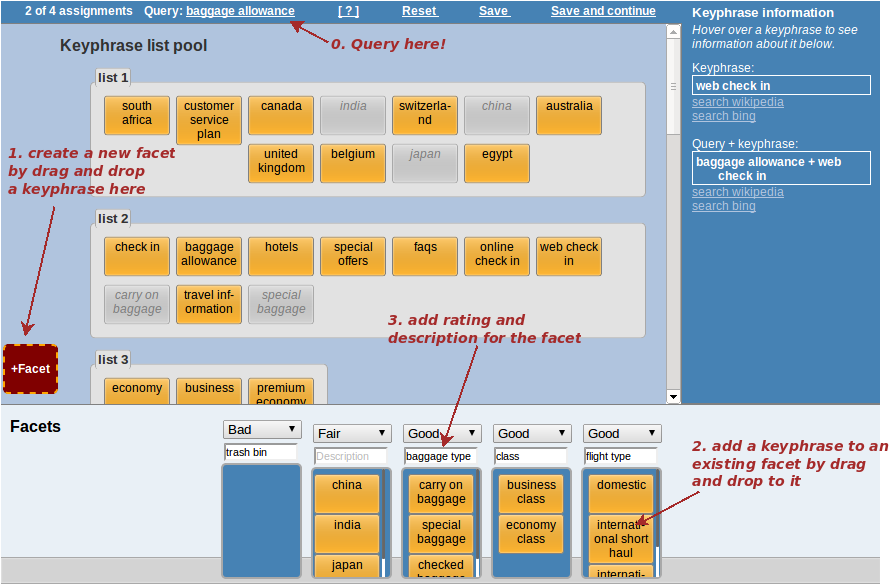
\epsfig{file=figure/facet-annotation-ui.png,scale=0.45}
%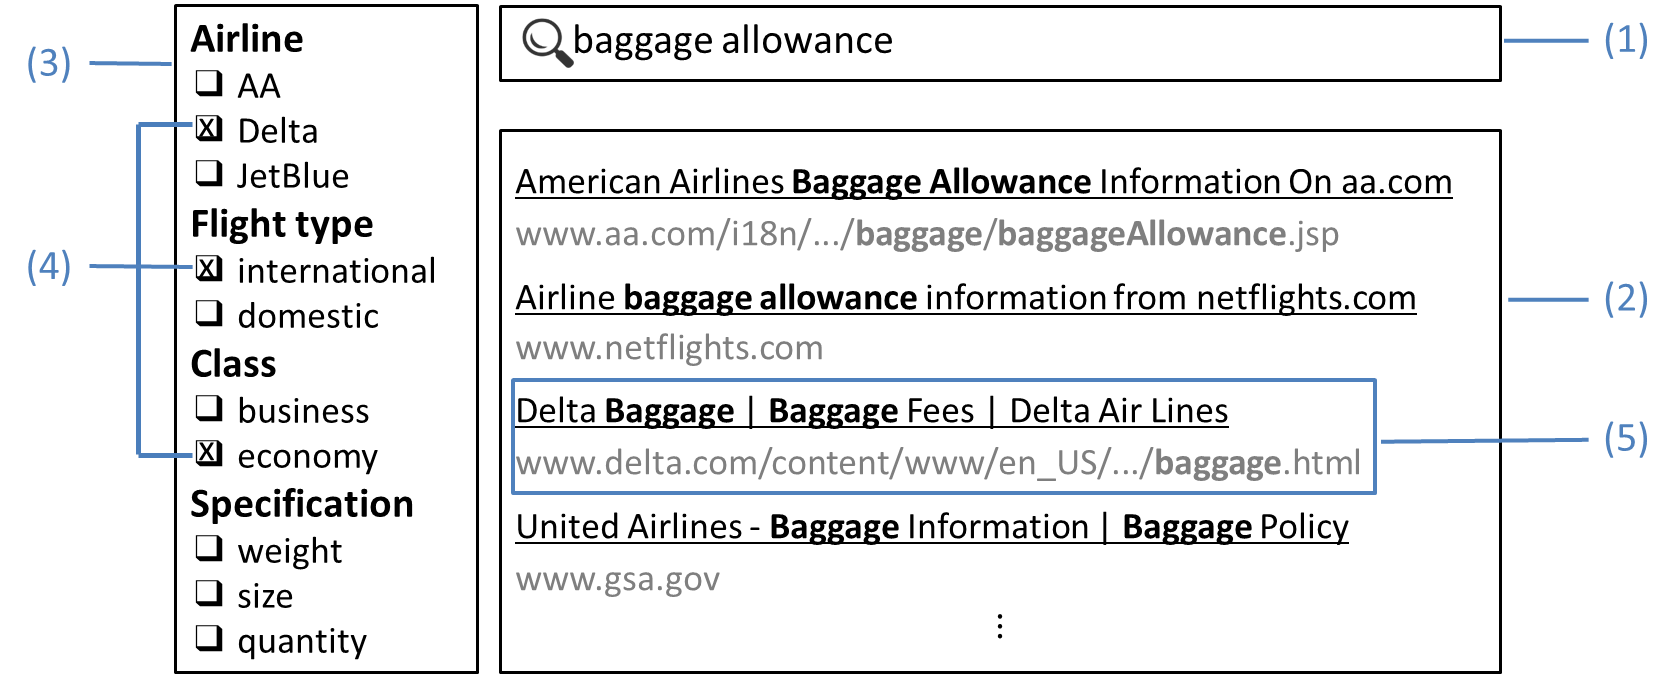
\includegraphics[scale=0.45]{figure/fws-example.png}
\caption{Annotation interface for query facet annotation.}
\label{fig:facet-annotation}
\end{figure}

\subsection{Query facet annotations}
\todo{include inter-annotator agreement on facts}
\todo{move annotation method in to an individual section, and talk about annotation trials.}
We asked human annotators to construct query facets as ground truth, using the annotation interface shown in Figure~\ref{fig:facet-annotation}.
For each query, we first constructed a pool of terms by aggregating facet terms in the top 10 query facets generated by different models (corresponding to ``keyphrase list pool'' in Figure~\ref{fig:facet-annotation}), including two runs from QDM, one run from each of pLSA and LDA using top 10 list items in each query facets, and one run for our graphical model based approach. 
Then, annotators were asked to group terms in the pool into query facets for each query they selected (corresponding to step 1 and 2 in Figure~\ref{fig:facet-annotation}).
Finally, the annotator was asked to give a rating for each constructed query facet, regarding how useful and important the query facet is (corresponding to step 3 in Figure~\ref{fig:facet-annotation}). The rating scale of good=2/fair=1 is used. 

We recruited 17 human annotators (5 females and 12 males), with 16 graduate students (computer science major) and 1 undergraduate student from our university. Prior to the actual annotation task, annotators were assigned a training session (using another query that is not in the data set) to get familiar with the task and annotation interface.

There are 50 query facets pooled per query, with 224.8 distinct facet terms per query. Annotation statistics for the good and fair facets, as well as the pooled facet, are given in Table~\ref{tab:annotations}. The table shows average number of facet terms per query, average number of query facets per query, and average number of facet terms per facet, for each categories (fair, good, and pooled facets).
\begin{table}[ht!]
\centering
\caption{Annotation statistics}
\label{tab:annotations}
\begin{tabular}{|l|r|r|r|} \hline
& fair & good & pooled\\ \hline
\#terms per query & 26.6 & 55.8 & 224.8\\ 
\#facets per query & 3.1 & 4.8 & 50.0 \\ 
\#terms per facet & 8.6 & 11.6 & 8.8 \\ \hline
\end{tabular}
\end{table}

\section{Metrics} 
\label{sec:ie-metrics}
Query facet extraction can be evaluated from different aspects. A good system should select ``correct'' facet terms from all the list items, therefore we use standard classification metrics, such as precision, recall and F-measures. A good system should also group those facet term correctly (i.e., in the same way as the annotators), therefore we use standard clustering metrics, such as F-measures for clustering, Purity and Normalized Mutual Information. To combine the different evaluation aspects, we design a new measure for this particular task.
\subsection{Notations} \label{sec:evalmetrics}
We continue to use notations defined in Section~\ref{sec:facet-formulation} for a query facet ($F$), a query facet set ($\mathcal{F}$) and the set of all facet terms ($T_{\mathcal{F}}$) in a query facet set. We use ``$*$'' to distinguish between system generated results and human labeled results, which we used as ground truth.
For example, $\mathcal{F}$ denotes the system generated query facet set, and $\mathcal{F}^*$ denotes the human labeled query facet set.
For convenience, we use $T$ to denote $T_{\mathcal{F}}$ in this Chapter, omitting subscript $\mathcal{F}$.
$T^*$ denotes all the facet terms in human labeled query facet set.
We use $r_{F^*}$ to denote the rating score for a human labeled facet $F^*$.

\subsection{Effectiveness in finding facet terms}
\label{sec:intrinsic-tmeasures}
One aspect of query facet extraction evaluation is how well a system finds facet terms. This can be evaluated using standard classification metrics as follows,
\begin{itemize}
 \item facet term precision: $T\!P=\frac{|T \cap T^*|}{|T|}$
 \item facet term recall: $T\!R=\frac{|T \cap T^*|}{|T^*|}$
 \item facet term F1: $T\!F=\frac{2|T \cap T^*|}{|T|+|T^*|}$
\end{itemize}
where the \concept{T} in measure names $T\!P$, $T\!R$, $T\!F$ stands for facet \emph{term}. It is used to distinguish the term based measures from term pair based measures as defined below. Note that these metrics do not take clustering quality into account.
%The system identified facet terms, $T$, are evaluated against human labeled ones, $T^*$, using Precision, Recall and F1.

\subsection{Clustering quality}
\label{sec:intrinsic-pmeasures}
To evaluate how well a system groups facet terms correctly,
similar to Dou et al.~\cite{dou2011finding}, we use several existing cluster metrics, namely, Purity, NMI/Normalized Mutual Information and pair-counting F1 measure. Here the pair-counting F1 measure treats term clustering as classification on whether each pairs of terms are in a same facet, and then combines pair precision and recall using F1 measure. We denote the pair-counting F1 measure as $P\!F$ with \concept{P} standing for term \emph{pair}.

%To avoid confusion with facet term F1, FT, we call F1 for facet term clustering \textit{facet clustering F1}, and denote it as FP (with \textit{P} standing for term \emph{pair}).

In our task, we usually have $T\neq T^*$. The facet terms in the system generated and human labeled clustering results might be different: the system might fail to include some human identified facet terms, or it might mistakenly include some ``incorrect'' facet terms. These standard clustering metrics cannot handle these cases properly. To solve this problem, we adjust $\mathcal{F}$ and $\mathcal{F}^*$ as if only facet terms in $T \cap T^{*}$ were clustered by the system, since we are only interested in how well the ``correct'' facet terms are clustered from these metrics. The adjusting is done by removing ``incorrect'' facet terms ($t \in T-T^*$) from $\mathcal{F}$, and removing missing facet terms ($t^{*}\in T^*-T$) in $\mathcal{F}^{*}$.  By this adjusting, we do not take into account the effectiveness of finding correct facet terms.

\subsection{Overall quality}
\label{sec:evalmetricsall}
\todo{more details, and re-structure}
To evaluate the overall quality of query facet extraction, Dou et al.~\cite{dou2011finding} proposed variations of nDCG (Normalized Discounted Cumulative Gain), namely purity aware nDCG (pNDCG, abbreviated as fp-nDCG in the original paper) and recall and purity aware nDCG (prNDCG, abbreviated as rp-nDCG in the original paper). They first map each system generated facet $F$ to a human labeled facet $F^*$ that covers the maximum number of terms in $F$. Then, they assign the rating $r_{F^*}$ to $F$, and evaluate $\mathcal{F}$ as a ranked list of query facets using nDCG.
The discounted gains are weighted by precision and/or recall of facet terms in $F$, against its mapped human labeled facet $F^*$. For \textbf{pNDCG}, only precision is used as weight, $\frac{|F^* \cap F|}{|F|}$.
For \textbf{prNDCG}, precision and recall are multiplied as weight, $\frac{|F^* \cap F|^2}{|F^*||F|}$. One other way is to use F1 for weighting as $\frac{2|F^* \cap F|}{|F^*| + |F|}$, and we call this measure \textbf{fNDCG}.

However, this these nDCG variation measures can be problematic in some cases.
When two facets $F_1$ and $F_2$ are mapped to a same human labeled facet $F^*$, only the first facet $F_1$ is credited and $F_2$ is simply ignored, even if it is more appropriate to map $F_2$ to $F^*$ (e.g., $F_2$ is exactly same as $F^*$, while $F_1$ contain only one facet term in $F^*$). Our proposed metric does not need to map facets, and thus does not have this problem.

The quality of query facet extraction is intrinsically multi-faceted. Different applications might have different emphasis in the three factors mentioned above - precision of facet terms, recall of facet terms 
and clustering quality of facet terms. We propose a metric $PRF_{\alpha,\beta}$ to combine the three factors together, using weighted harmonic mean, as follows

\begin{equation}
\label{eq:prf}
 P\!R\!F_{\alpha,\beta}(T\!P, T\!R, P\!F) = \frac{(\alpha^2 + \beta^2 + 1)}{\frac{\alpha^2}{T\!P} + \frac{\beta^2}{T\!R} + \frac{1}{P\!F}},
\end{equation}
where $\alpha,\beta \in [0,+\infty)$ are used to control the weight between the three factors in the same way as ``$\beta$'' in F-measures~\cite{van1979information}. $\alpha$ and $\beta$ can be interpreted as the importance of $T\!P$ and $T\!R$ compared to $P\!F$ respectively. More formally, we have 
\begin{equation}
\begin{split} 
 when\; \alpha &= \frac{T\!P}{P\!F} \;, \frac{\partial P\!R\!F_{\alpha,\beta}}{\partial T\!P} = \frac{\partial P\!R\!F_{\alpha,\beta}}{\partial P\!F}\\
 when\; \beta &= \frac{P\!R}{P\!F} \;, \frac{\partial P\!R\!F_{\alpha,\beta}}{\partial T\!R} = \frac{\partial P\!R\!F_{\alpha,\beta}}{\partial P\!F}.
\end{split}
\end{equation}
The intuition behind this is we want to specify the $T\!P/P\!F$ ratio at which the user is willing to trade an increment in $T\!P$ for an equal loss in $P\!F$, and similarly for $T\!R/P\!F$. For example, we can set $\alpha\!=\!2,\beta\!=\!1$ to evaluate the case where $T\!P$ is twice important than $T\!R$ and $P\!F$. When $\alpha \!=\! \beta \!=\! 1$, we omit the subscript part for simplicity, i.e. $PRF \equiv PRF_{1,1}$.

While $PRF_{\alpha,\beta}$ has the flexibility to adjust emphasis between the three factors, it does not take into account the different ratings associated with query facets. To incorporate ratings, we use a weighted version of $T\!P$, $T\!R$ and $P\!F$ in $PRF_{\alpha,\beta}$. We call the new metric $wPRF_{\alpha,\beta}$. The weighted facet term precision, recall and $T\!F$ are defined as follows.
\begin{itemize}
 \item weighted facet term precision: $wT\!P=\frac{\sum_{t \in T \cap T^*}{w(t)}}{\sum_{t \in T}{w(t)}}$
 \item weighted facet term recall: $wT\!R=\frac{\sum_{t \in T \cap T^*}{w(t)}}{\sum_{t^* \in T^*}{w(t^*)}}$ 
  \item weighted facet term F1: $wT\!F=\frac{2wP(T,T^*)wR(T,T^*)}{wP(T,T^*)+wR(T,T^*)}$ 
\end{itemize}
where $w(t)$ is the weight for facet term $t$, and assigned as follows
$$
w(t) = \left\{ \begin{array}{rl}
r_{F^*} &\mbox{ if $t \in T^*$} \\
1 &\mbox{ otherwise}
\end{array} \right.
$$
Similarly, $wP\!F$ is computed by weighting its pairwise precision and recall in the same fashion as the weighted facet term precision and recall above.
Instead of $w(t)$, we need weight for a pair of facet terms $w(t_1,t_2)$ in this calculation.
We assign weight for facet term pair $w(t_1, t_2)$ using their sum, $w(t_1) + w(t_2)$.


\section{Experiments}
\label{sec:ie-exp}
\todo{Need an introduction}
\todo{Some results need to be updated}
\todo{add more experiments testing extraction patterns, features}
\subsection{Experiment settings}
\todo{separate to multiple paragraphs}
We compare effectiveness of the five models, QDM, pLSA, LDA and QFI, QFJ (described in Chapter~\ref{ch:facet}), on the 100-query data set.
All the models take the same candidate lists extracted/cleaned (see Section~\ref{sec:facet-candidate}) as input.
We perform 10-fold cross validation for training/testing and parameter tuning in all experiments and for all models (if applicable).
When training the graphical model, we standardize features by removing the mean and scaling to unit variance.
We set both of the two regularizers $\sigma$ and $\gamma$ to be 1.
%we use logistic regression implemented in scikit-learn~\cite{scikit-learn} to estimate $\mu$ and $\lambda$ in Equation~\ref{eq:lg}, and set both regularizers $\sigma$ and $\gamma$ to be 1.
There are too many negative instances ($y_i=0$, $z_{i,j}=0$) in the training data, so we stratify samples by labels with the ratio of positive:negative to be 1:3.
For QDM, we tune the two parameters used in the clustering algorithm $Dia_{max}$ (the diameter threshold for a cluster) and $W_{min}$ (the weight threshold for a valid cluster), as well as two parameters used for selecting facet terms in each facet ($S_{t|F} > \alpha |Sites(F)|$ and $S_{t|F}>\beta$).
%QDM selects facet terms as output for each query facet, when the query facets meets both of the following conditions: $S_{t|F} > \alpha |Sites(F)|$ and $S_{t|F}>1$, where $S_{t|F}$ is a score for facet term $t$, and $Sites(F)$ is the set of websites that contains any of the candidate lists in query facet $F$.
%We also tune the parameter $\alpha \in \{0, 0.02, 0.04, 0.06, 0.08, 0.1, 0.12\}$.
%Since the second condition may also prevent QDM from showing more facet term in a query facet, we also tried to exclude this condition, and tune $\alpha \in \{0, 0.005, 0.01, 0.015, 0.02\}$ in this case.
For pLSA and LDA, we tune the number of facet terms in a query facet.
% $n \in \{5, 8, 10, 11, 12, 13, 14, 15, 16, 17, 18, 19, 20\}$.
%_\{0.4, 0.5, 0.6, 0.7, 0.8\}$
For QFI, we tune the weight threshold for facet terms, $w_{min}$, and the diameter threshold,  $d_{max}$.
%\in \{0.5, 0.6, 0.7\}
For QFJ, there are no parameter need to be tuned.
We returned top 10 query facets from all the five models in all evaluation. 
\subsection{Finding Facet Terms}
\label{sec:expt}
We first evaluate the models in terms of their effectiveness in finding facet terms, using classification measures described in Section~\ref{sec:intrinsic-tmeasures}. More specifically, we compare the classification performance of these models in terms of term precision (TF), term recall (TR), term F1 (TF) and their weighted versions (wTF, wTR, wTF). We compare results tuned on TF, which keeps a balance between term precision and term recall, and wTF, which, in addition, takes facet term weighting into account.


We report the results in Table~\ref{tab:intrinsic-tf}. From the table, we can see that QFI and QFJ perform relatively well for both precision and recall. Their improvements over the other three models shown are all statistically significant (p < 0.05, using paired t-test) \todo{need to test}. The two topic model based approaches, pLSA and LDA, have relatively high recall and low precision. Contrarily, QDM has higher precision than the two topic models, but low recall.
This difference can be explain by the number of face terms each model returned, as shown in the last column of the table. QDM only outputs 93.4 facet terms per query, while pLSA and LDA both output much more facet terms. One possible reason for the low precision of pLSA and LDA is that they select facet terms solely according to term probabilities in the learned topics (query facets in our case) and do not explicitly incorporate query relevance. We find most of their facet terms are frequently-occurring list items, which are not necessary relevant to the query.
While the numbers of facet terms QFI and QFJ output are similar to QDM, QFI and QFJ obtain much higher precision and recall, likely due to the rich set of features used, which captures both how likely a list item is a coordinate term, and how its relevance to the query. We will analyze these features in later sections \todo{add ref}. 

\begin{table}[ht!]
\centering
\caption{Facet term classification performance. Results in the upper part are tuned on TF, and results in the bottom part are tuned on wTF. ``\#terms'' shows the average number of facet terms returned per query for each models. The best performance scores are marked in boldface.}
\label{tab:intrinsic-tf}
\begin{tabular}{|c|c|c|c|c|c|c|r|} \hline
\multicolumn{8}{|c|}{Tuned on TF} \\\hline
model& TP & TR & TF & wTP & wTR & wTF & \#terms \\ \hline
QDM & 0.3124 & 0.3182 & 0.2926 & 0.2773 & 0.2852 & 0.2604 & 93.4 \\\hline
pLSA & 0.2627 & \textbf{0.5640} & 0.3350 & 0.2305 & 0.5001 & 0.2950 & 175.0 \\ \hline
LDA & 0.2743 & 0.5382 & 0.3365 & 0.2385 & 0.4743 & 0.2941 & 154.0 \\ \hline
QFJ & 0.3986 & 0.4832 & 0.4161 & 0.3482 & 0.4267 & 0.3650 & 97.0 \\ \hline
QFI & \textbf{0.4157} & 0.5543 & \textbf{0.4472} & \textbf{0.3712} & \textbf{0.5018} & \textbf{0.4017} & 107.9 \\ 
\hhline{|========|}
\multicolumn{8}{|c|}{Tuned on wTF} \\\hline
model& TP & TR & TF & wTP & wTR & wTF & \#terms \\ \hline
QDM & 0.3124 & 0.3182 & 0.2926 & 0.2773 & 0.2852 & 0.2604 & 93.4 \\ \hline
pLSA & 0.2627 & 0.5640 & 0.3350 & 0.2305 & 0.5001 & 0.2950 & 175.0 \\ \hline
LDA & 0.2625 & \textbf{0.5936} & 0.3389 & 0.2301 & \textbf{0.5285} & 0.2988 & 180.0 \\ \hline
QFJ & 0.3986 & 0.4832 & 0.4161 & 0.3482 & 0.4267 & 0.3650 & 97.0 \\ \hline
QFI & \textbf{0.4058} & 0.5670 & \textbf{0.4461} & \textbf{0.3623} & 0.5126 & \textbf{0.4003} & 112.6 \\ \hline
\end{tabular}
\end{table}

From Table~\ref{tab:intrinsic-tf}, we also find the the weighted measures are usually consistent with their corresponding unweighted measures.
%One exception is that QFJ performs better than QFI in FT, but it does slightly worse than QFJ in wFT. This is likely to be caused by the high recall for QFI, which may include more highly rated facet terms.

\subsection{Clustering Facet Terms}
Next, we evaluate the models in terms of their effectiveness in clustering facet terms, using clustering measures described in Section~\ref{sec:intrinsic-pmeasures}. More specifically, we compare the clustering performance of these models in terms of pair counting F1 (PF), wPF (weighted version of PF), Purity and NMI (Normalized Mutual Information). We compare results tuned on PF  and wPF, which takes facet term weighting into account.

We report the results in Table~\ref{tab:intrinsic-pair}. From the table, we can see that QFI and QFJ perform relatively well for PF, wPF and NMI. The improvements of QFI and QFJ over the other three models shown are all significant (p < 0.05, using paired t-test)\todo{test}. For purity, pLSA and LDA obtain relatively higher score, which is due to that they returned relatively small number of facet terms (shown in ``\#terms'' fields), and thus only cluster a very small number of terms together in each clusters.  These observations are consistent for the runs tuned on PF and its weighted version, wPF.

%Contrarily, pLSA and LDA do not perform for other clustering measures. well in clustering, which could be caused by data sparsity. There are on average 5159 candidate lists per query, but only 3.9 items per list. 

\begin{table}[ht!]
\centering
\caption{Facet term clustering performance. Results in the upper part are tuned on PF, and results in the bottom part are tuned on wPF. We also report corresponding classification performance in the left part using term precision (TP), term recal (TR) and term F1 (TF). ``\#terms'' shows the average number of facet terms returned per query for each models. The best performance scores are marked in boldface.}
\label{tab:intrinsic-pair}
\begin{tabular}{|c|c|c|c|c||c|c|c|r|} \hline
\multicolumn{9}{|c|}{Tuned on PF} \\\hline
Model & PF & wPF & Purity & NMI & TP & TR & TF & \#terms \\ \hline
QDM & 0.5543 & 0.5435 & 0.9484 & 0.5734 & 0.2489 & 0.2628 & 0.2206 & 103.9 \\ \hline
pLSA & 0.4270 & 0.4119 & \textbf{0.9746} & 0.5643 & 0.3355 & 0.1255 & 0.1646 & 28.9 \\ \hline
LDA & 0.3860 & 0.3657 & 0.9672 & 0.5616 & 0.3492 & 0.1388 & 0.1797 & 30.0 \\ \hline
QFJ & 0.6961 & 0.6633 & 0.9346 & 0.6285 & \textbf{0.3986} & \textbf{0.4832} & \textbf{0.4161} & 97.0 \\ \hline
QFI & \textbf{0.7397} & \textbf{0.7130} & 0.9628 & \textbf{0.6336} & 0.2063 & 0.4052 & 0.2592 & 161.5 \\ 
\hhline{|=========|}
\multicolumn{9}{|c|}{Tuned on wPF} \\\hline
Model & PF & wPF & Purity & NMI & TP & TR & TF & \#terms \\ \hline
QDM & 0.5831 & 0.5751 & 0.9772 & 0.5776 & 0.2236 & 0.1763 & 0.1636 & 92.7 \\ \hline
pLSA & 0.4327 & 0.4223 & \textbf{0.9845} & 0.5673 & 0.3398 & 0.0993 & 0.1437 & 21.8 \\ \hline
LDA & 0.4176 & 0.4007 & 0.9775 & 0.5646 & 0.3595 & 0.1132 & 0.1575 & 23.4 \\ \hline
QFJ & 0.6961 & 0.6633 & 0.9346 & 0.6285 & \textbf{0.3986} & \textbf{0.4832} & \textbf{0.4161} & 97.0 \\ \hline
QFI & \textbf{0.7370} & \textbf{0.7090} & 0.9635 & \textbf{0.6325} & 0.2055 & 0.3993 & 0.2570 & 159.5 \\ \hline
\end{tabular}
\end{table}


The better performance in clustering for QFI and QFJ can be explained by their incorporating factors other than list item co-occurrence information. In our feature analysis (in later sections \todo{add ref}), besides one item co-occurrence related feature, \textit{listContextSim}, we also find that \textit{textContextSim} has a relatively high weight. \textit{textContextSim} is used to capture the similarity of the two list items using their surrounding text, so it can help to group two facet terms together even if they might not co-occur a lot in candidate lists. As an example, for the query \textit{baggage allowance}, we find different airlines do not co-occur a lot in candidate lists, (e.g. \textit{delta} and \textit{jetblue} only co-occur twice), but they tend to have high \textit{textContextSim} (e.g. $TextContextSim(delta,jetblue)=0.81$), and are therefore grouped together by QFI and QFJ \todo{check}.

From Table~\ref{tab:intrinsic-pair}, we also find term clustering performance does not necessarily ``agree'' with term classification performance. Comparing QFI and QFJ, we find QFI obtains better clustering performance of the facet terms it selected, but does relatively poorly in selecting facet terms. Thus, next we will investigate the overall performance.


\subsection{Overall Evaluation}
To compare overall effectiveness of the five models, in this section, we focus on using \PRF measure with equal weight between term precision, term recall and term clustering (denoted as PRF). We will investigate unbalanced weighting in \PRF in Chapter~\ref{ch:precision}.


We tune all the models on PRF, as well as its weighted version (wPRF). We report the overall measure scores (PRF, wPRF), as well as its constituent factors (TP, TR, PF and wTP, wTR, wPF), in order to see the details. We also report the rank measures, pNDCG, prNDCG and fNDCG, to see if whether PRF based measures agree with these ranking measures. The results are given in Table~\ref{tab:intrinsic-all}.

\begin{table}[ht!]
\centering
\caption{Overall performance tuned on PRF (upper) and wPRF (bottom). We also include term precision (TP), term recall (TR), term clustering pair counting F1 (PF), and their weighted versions (wTP, wTR and wPF). We also report ranking-based measures pNDCG, prNDCG and fNDCG, which weight the DCG gains by purity (or precision), recall and F1 of facet terms respectively. The best performance scores are marked in boldface.}
\label{tab:intrinsic-all}
\begin{tabular}{|c|c|c|c|c|c|c|c|r|} \hline
\multicolumn{9}{|c|}{Tuned on PRF} \\\hline
Model & TP & TR & PF & PRF & pNDCG & prNDCG & fNDCG & \#terms \\ \hline
QDM & 0.2946 & 0.3284 & 0.5662 & 0.3279 & 0.1554 & 0.0564 & 0.1441 & 102.5 \\ \hline
pLSA & 0.2744 & \textbf{0.5027} & 0.4372 & 0.3411 & 0.1294 & 0.0508 & 0.1439 & 148.0 \\ \hline
LDA & 0.2802 & 0.4975 & 0.4018 & 0.3293 & 0.1307 & 0.0496 & 0.1411 & 138.6 \\ \hline
QFJ & 0.3986 & 0.4832 & \textbf{0.6961} & 0.4654 & \textbf{0.3256} & \textbf{0.1771} & \textbf{0.2946} & 97.0 \\ \hline
QFI & \textbf{0.4450} & 0\.4881 & 0.6209 & \textbf{0.4720} & 0.3176 & 0.1626 & 0.2857 & 89.5 \\ 
\hhline{|=========|}
\multicolumn{9}{|c|}{Tuned on wPRF} \\\hline
Model & wTP & wTR & wPF & wPRF & pNDCG & prNDCG & fNDCG & \#terms \\ \hline
QDM & 0.2572 & 0.2967 & 0.5435 & 0.2941 & 0.1538 & 0.0565 & 0.1441 & 104.9 \\ \hline
pLSA & 0.2305 & 0.5001 & 0.3998 & 0.3062 & 0.1082 & 0.0500 & 0.1363 & 175.0 \\ \hline
LDA & 0.2287 & \textbf{0.5276} & 0.3686 & 0.2955 & 0.1065 & 0.0485 & 0.1298 & 180.0 \\ \hline
QFJ & 0.3482 & 0.4267 & \textbf{0.6633} & 0.4144 & \textbf{0.3256} & \textbf{0.1771} & \textbf{0.2946} & 97.0 \\ \hline
QFI & \textbf{0.3897} & 0.4420 & 0.5891 & \textbf{0.4263} & 0.3167 & 0.1627 & 0.2858 & 90.6 \\ \hline
\end{tabular}
\end{table}

Results in Table~\ref{tab:intrinsic-all} are mostly consistent with the results that were tuned on FT and TF (and their weighted version) in the classification and clustering evaluation above. QDM obtain relatively low term precision and low term recall, but better clustering performance on the selected facet terms (PF and wPF). pLSA and LDA have high recall, but low precision and PF/wPF. This is due to that pLSA and LDA return a lot of facet terms. There are on average 81.15 facet terms per query for the human annotated query facets, but pLSA and LDA returned around twice of the amount. QFI and QFJ are the best two models according to the overall performance measures, PRF, wPRF and pNDCG, prNDCG, fNDCG. The differences are statistically significant (p < 0.05 based on paired t-test). We will analysis more on QFI's and QFJ's success in future sections (\todo{add ref}).

Comparing the results tuned on PRF and its weighted version, wPRF, we find weighting encourages returning more facet terms slightly, which is shown in the field \concept{\#terms}, the average number of facet terms returned per query. This can be explained by that returning more terms may increase the number of high-rating facet terms found, and thus increase wPRF.\todo{investigation of weighted measures.} Comparing the results for PRF, wPRF with the results for pNDCG, prNDCG, fNDCG, we find the two types of measures agree with each other in general (\eg, QFJ and QFI are better than other three models), but not always (QFI is better than QFJ for the PRF measures, but worse than QFJ for the NDCG measures). 


Since PRF/wPRF do not always agree with the ranking-based measures, and PRF/wPRF do not account for facet ranking effectiveness, we also test the models based on results tuned on these ranking-based measures. We report results for the ranking-based measures and PRF/wPRF tuned on fNDCG in Table~\ref{tab:intrinsic-rank} (results tuned on pNDCG, prNDCG are similar). 
QFI and QFJ are the best two models for the ranking-based measures. QFJ gives the best performance for prNDCG and fNDCG, which combine both precision and recall of facet terms in weighting DCG. These observations are consistent with the results tuned on PRF/wPRF in Table~\ref{tab:intrinsic-all}. 
\todo{add t-test}
%The improvements of QFI and QFJ over the other three models shown are significant (p < 0.05, using paired t-test), except the improvements of QFJ over QDM for wP and QFI over QDM for fp-nDCG.

\begin{table}[h!]
\centering
\caption{fp-nDCG and rp-nDCG tuned on themselves}
\label{tab:intrinsic-rank}
\begin{tabular}{|c|c|c|c|c|c|r|} \hline
Model & pNDCG & prNDCG & fNDCG & PRF & wPRF & \#terms \\ \hline
QDM & 0.1442 & 0.0550 & 0.1410 & 0.3331 & 0.2991 & 113.4 \\ \hline
pLSA & 0.1838 & 0.0674 & 0.1756 & 0.3303 & 0.2880 & 139.0 \\ \hline
LDA & 0.1718 & 0.0594 & 0.1588 & 0.3259 & 0.2844 & 145.5 \\ \hline
QFJ & 0.3256 & \textbf{0.1771} & \textbf{0.2946} & 0.4654 & 0.4144 & 97.0 \\ \hline
QFI & \textbf{0.3350} & 0.1618 & 0.2825 & \textbf{0.4678} & \textbf{0.4197} & 77.5 \\ \hline
\end{tabular}
\end{table}

\subsection{Feature Analysis}
In our analysis above, we credit the success of QFI/QFJ models to the rich set of features they used. In this section, we analyze these features to (1) test our hypothesis that the success of QFI/QFJ is due to the rich set of features and (2) discovery which features are important and which are not.

We first test the importance of our features by their weight learned in the model. Note that our features has been standardized (removing the mean and scaling to unit variance), and thus the weights are comparable. Higher weight in its absolute suggests the corresponding feature is more important. Table~\ref{tab:intrinsic-tanalysis} shows the weight learned for item features (Section~\ref{sec:facet-features}) in one fold of the 10-fold cross-validation (results are similar for other folds). Not surprisingly, list TF/IDF based features which are used to capture the likelihood of being a coordinate term have relatively high weights, with \textit{ListTermFreq.ListIDF} being the most important features. Other features that are used to capture query relevance also obtain relatively high weight, \eg, \textit{ContentSiteFreq}, \textit{ContentTermFreq.IDF}. 
%We also find features that are relatively less important. 
\begin{table}[H]
\centering
\caption{Item feature weights learned in one fold of the 10-fold cross-validation (results are similar for other folds). Features are sorted by the absolute value of the weights. The features are explained in Table~\ref{tab:facet-tfeature}.}
\label{tab:intrinsic-tanalysis}
\begin{tabular}{|r|r|} \hline
Feature & Weight \\ \hline
ListTermFreq.ListIDF & 2.1620 \\ \hline
ListSelectSiteFreq & 1.9604 \\ \hline
ContentSiteFreq & 1.5251 \\ \hline
ListTextSiteFreq & 1.3860 \\ \hline
ListSelectPageFreq & -1.0627 \\ \hline
ListTrTermFreq & -0.8608 \\ \hline
ListTdPageFreq & -0.8248 \\ \hline
ContentTermFreq.IDF & 0.8195 \\ \hline
ContentWPageFreq & -0.7475 \\ \hline
ListTrSiteFreq & 0.7438 \\ \hline
ListIDF & -0.6863 \\ \hline
ListTdSiteFreq & 0.6491 \\ \hline
IDF & -0.6207 \\ \hline
ListTextPageFreq & -0.5431 \\ \hline
ContentPageFreq & 0.4560 \\ \hline
ContentTermFreq & -0.4193 \\ \hline
ListUlPageFreq & 0.2985 \\ \hline
ListSelectTermFreq & -0.2908 \\ \hline
ListTdTermFreq & 0.2740 \\ \hline
Length & -0.2615 \\ \hline
TitleTermFreq & 0.2497 \\ \hline
ListUlSiteFreq & 0.2438 \\ \hline
ListUlTermFreq & -0.2345 \\ \hline
ListOlSiteFreq & -0.1507 \\ \hline
TitleSiteFreq & -0.1271 \\ \hline
ListOlTermFreq & 0.1203 \\ \hline
ListOlPageFreq & 0.1076 \\ \hline
TitlePageFreq & -0.0447 \\ \hline
ListTrPageFreq & -0.0424 \\ \hline
ListTextTermFreq & -0.0295 \\ \hline
\end{tabular}
\end{table}

In Table~\ref{tab:intrinsic-panalysis}, we show the weights learned for item pair feature (Section~\ref{sec:facet-features}) in one fold of the 10-fold cross-validation (results are similar for other folds). The table suggests that \textit{ContextListSim} and \textit{ContextTextSim} are the two most important item pair features. Though both \textit{ContextListSim} and \textit{ListCooccur} are based on the item occurrence in candidate lists, the weight for \textit{ListCooccur} is far less than the weight for \textit{ContextListSim}. This can be explained by the example in Table~\ref{tab:facet-listcontext}, which shows that \textit{ContextListSim} can assign high value for semantically related list items, even if they do not co-occur in a candidate list.

\begin{table}[H]
\centering
\caption{Item pair feature weights learned in one fold of the 10-fold cross-validation (results are similar for other folds). Features are sorted by the absolute value of the weights. The features are explained in Table~\ref{tab:facet-pfeature}.}
\label{tab:intrinsic-panalysis}
\begin{tabular}{|r|r|} \hline
Feature & Weight \\ \hline
ContextListSim & 1.5373 \\ \hline
ContextTextSim & 0.7754 \\ \hline
ListCooccur & 0.0643 \\ \hline
LengthDiff & 0.0271 \\ \hline
\end{tabular}
\end{table}

Next we investigate the effectiveness of our features based on feature ablation experiments, in which we remove one feature (or a set of features) at a time to examine the effectiveness of the each feature (or feature set) in the presence of other features. The results are reported in Table~\ref{tab:intrinsic-ablation}.
\begin{table}[H]
\centering
\caption{PRF performance changes when suppressing each features or feature sets. $\Delta$PRF shows the PRF performance change when excluding the corresponding feature (or feature set). $\Delta$PRF\% shows the PRF change in percentage. ListText, ListUl, ListSelect, ListOl, ListTr, ListTd, Content, Title denote feature sets in which the features are extracted from the corresponding fields (\eg, ListText = \{ListTextTermFreq, ListTextPageFreq, ListTextSiteFreq\}). 
%\textit{List} denote features extracted from all types candidate lists. 
The results are based on QFJ model tuned on PRF (other results are similar).}
\label{tab:intrinsic-ablation}
\begin{tabular}{|r|r|r|r|} \hline
Feature/Feature set & PRF & $\Delta$PRF & $\Delta$PRF\% \\ \hline
%List & 0.4305 & -0.0349 & -7.50\% \\ \hline
ContextListSim & 0.4416 & -0.0238 & -5.11\% \\ \hline
ListText & 0.4454 & -0.0200 & -4.30\% \\ \hline
ListTermFreq.ListIDF & 0.4465 & -0.0189 & -4.06\% \\ \hline
ContextTextSim & 0.4531 & -0.0123 & -2.64\% \\ \hline
ListUl & 0.4599 & -0.0055 & -1.18\% \\ \hline
ListSelect & 0.4615 & -0.0039 & -0.84\% \\ \hline
LengthDiff & 0.4616 & -0.0038 & -0.82\% \\ \hline
IDF & 0.4620 & -0.0034 & -0.73\% \\ \hline
Content & 0.4621 & -0.0033 & -0.71\% \\ \hline
ListTd & 0.4633 & -0.0021 & -0.45\% \\ \hline
ListTr & 0.4635 & -0.0019 & -0.41\% \\ \hline
Title & 0.4638 & -0.0016 & -0.34\% \\ \hline
Length & 0.4643 & -0.0011 & -0.24\% \\ \hline
ListIDF & 0.4650 & -0.0004 & -0.09\% \\ \hline
ListCooccur & 0.4653 & -0.0001 & -0.02\% \\ \hline
ContentTermFreq.IDF & 0.4657 & 0.0003 & 0.06\% \\ \hline
ListOl & 0.4660 & 0.0006 & 0.13\% \\ \hline
\end{tabular}
\end{table}

From Table~\ref{tab:intrinsic-ablation}, we can see that the feature ablation experiments are in general consistent with our previous analysis based on feature weights. \textit{ContextListSim}, \textit{ListText} based features, \textit{ListTF.ListIDF}, \textit{ContextTextSim} are the most informative features. Comparing the feature sets ListText, ListUl ListSelect, ListTd, ListTr, ListOl, we find features based on candidate lists extracted from TEXT, UL and SELECT patterns are more informative. In the next section, we will further investigate these different extraction patterns.

\todo{experiment excluding more and more features}

\subsection{Comparing Extraction Patterns}
Similar as the feature ablation experiments, we investigate the effectiveness of different candidate list extraction patterns (Section~\ref{sec:facet-candidate}) by removing one extraction pattern at a time. Note this pattern ablation not only removes the candidate lists we used for refining facets, but also will affect the features we used in QFI and QFJ. For example, when excluding SELECT pattern, feature \textit{ListSelectTermFreq} will also be excluded. We report the results for QFI tuned on PRF in Table~\ref{tab:intrinsic-clists}.
\begin{table}[H]
\centering
\caption{PRF performance changes when suppressing each candidate list extraction pattern. $\Delta$PRF shows the PRF performance change when excluding the corresponding extraction pattern. $\Delta$PRF\% shows the PRF change in percentage. These patterns are explained in Section~\ref{sec:facet-candidate}). The results are based on QFI model tuned on PRF (other results are similar).}
\label{tab:intrinsic-clists}
\begin{tabular}{|r|r|r|r|} \hline
Pattern & PRF & $\Delta$PRF & $\Delta$PRF\% \\ \hline
Lexical & 0.3927 & -0.0793 & -16.80\% \\ \hline
UL & 0.4268 & -0.0452 & -9.58\% \\ \hline
SELECT & 0.4378 & -0.0342 & -7.25\% \\ \hline
TD & 0.4676 & -0.0044 & -0.93\% \\ \hline
TR & 0.4705 & -0.0015 & -0.32\% \\ \hline
OL & 0.4724 & 0.0004 & 0.08\% \\ \hline
\end{tabular}
\end{table}
From Table~\ref{tab:intrinsic-clists}, we can see that the lexical pattern plays a very importance role in query facet extraction. When excluding this lexical pattern, the PRF performance drop 16.80\%. Other important patterns are UL and SELECT. On the contrary, the patterns based on tables (TD, TR) and ordered list (OL) are found less important -- excluding them does not affect the results very much.

\todo{additional analysis of candidate lists: number, percentage of different list types, coverage over the query facets/terms. Global statistics.}

\section{Summary} \label{sec:ie-conclusions}
In this chapter, we designed intrinsic evaluation to directly evaluate generated query facets by comparing them with human created ones. We described how to collect human annotations for query facets as ground truth. We designed an evaluation measure that combines recall and precision of facet terms with grouping quality. We use this intrinsic evaluation to compare different query facet extraction models. Experimental results show that our supervised methods (QFI/QFJ), described in Chapter~\ref{ch:facet}, can take advantage of a richer set of features and outperforms other unsupervised methods. Our feature analysis suggests several informative features for query facet extraction, including \textit{ContextListSim}, \textit{ListTF.ListIDF}, \textit{ContextTextSim} and \textit{ListTextSiteFreq}. Our analysis on the candidate extraction patterns shows that the lexical pattern, UL pattern and SELECT patterns are more important than other patterns.


One thing we note is that term precision tends to be low while term recall is relatively high in these results. In the next chapter, we explore methods for boosting precision on the assumption that it is often more important.


\chapter{Precision-Oriented Query Facet Extraction}
\label{ch:precision}
\todo{Why not do this earlier}
\section{Introduction}
\label{sec:precision-intro}
While the query facet extraction approach presented in Chapter~\ref{ch:facet} and intrinsic evaluation in Chapter~\ref{ch:intrinsiceval}, provide a promising direction for solving the open-domain facet generation problem, it neglects the precision-oriented perspective of the task, which we believe is important in practical use. As in many precision-oriented information retrieval tasks, we believe users are likely to care more about ``facet precision'' than ``facet recall''. That is, users may care more about the correctness of presented facets (\eg, are the terms in the airline facet indeed about airlines, and are the airline terms grouped together in a same facet) than the completeness of facets (\eg, are all possible facets for that query presented, and are all possible airline terms included the results?). In other words, mistakes of presenting wrong terms in a facet, or grouping terms incorrectly are more severe than omitting some facets or terms in facets. The work presented in Chapter~\ref{ch:facet} 
and Chapter~\ref{ch:intrinsiceval} does not consider 
this precision-oriented factor when designing query facet extraction models or evaluating 
extraction results. Therefore, it is unclear if these models can adapt to such scenarios.

In this chapter, we study query facet extraction under the precision-oriented scenario, and improve extraction performance under those scenarios from two perspectives.

First, we find the learning objective used in our query faceting models are not ideal for the task especially under the precision-oriented scenario. The proposed model is trained by maximum likelihood estimation on labeled training data. However, likelihood can be loosely related to the performance measure under the precision-oriented scenario. In this chapter, we propose to directly maximize the performance measure \PRF instead of likelihood during training using an empirical utility maximization (\EUM) approach. However, exact optimization on the performance measure is difficult due to the non-continuous and non-differentiable nature of information retrieval measures. We address this problem by approximating the performance measure using its expectation. We show that this empirical utility maximization approach significantly improves over previous approaches under precision-oriented scenarios, suggesting utility is a better learning objective than likelihood, and our expectation-based 
approximation is effective.  

Second, we improve extraction performance by a selective method that shows facets for good performing queries and avoids poor performing ones. We find that extraction performance varies for different queries -- some queries are naturally more difficult than others for extracting query facets. In the precision-oriented scenario, it may be more desirable to avoid showing facets for those poor performing queries and leave the users with a clean keyword-search interface. A key problem, however, is how to predict the extraction performance. To solve this problem, we propose a simple and effective score based on the expectation of the performance measure. We find the score has a strong correlation with the performance measure, and when used in the selective method, it can significantly improve the average performance with fair coverage over the whole query set.

The rest of this chapter is organized as follows. In Section~\ref{sec:precision-related}, we briefly review related work. In Section~\ref{sec:precision-measure}, we revisit the \PRF measures used in the intrinsic evaluation (Chapter~\ref{ch:intrinsiceval}) in order to help develop our empirical utility maximization approach in Section~\ref{sec:precision-eum}, and our selective method for query faceting in Section~\ref{sec:precision-selective}. We carry out experiments in Section~\ref{sec:precision-experiment}.
\section{Related Work}
\label{sec:precision-related}
\subsection{Directly Optimizing Performance Measures}
Lots of previous work has proposed to directly optimize performance measures in learning for various information retrieval tasks, including ranking~\cite{metzler2005direct,xu2008directly,xu2007adarank,cossock2006subset,quoc2007learning,de2007combined} and classification~\cite{musicant2003optimizing,joachims2005support,jansche2005maximum}. While higher performance is expected by doing so, it is usually difficult due to the non-continuous and non-differentiable nature of information retrieval measures. From the perspective of the loss function optimization, existing solutions fall into three categories~\cite{xu2008directly}. First, one can minimize the upper bounds of the basic loss function defined on the performance measures~\cite{xu2007adarank,joachims2005support,yue2007support}. Second, one can approximate the the performance measures with functions that are easy to handle~\cite{jansche2005maximum,cossock2006subset}. Our work belongs to this category; it approximates the performance measure using a 
continuous function based on 
its expectation. Third, one can use specially designed technologies for optimizing the non-smooth performance measures~\cite{quoc2007learning,de2007combined}. 

More related to our problem, Jansche proposed to train a logistic regression model by directly optimizing F-measures~\cite{jansche2005maximum}. The work approximated integer quantities in F-measures based on their probabilities, and thus made the optimization target continuous and differentiable. Then it trained the logistic regression model by optimizing the approximated F-measures on the training data. The method is also referred to as empirical utility maximization (or empirical risk minimization)~\cite{ye2012optimizing}, which maximizes the expected utility (or performance) by its average utility on the training data as an approximation. The model and measure we study in this paper (see Section~\ref{sec:facet-gm} and \ref{sec:ie-metrics}) is similar to Jansche's work, and we use similar approximation strategy in order to perform direct optimization on the performance measure.

\subsection{Performance Prediction and Selective Methods}
Previous work on performance prediction in information retrieval primarily focused on the core ranking problem. Many predictors/scores have been introduced for predicting retrieval performance, such as clarity score~\cite{cronen2002predicting}, average IDF~\cite{tomlinson2004robust} and robustness score~\cite{zhou2006ranking}. Learning methods, such as regression models, have also been used to combine different factors for predicting retrieval performance~\cite{kwok2004trec,balasubramanian2010predicting,yom2005learning}. 

One application of retrieval performance prediction is to allow the systems to invoke alternative retrieval strategies for different queries according to their performance. For example, \citet{yom2005learning} and \citet{amati2004query} showed that retrieval performance prediction can be used to improve the effectiveness of a search engine, by performing selective
automatic query expansion for ``easy'' queries only. Our selective method for query facet extraction is similar to these methods in spirit -- we want to selectively apply query facet extraction for ``easy'' queries only. However, to the best of our knowledge, no existing work has studied performance prediction for query facet extraction.

\section{\PRF Measure}
\label{sec:precision-measure}
Our empirical utility maximization approach, selective method for query faceting and evaluations for them are all based on the \PRF measure that was introduced in Chapter~\ref{ch:intrinsiceval}. In this section, we revisit this measure, and reformulate it in a way that will make the development for the utility maximization approach and the selective method easier. Recall that the \PRF measure combines term precision, term recall, and term clustering performance. We will describe the different aspects in the following sections.

\subsection{Notation}
We continue to use notation defined in Section~\ref{sec:facet-formulation} and Section~\ref{sec:evalmetrics}. The term label $y_i$ indicates whether the list item $t_i$ is indeed a facet term. The pair label $z_{i,j}$ indicates whether the list item $t_i$ and $t_j$ are in the same query facet. To help describe the measure, we use superscript ``$*$'' to distinguish ground truth labels from system predicted labels. For example, $y_i^*$ is a ground truth term label, while $y_i$ is a term label predicted by the system. Similarly, $z_{i,j}^*$ is a ground truth pair label, while $z_{i,j}$ is a predicted pair label. 
%$T_\mathcal{F}^*$ is a set composed of all the terms in the ground truth facets, while $T_\mathcal{F}$ is consisted by all terms in the system extracted facets.

\subsection{Term Precision and Recall}
In \PRF, the classification performance is measured by term precision (\ie, precision of the selected candidate terms being facet terms) and term recall (\ie, recall of facet terms).  They can be formulated as below, where subscript ``$c$'', ``$s$'', ``$g$'' stands for ``correct'', ``system'', ``ground truth'' respectively.
\begin{itemize}
 \item Term precision: $T\!P = \frac{T_c}{T_s}$, where $T_c$ is the number of correct facet term selected, $T_s$ is the number of terms select by the system. 
 \item Term recall: $T\!R = \frac{T_c}{T_g}$, where $T_c$ is as defined above, $T_g$ is the number of facet terms in the ground truth.
 \item Term F1: $T\!F=\frac{2T_c}{T_s+T_g}$ is the F1 combination (or harmonic mean) of $T\!P$ and $T\!R$.
\end{itemize}

The Quantities $T_c$, $T_s$, $T_g$ can be more precisely defined using term labels $y_i$ and $y_i^{*}$ as
\begin{equation}
\label{eq:qterm}
 T_c=\sum_i{y_iy_i^{*}}, \;\; T_s=\sum_i{y_i}, \;\; T_g=\sum_i{y_i^{*}}.
\end{equation}

\subsection{Term clustering}
%Our re-examination finds that the term clustering measure used in \PRF could double-count term recall factor. The problem stems from  that the terms being clustered by the model can be different from the terms clustered in the ground truth, \ie, $T_\mathcal{F}\neq T_\mathcal{F}^{*}$. $T_\mathcal{F}$ may include wrong terms or miss correct facet terms. Standard clustering measures typically cannot handle these cases properly. Therefore, Kong and Allan~\cite{kong2013extracting} adjust the extracted facets $\mathcal{F}$ as if only facet terms in $T_\mathcal{F}^{*}$ were clustered by the system. This is done by removing incorrect terms ($t\in T_\mathcal{F}-T_\mathcal{F}^*$) from $\mathcal{F}$, and adding each missing facet terms ($t^{*}\in T_\mathcal{F}^*-T_\mathcal{F}$) as singletons. They claimed that by this adjusting, term clustering performance does not take into account the effectiveness of finding facet terms, but we find it actually incorporates term recall factor. Analytically, we can see that when a 
system fails to find a facet term, by assuming it being a singleton, the clustering performance will be hurt (unless the facet term is a singleton in the ground truth). Empirically, we find systems return large sized facets when tuned on term clustering performance based on the adjusting. For example, on average, QFI returns 509.8 terms per query, while there is only 81.2 facet terms per query in the ground truth. Therefore by combining term precision, recall and clustering performance, $P\!R\!F_{\alpha,\beta}$ actually double-counts the term recall factor by this adjusting when measuring clustering performance. 

In \PRF, term clustering performance is measured by pair-counting F1 measure after clustering adjusting (Section~\ref{sec:intrinsic-pmeasures}). Here the pair-counting F1 measure treats term clustering as classification on whether each pair of terms is in the same facet, and then combines pair precision and recall using the F1 measure. Pair precision and recall can be formulated as below. (The subscripts carry the same meaning as in term precision and recall.)
\begin{itemize}
 \item pair precision: $P\!P = \frac{P_c}{P_s}$, where $P_c$ is the number of term pairs the model clustered together that are indeed in the same facet in the ground truth, $P_s$ is the number of term pairs the model clustered together. 
 \item pair recall: $P\!R = \frac{P_c}{P_g}$, where $P_c$ is as defined above, $T_g$ is the number of term pairs clustered together in the ground truth.
 \item pair F1: $P\!F=\frac{2P_c}{P_s+P_g}$ is the F1 combination (or the harmonic mean) of $P\!P$ and $P\!R$.
\end{itemize}

The quantities $P_c$, $P_s$, $P_g$ can be more precisely defined using term labels $y_i$,$y_i^{*}$ and pair labels $z_{i,j}$, $z_{i,j}^{*}$ as
\begin{equation}
\label{eq:qpair}
 P_c=\sum_{i,j}{z_{i,j}z_{i,j}^{*}}, \; P_s=\sum_{i,j}{z_{i,j}}y_i^*y_j^*, \; P_g=\sum_{i,j}{z_{i,j}^*}y_iy_j,
\end{equation}
where term labels $y_i$,$y_i^{*}$ are used to perform the cluster adjusting (Section~\ref{sec:intrinsic-pmeasures}), after which only the clustering performance on the correctly selected facet terms are evaluated.

\subsection{Combining term precision, recall and clustering}
The quality of query facet extraction is intrinsically multi-faceted. Different applications or scenarios might have different emphases among the term precision, recall and clustering. To address this issue, $P\!R\!F_{\alpha,\beta}$ combines the three factors together, using weighted harmonic mean. We repeat its formulation below,
\begin{equation}
\label{eq:prf2}
 P\!R\!F_{\alpha,\beta}(T\!P, T\!R, P\!F) = \frac{(\alpha^2 + \beta^2 + 1)}{\frac{\alpha^2}{T\!P} + \frac{\beta^2}{T\!R} + \frac{1}{P\!F}}.
\end{equation}
Note that $\alpha,\beta \in [0,+\infty)$ are used to control the weight between the three factors. $\alpha$ and $\beta$ can be interpreted as the importance of $T\!P$ and $T\!R$ compared to $P\!F$ respectively (Section~\ref{sec:evalmetricsall}).

To evaluate query facet extraction under the precision-oriented scenario, we can set a high $\alpha$ and/or low $\beta$. For example, we can set $\alpha\!=\!2,\beta\!=\!1$ to evaluate the case where $T\!P$ is twice as important as $T\!R$ and $P\!F$. Perhaps more reasonably, we can only down-weight the recall factor, by setting $\alpha\!=\!1,\beta\!=\!1/3$ to evaluate the case where $T\!P$ and $P\!F$ are three times as important as $T\!R$.

To help develop our empirical utility maximization approach, we rewrite $P\!R\!F_{\alpha,\beta}$ as a function of term and pair quantities $T_c,T_s,T_g,P_c,P_s,P_g$ as
\begin{equation}
\label{eq:prfc}
 P\!R\!F_{\alpha,\beta}(T_c,T_s,T_g,P_c,P_s,P_g) =\frac{2(\alpha^2 + \beta^2 + 1)T_cT_p}{2\alpha^2T_sP_c+2\beta^2T_gP_c+T_cP_s+T_cP_g}.
\end{equation}
It is easy to see $P\!R\!F_{\alpha,\beta}$ can be also rewritten as a function of predicted labels and ground truth labels as $P\!R\!F_{\alpha,\beta}(Y,Z,Y^{*},Z^{*})$ by substituting term and pair quantities using Equation~\ref{eq:qterm} and~\ref{eq:qpair}.

%\cmt{add comments for weighted version of PRF and other measures}

\section{Empirical Utility Maximization}
\label{sec:precision-eum}
\todo{present all derived equations}
In this section, we describe our empirical utility maximization (\EUM) approach that directly optimizes \PRF for training the query faceting (\QF) model (described in Section~\ref{sec:facet-gm}). 

The \QF model can be viewed as a model which takes in candidate terms and term pairs and predicts their labels, $(Y, Z)=h(T_\mathcal{L},P_\mathcal{L};\lambda,\mu)$. The parameters $\lambda,\mu$ are trained by maximizing the conditional likelihood of the labels, $l(\lambda,\mu)$ as defined in Equation~\ref{eq:ll}. One problem with the maximum likelihood estimation is that the likelihood target can be loosely related to performance measure $P\!R\!F_{\alpha,\beta}$, especially in the precision-oriented scenario, where term recall is less important than other factors (as we will show in Section~\ref{sec:precision-experiment}).

Therefore, we propose an alternative way of training the model $h(T_\mathcal{F},P_\mathcal{F})$ by directly optimizing the $P\!R\!F_{\alpha,\beta}$ measure. Our goal is to maximize the expected utility (or performance),
\begin{equation}
 E_\mathcal{P}\big[P\!R\!F_{\alpha,\beta}(h(T_\mathcal{L},P_\mathcal{L}),Y^*,Z^*)\big],
\end{equation}
where $\mathcal{P}$ is the underlying and unknown distribution of our data $(T_\mathcal{L},P_\mathcal{L},Y^*,Z^*)$. In order to train the model, empirical utility maximization (or equivalently empirical risk minimization) is usually used, which tries to maximizes the above utility objective function over empirical data,  $\mathcal{D}=\{T_{\mathcal{L}}^{(i)},P_{\mathcal{L}}^{(i)},Y^{*(i)},Z^{*(i)}|i=1...n\}$. The empirical utility is given below, 

\begin{equation}
\begin{split}
 U(\lambda,\mu) &= E_\mathcal{D}\big[P\!R\!F_{\alpha,\beta}(h(T_\mathcal{L},P_\mathcal{L}),Y^*,Z^*)\big] \\
 &=\frac{1}{n}\sum_{i=1}^{n}P\!R\!F_{\alpha,\beta}(T_c^{(i)},T_s^{(i)},T_g^{(i)},P_c^{(i)},P_s^{(i)},P_g^{(i)}),
\end{split}
\end{equation}
where we use the uniform distribution over empirical data to replace the unknown distribution, and replace the $P\!R\!F_{\alpha,\beta}$ term with $P\!R\!F_{\alpha,\beta}$ calculation based on term and pair quantities $P\!R\!F_{\alpha,\beta}(T_c,T_s,T_g,P_c,P_s,P_g)$ as defined in Equation~\ref{eq:prfc}. 

Our goal now is to find $(\lambda,\mu)=\argmax_{\lambda,\mu}{U(\lambda,\mu)}$. Unfortunately, this objective is difficult to optimize. The basic quantities involved are integers, and the optimization objective is a piecewise-constant function of the parameters $\lambda$, $\mu$. The non-smoothness is because the dependent variable $y_i$ and $z_{i,j}$ take only discrete values $\{0,1\}$. For example, $U(\lambda,\mu)$ contains integer quantity $T_c=\sum_i{y_iy_i^{*}}$ that counts the correct facet terms labeled. According to QFI (see Section~\ref{sec:facet-infer}), $y_i$ is predicted as either 1 or 0 by thresholding its term probability $P(y_i=1|t_i)$ as:
\begin{equation}
 y_i = 1\{P(y_i=1|t_i)>w_{min}\},
\end{equation}
where $P(y_i=1|t_i)=\frac{1}{1+\exp\{-\sum_k{\lambda_k f_k(t_i)}\}}$ (defined in Equation~\ref{eq:y}) involves parameter $\lambda$. Thus, $U(\lambda,\mu)$ is a piecewise-constant function of $\lambda$. The same applies for $\mu$ as well.

In generally, we can approximate discrete variables by their expectation to obtain a smooth objective function~\cite{jansche2005maximum}. In our case, by assuming independence between all the labels, $y_i$ can be approximated by its expectation as, 
\begin{equation}
 \widetilde{y}_i = E[y_i]= P(y_i\!=\!1|t_i)= \sigma(\lambda^T f(t_i)),
\end{equation}
where we use $\sigma(x)=\frac{1}{1+\exp\{-x\}}$ to denote the logistic function used in Equation~\ref{eq:y}, and use vector-representation for $\lambda$ and feature $f(t_i)$ for convenience. Similarly, we approximate $z_{i,j}$ by its expectation assuming full independent condition as
\begin{equation}
\begin{split}
 \widetilde{z}_{i,j} &= E[z_{i,j}]= P(z_{i,j}\!=\!1,y_i\!=\!1,y_j\!=\!1|t_i,t_j,p_{i,j})\\
  &=P(z_{i,j}\!=\!1|p_i,y_i\!=\!1,y_j\!=\!1)P(y_i\!=\!1|t_i)P(y_j\!=\!1|t_j)\\
    &= \sigma(\mu^T g(p_{i,j}))\sigma(\lambda^T f(t_i))\sigma(\lambda^T f(t_j)).
\end{split}
\end{equation}
In the same way, we can approximate term and pair quantities (\ie, $T_c$, $T_s$, $P_c$, $P_s$, $P_g$) by their expectation. It is easy to see that, under the full independence assumption between all labels, their expectation can be obtained by substituting $y_i$ and $z_{i,j}$ in Equation~\ref{eq:qterm} and~\ref{eq:qpair} with their expectation $E[y_i]$ and $E[z_{i,j}]$. For example, we can approximate $T_c\approx \widetilde{T}_c$ by
\begin{equation}
 \widetilde{T}_c = E[T_c] = \sum_i{E[y_i]y_i^*}=\sum_i {\sigma(\lambda^T f(t_i))y_i^*}.
\end{equation}
Based on the approximated term and pair quantities, we can rewrite our optimization objective as 
\begin{equation}
 \widetilde{U}(\lambda,\mu)=\frac{1}{n}\sum_{i=1}^{n}P\!R\!F_{\alpha,\beta}(\widetilde{T}_c^{(i)},\widetilde{T}_s^{(i)},T_g^{(i)},\widetilde{P}_c^{(i)},\widetilde{P}_s^{(i)},\widetilde{P}_g^{(i)}),
\end{equation}
which can now be maximized numerically. More specially, we used gradient ascent for maximizing $\widetilde{U}(\lambda,\mu)$. The derivatives of $\widetilde{U}(\lambda,\mu)$ can be easily obtained based on the derivatives of $\widetilde{y}_i$, $\widetilde{z}_{i,j}$, as we give below,
\begin{equation}
 \begin{split}
  \nabla_{\lambda}\widetilde{y}_i(\lambda) &= \sigma_i (1-\sigma_i)\lambda, \\
  \nabla_{\lambda}\widetilde{z}_{i,j}(\lambda) &= \sigma_{i,j}\sigma_i\sigma_j(2-\sigma_i-\sigma_j)\lambda, \\
\nabla_{\mu}\widetilde{z}_{i,j}(\mu) &= \sigma_i\sigma_j\sigma_{i,j}(1-\sigma_{i,j})\mu,\\
 \end{split}
\end{equation}
where $\sigma_i\equiv \sigma(\lambda^T f(t_i))$, $\sigma_{i,j}\equiv \sigma(\mu^T g(p_{i,j}))$. Note that the function $\widetilde{U}(\lambda,\mu)$ is generally not concave. We can deal with this problem by taking the maximum across several runs of the optimization algorithm starting from random initial values. %\cmt{Discuss the case without the independence assumption.} 
After training, we use the original inference \QFI and \QFJ as describe in Section~\ref{sec:facet-infer} to predict labels and induce facets. %\cmt{Comments on directly maximizing PRF when inferencing.}
\todo{full description for the formulation}

\section{Selective Query Faceting Based on Performance Prediction}
\label{sec:precision-selective}
In this section we describe selective query faceting -- our selective method for query facet extraction. The idea is motived by the variance in extraction performance we observed -- depending on the nature of queries and extraction models, the quality of the extracted facets varies drastically from excellent to poor and complete noise.  For example, queries about products, such as ``toilet'' and ``volvo'', tend to have more high-quality candidate facets extracted and are therefore easier than other complex queries, such as ``self motivation'', to find query facets. In Figure~\ref{fig:prf-hist}, we show that \PRF could range from 0 to above 0.8 with relatively high variance. The two best performing queries (with around 0.8 \PRFab{1}{1}) are \concept{used cars} and \concept{bmw}.
\begin{figure}[!ht]
\centering
\caption{$P\!R\!F_{\alpha=1,\beta=1}$ performance distribution. Results from QFI trained based on maximizing likelihood estimation.}
\label{fig:prf-hist}
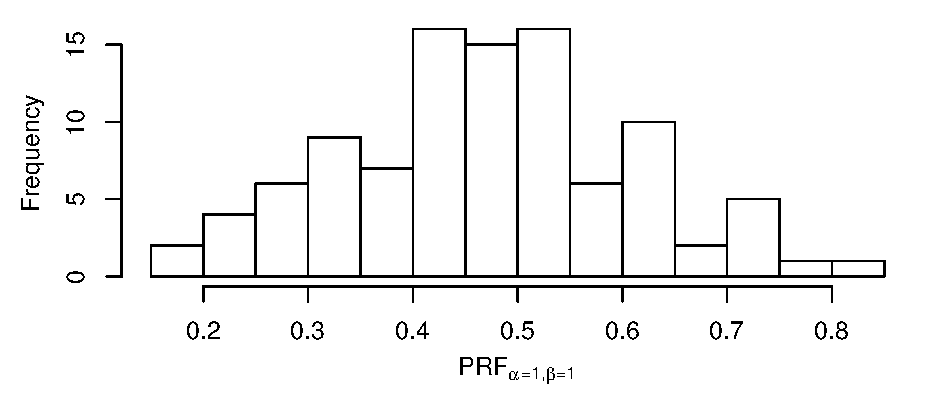
\includegraphics[width=0.8\columnwidth]{figure/qf13-qp-prf.eps}
\end{figure}

\subsection{Selective Query Faceting}
Similar to the idea of selective query expansion~\cite{cronen2004framework,amati2004query,yom2005learning} we can selectively present facets to users based on the query facet extraction performance of each query. Ideally, we only show facets for good performing queries and avoid bad ones to improve user satisfaction: in the precision-oriented scenario, it may be more desirable to leave users with a clean keyword-search interface than to show poor-quality facets. To support this selective query faceting, a key problem is the prediction of the query facet extraction performance. We find a simple score based on the expectation of \PRF can predict extraction performance fairly well.

\subsection{Performance Prediction}
In performance prediction, our goal is to predict the extraction performance for a given query with its extracted facets. We focus on predicting \PRF, and leave prediction of other measures as future work. The prediction could be done by using single indicator scores (like the clarity score in prediction retrieval performance~\cite{cronen2002predicting}), or by combining different features using regression or classification models. No matter which approach, we first need to find good indicators/features for estimating the performance. 

To find effective features, a natural way is to investigate the probabilistic model we have already learned in the QF method, because the learned probabilities already incorporate beliefs about the correctness of corresponding outputs. For example, we can use the term probability $P(y_i|t_i)$ defined in Equation~\ref{eq:y} to estimates the chance that the output terms are indeed facet terms, and use the pairs probability $P(z_{i,j}|p_{i,j},y_i,y_j)$ defined in Equation~\ref{eq:z} to estimate the chance that the term pairs in the same extracted facets indeed belong to a query facet. 

In order to use the term and pair probabilities as features, we need to aggregate them in some ways, because these probabilities are for terms and pairs, not directly for whole extracted facet set. We investigates two ways of aggregation. First, from the perspective of data fitness, we can directly use log-likelihood of extracted facets to measure the fitness. For example, we can use the whole log-likelihood based on Equation~\ref{eq:ll}, and we can also use the log-likelihood for only the terms or only the pairs based on the first term and second terms in the equation respectively. 

Second, from the perspective of directly estimating utility (performance), we can aggregate the probabilities for estimating \PRF directly in a similar way as our empirical utility maximization approach. More specially, we can estimate \PRF performance based on the expected term and pair quantities under the learned model. The estimates can be obtained as follows,
\begin{equation}
\label{eq:mest} % measure estimates
\begin{split}
\widehat{T\!P}=\frac{\sum_i P(t_i)y_i}{\sum_i y_i}, &\;\; \widehat{T\!R}=\frac{\sum_i P(t_i)y_i}{\sum_i P(t_i)},\\ 
\widehat{P\!T}=\frac{\sum_{i,j} P(p_{i,j})z_{i,j}}{\sum_{i,j} z_{i,j}},&\;\; \widehat{P\!R}=\frac{\sum_{i,j} P(p_{i,j})z_{i,j}}{\sum_{i,j} P(p_{i,j})y_iy_j},
\end{split}
\end{equation}
where we use $P(t_i)\equiv P(y_i\!=\!1|t_i)$, $P(p_{i,j})\equiv P(z_{i,j}\!=\!1|p_{i,j}, y_i\!=\!1,y_j\!=\!1)$ for simplification. Estimates of \TF, \PF and can be easily obtained by substituting \TP, \TR, \PP, \PR with their estimates in the corresponding equations in Section~\ref{sec:precision-measure}. Estimate of \PRF can be obtained by substituting \TP, \TR and \PF with their estimates in Equation~\ref{eq:prf}. We call this estimate of \PRF the ``PRF score''.

To investigate the effectiveness of the two types of features, we analyze the correlation between extraction performance and each individual feature. We show the correlation results for \QFI's \PRFab{1}{1} performance in Table~\ref{tab:cor}. (\QFI is tested using cross-validation on the \DQF dataset, which will be described in Section~\ref{sec:precision-experiment}, under maximum likelihood estimation training. Observations are similar for other runs.) 

\todo{May be I should call them posteriors}
In the table, the utility-based features \TP, \TR, \PP, \PR, \TF, \PF, $P\!R\!F\!$ (PRF score)  are estimated according to Equation~\ref{eq:mest} as described before. Likelihood-based feature $LL_{sum}=\sum_i{\log P(y_i|t_i)} + \sum_{i,j}{\log P(z_{i,j}|p_{i,j},y_i,y_j)}$ calculates the likelihood of extracted facets based on Equation~\ref{eq:ll}. $tLL_{sum}$ and $pLL_{sum}$ separate log-likelihood that accounts for term and pair in $LL_{sum}$. Average log-likelihoods $tLL_{avg}$, $pLL_{avg}$ are calculated by averaging $tLL_{sum}$ and $pLL_{sum}$ by the number of candidate terms $tSize$ and the number of pairs of selected terms (\ie, $y_i=1$), $pSize$.
\begin{table}[!ht]
\centering
\caption{The correlation of the individual features with \QFI's \PRFab{1}{1} performance. \QFI is tested using cross-validation on \DQF dataset under maximum likelihood estimation training. Feature name abbreviation explanation:  initial ``$t$'' -- ``term'', initial ``$p$'' -- ``pair'', $LL$ -- ``log-likelihood'', $avg$ -- ``average'', ``$std$'' -- ``standard deviation'', $tSize$ -- $|T_\mathcal{L}|$, $pSize$ -- $|P_\mathcal{F}|$.}
\label{tab:cor}
\begin{tabular}{|l|r|l|} \hline
Feature & Correlation & P-value\\ \hline
$P\!R\!F$ & 0.6249 & $3.6\times10^{-12}$\\ \hline
\TF & 0.5933 & $7.7\times10^{11}$\\ \hline
\TR & 0.5817 & $2.2\times10^{-10}$\\ \hline
$tLL_{avg}$ & 0.5709 & $5.5\times10^{-10}$\\ \hline
$tProb_{sum}$ & 0.5527 & $2.4\times10^{-9}$\\ \hline
$tSize$ & 0.5512 & $2.8\times10^{-9}$\\ \hline
\PF & 0.4962 & $1.5\times10^{-7}$\\ \hline
\PR & 0.4878 & $2.6\times10^{-7}$\\ \hline
%pInterProbSum & 0.4598 & $1.4\times10^{-6}$\\ \hline
$pLL_{sum}$ & -0.4513 & $2.4\times10^{-6}$\\ \hline
$pSize$ & 0.4487 & $2.8\times10^{-6}$\\ \hline
$pProb_{sum}$ & 0.4435 & $3.8\times10^{-6}$\\ \hline
%pInterSize & 0.4419 & $4.1\times10^{-6}$\\ \hline
$LL_{sum}$ & -0.4371 & $5.4\times10^{-6}$\\ \hline
\PP & 0.4015 & $3.4\times10^{-5}$\\ \hline
%$pProb_{max}$ & 0.3904 & $5.9\times10^{-5}$\\ \hline
\TP & 0.3336 & $6.9\times10^{-4}$\\ \hline
$pLL_{avg}$ & 0.3329 & $7.1\times10^{-4}$\\ \hline
%pInterProbAvg & -0.3234 & 0.0010\\ \hline
%pInterProbMin & -0.3218 & 0.0011\\ \hline
$pProb_{std}$ & -0.3162 & 0.0014\\ \hline
$tLL_{sum}$ & -0.2317 & 0.0203\\ \hline
$pProb_{min}$ & -0.1984 & 0.0478\\ \hline
$tProb_{min}$ & -0.1391 & 0.1674\\ \hline
%pInterProbMax & 0.1102 & 0.2752\\ \hline
$tProb_{std}$ & -0.1094 & 0.2787\\ \hline
$tProb_{max}$ & 0.03447 & 0.7335\\ \hline
%pInterProbStd & 0.0026 & 0.9793\\ \hline
\end{tabular}
\end{table}

From Table~\ref{tab:cor}, first we find that PRF score has strong correlation (0.6249 with p-value $3.6\times 10^{-12}$) with the performance $P\!R\!F_{\alpha=1,\beta=1}$. This suggests 1) the PRF score is a good indicator for extraction performance, and might be effective in performance prediction, and 2) our estimation of $P\!R\!F_{\alpha=1,\beta=1}$ based on its expectation is effective. Second, we find utility-based features PRF scores, $\widehat{TF}$, $\widehat{TR}$ correlate better with \PRF performance than other likelihood-based features. This validates our assumption that likelihood can be loosely related to the performance measure, and utility could be a better optimization objective.

We combine the proposed features in linear regression and logistic regression models. However, we find the results are not significantly better than simply using PRF score for prediction, which could be caused by the linear dependence between those features. Thus, we propose to use only the  PRF score for query facet extraction performance prediction, which is simple and effective as we will show in Section~\ref{sec:precision-experiment}. We also test other features based on statistical aggregates of the term and pair probabilities, including minimum, maximum, mean, sum and standard deviation. However, they show relatively low correlation with \PRF, and thus we do not report the results here. 

After choosing PRF score as the performance predictor, selective query faceting can be easily done by thresholding this score to decide to show or avoid showing query facet results for each query. We carry out experiments to evaluate its effectiveness in next.


\section{Experiments}
\label{sec:precision-experiment}
Our experiments aim to investigate mainly three research questions. First, we want to test whether existing query facet extraction methods adapt to precision-oriented scenarios. Second, we want to test if our empirical utility maximization approach is effective in precision-oriented scenarios. Last, we want to test whether the PRF score can effectively predict extraction performance, and support selective query faceting. We will first describe our experimental settings, then present experimental results for each of the research questions.

\subsection{Experimental Settings}
\subsubsection{Data}
\todo{name the data set in query face extraction chapter}
We use the same data set as in Chapter~\ref{ch:intrinsiceval}. We call the data set \DQF. \DQF contains 100 web search queries, their top 100 web search results from a commercial web search engine, and their query facet annotation. The query facet annotation was done by pooling facet results from different models, and then having the pooled terms re-grouped by human annotators into query facets. Our candidate lists are extracted as described in Chapter~\ref{ch:facet}.

\subsubsection{Evaluation}
We use \PRF as the evaluation measures, as well as term precision (\ie, \TP), term recall (\ie, \TR), and term clustering F1 (\ie, \PF). 
We choose this measure because it has the flexibility of adjusting emphasis between ``facet precision'' and ``facet recall'', which naturally suits well with the precision-oriented problem.
When $\alpha\!=\!\beta=\!1\!$, \PRFab{1}{1} is used to evaluate the case where term precision, term recall and term clustering are equally important. To evaluate facets under precision-oriented scenarios, we set a high $\alpha \in \{2, 3, \dots, 10\}$ with fixed $\beta\!=\!1$. The settings correspond to the cases where term precision is twice to ten times as important as both term recall and term clustering. Without any prior knowledge, it is more fair to assume that term precision and clustering are equally important (they are both ``precision'' factors for query facets), therefore we will focus more on only down-weighting term recall by setting $\beta \in \{\frac{1}{2}, \frac{1}{3}, ..., \frac{1}{10}\}$ or equivalently $\frac{1}{\beta} \in \{2, 3, \dots, 10\}$ with fixed $\alpha\!=\!1$. These settings correspond to the case where term precision and clustering are twice to ten times as importance as term recall. As before, we evaluate top the 10 facets returned from each model.

We use 10-fold cross validation on \DQF for training, tuning (if applicable) and testing models. Models are tuned on the same \PRF measure that they are tested on. Unless otherwise specified, statistical significance testing is performed by using paired t-test with 0.05 as the p-value threshold.

%\cmt{We will describe how we evaluate for extraction performance prediction and the selective method in Section X}

\subsubsection{Methods}
We study five query facet extraction models briefly summarized as below.
\begin{itemize}
\item \PLSA and \LDA (Section~\ref{sec:facet-other}): pLSA and LDA are applied on candidate facets for facet refining. %The assumption is like documents in the conventional setting, candidate facets are generated by a mixture of hidden topics, which are the query facets in our case. 
After training, the topics are returned as query facets, by using the top terms in each topic. We tune the number of facets and number of facet terms in each facet. The topic model methods in facet refining only uses term co-occurrence information.
\item \QDM (Section~\ref{sec:facet-other}): this is an unsupervised clustering method that applies a variation of the Quality Threshold clustering algorithm~\cite{heyer1999exploring} to cluster the candidate facets with bias towards important ones. 
%Then it ranks/selects the clusters and the terms in those clusters based on TF/IDF-like scores. 
This method incorporates more information than just term co-occurrence, but it is not easy to add new features into the model to further improve the performance.
We tune the diameter threshold, weight threshold for valid cluster and the threshold for selecting terms.
\item \QFI and \QFJ (Section~\ref{sec:facet-infer}): the two models incorporate a rich set of features and learn from labeled data. They were found to be the best across several evaluation measures in Chapter~\ref{ch:intrinsiceval}, therefore we primarily focus on them. Beyond the difference of independent and joint inference, the two models are different in that \QFI has parameters that can be tuned for given measures, while \QFJ does not, as it tries to optimize log-likelihoods. For \QFI, we tune the weight threshold for facet terms $w_{min}$, and the diameter threshold $dia_{max}$.
\end{itemize}

%In the original work, some features are extracted from candidate facets, which are extracted based on different patterns. Since the quality of the extraction patterns may vary, we expand these features by extract them from each individual types of candidate facets. This is more effective according to our experiment (, but due to space limitation, we do not report this result.) 
%supervised methods based on a graphical model, proposed in our previous work~\cite{kong2013extracting}. The graphical model learns how likely it is that a term in the candidate facets should be selected in the query facets, and how likely two terms are to be grouped together into a same query facet, using a rich set of features. Then, based on the likelihood scores, QF-I selects the terms and clusters the selected terms into query facets, while QF-J repeats the procedure, trying to performance joint inference. The two methods were shown to be more effective than the other  methods, because they incorporate more information into the models and learn from available human labels.

We study two ways of training the graphical model (see Section~\ref{sec:facet-gm}) for \QFI and \QFJ.
\begin{itemize}
\item \MLE (Section~\ref{sec:facet-train}): Uses conditional likelihood as the optimization objective and performs maximum likelihood estimating for training.
\item \EUM (Section~\ref{sec:precision-eum}): since likelihood is loosely related to the performance measure, we propose to use empirical utility maximization to directly optimize the \PRF measure during training. We approximate \PRF by its expectation in order to enable numerical optimization. With different $\alpha,\beta$, we can use different versions of \PRF as the optimization objective. We test three runs by setting $(\alpha\!=\!1,\beta\!=\!1)$, $(\alpha\!=\!2,\beta\!=\!1)$, $(\alpha\!=\!1,\beta\!=\!\frac{1}{2})$. 
%\cmt{explain why not others}. 
We denote the different runs by add $\alpha,\beta$ subscript in ``\EUM'' (\eg, \EUMab{2}{1} stands for EUM training using \PRFab{2}{1} as the optimization objective).
\end{itemize}
\subsection{Existing Methods Under Precision-Oriented Scenarios}
\label{sec:precision-existing}
We first investigate if the five existing models can adapt to precision-oriented scenarios by evaluation based on \PRF with different $\alpha,\beta$ settings. In Figure~\ref{fig:existing}, we show \PRF performance of different $\alpha$ (\ie, term precision is more important than term recall and clustering) on the left, and of different $\beta$ (\ie, term precision and clustering are more important than term recall) on the right. We test all the five models with \QFI, \QFJ trained by \MLE. 
%We report results on \DFWS (observations are similar for \DQF).
\begin{figure}[!ht]
\centering
\caption{$P\!R\!F_{\alpha,\beta}$ performance with different $\alpha$ (left, fixed $\beta\!=\!1$) and different $\beta$ (fixed $\alpha\!=\!1$, right) settings for existing methods on \DQF.}
\label{fig:existing}
\begin{subfigure}[b]{0.45\columnwidth}
\includegraphics[width=\columnwidth]{figure/qf13-prfa-5models.eps}
\caption{\DQF, $P\!R\!F_{\alpha,\beta=1}$}
\end{subfigure}
\begin{subfigure}[b]{0.45\columnwidth}
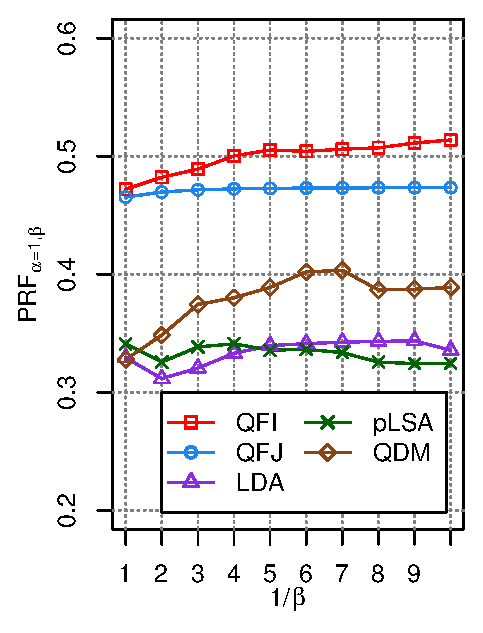
\includegraphics[width=\columnwidth]{figure/qf13-prfaf-5models.eps}
\caption{\DQF, $P\!R\!F_{\alpha=1,\beta}$}
\end{subfigure}
%\begin{subfigure}[b]{0.49\columnwidth}
%\includegraphics[width=\columnwidth]{fws14-prfa-5models}
%\caption{$P\!R\!F_{\alpha,\beta=1}$}
%\end{subfigure}
%\begin{subfigure}[b]{0.49\columnwidth}
%\includegraphics[width=\columnwidth]{fws14-prfaf-5models}
%\caption{$P\!R\!F_{\alpha=1,\beta}$}
%\end{subfigure}
\end{figure}

%First, from Figure~\ref{fig:existing}, we can see pLSA and LDA are generally less effective comparing to other models in both the normal case (\ie, \PRFab{1}{1}) and precision-oriented cases. This suggests topic modeling approach, which only incorporates term co-occurrence information, does not suit the facet extraction problem well, which was also find in the previous work~\cite{kong2013extracting}.
First, we find \QFJ does not adapt well to precision-oriented scenarios. From the figure, we can see the superiority of \QFJ over other models becomes less evident, when moving from the normal case (low $\alpha$ or high $\beta$) to precision-oriented cases (high $\alpha$ or low $\beta$). This because that \QFJ tries to optimize log-likelihood for inferencing, and it cannot be tuned on the performance measures like other models. So it returns the same results for the normal case and precision-oriented scenarios. Second, we generally find that \QFI and \QDM can adapt better than the other models to the precision-oriented scenarios, with \QFI consistently better than all the other models on both datasets. The adaptability of the two models can be explained by their tuning procedure. For example, depending on the target performance measure, \QFI can set different threshold $w_t$ for selecting facet terms. Overall, we find \QFI (under \MLE training) is the best among these existing models for the normal case, as 
well as precision-oriented cases.
 
To further analyze how \QFI adapts to the precision-oriented scenarios, in Table~\ref{tab:qfi}, we report \PRF together with \TP, \TR, \PF and facet size (the total number of terms returned for a query) when setting different $\beta$ in \PRF. 
%For comparison, we also include the results of \QFJ in the last row. Please note \QFJ's \TP, \TR, \PF are all the same for all $\beta$ settings (\ie, no tuning capability), and its \PRF performance is based $\alpha\!=\!1,\beta\!=\!1/10$. 
\begin{table}[!ht]
\centering
\caption{$P\!R\!F_{\alpha,\beta}$ performance with its \TP, \TR, \PF under different $\beta$ settings (fixed $\alpha\!=\!1$) for \QFI on \DQF. ``Size'' reports the average number of terms returned for each queries.}
\label{tab:qfi} 
\begin{tabular}{|r|l|l|l|l|l|} \hline
$\frac{1}{\beta}$ & \PRF & TP & TR & PF & Size\\ \hline
1 & 0.4720 & 0.4450 & 0.4881 & 0.6209 & 89.5\\ \hline
2 & 0.4822 & 0.4896 & 0.4186 & 0.6192 & 70.7\\ \hline
3 & 0.4891 & 0.5108 & 0.3574 & 0.5989 & 56.5\\ \hline
4 & 0.5003 & 0.5291 & 0.3498 & 0.5925 & 53.0\\ \hline
5 & 0.5053 & 0.5348 & 0.3306 & 0.5928 & 48.9\\ \hline
6 & 0.5042 & 0.5343 & 0.3194 & 0.5834 & 47.1\\ \hline
7 & 0.5060 & 0.5343 & 0.3194 & 0.5834 & 47.1\\ \hline
8 & 0.5072 & 0.5343 & 0.3194 & 0.5834 & 47.1\\ \hline
9 & 0.5112 & 0.5364 & 0.3172 & 0.5864 & 46.7\\ \hline
10 & 0.5138 & 0.5365 & 0.3097 & 0.5824 & 45.2\\ \hline
%\hline QFJ & 0.4734 & 0.3986 & 0.4832 & 0.6961 & 97.0\\ \hline
\end{tabular}
\end{table}

From Table~\ref{tab:qfi}, we find that as term recall factor becomes less and less important (or equivalently as the precision factors becomes more and more important), \QFI becomes more and more conservative in selecting terms. The number of terms returned on average for each query (``size'' in the table) decreases from 89.5 to 45.2. Term precision \TP thus increases significantly, while term recall \TR and term clustering \PF decrease. This indicates, by tuning on the performance measure, \QFI tries to find a good balance between the tree factors for each scenarios. 

\subsection{Empirical Utility Maximization Performance}
Next, we compare \EUM  and \MLE training to test the effectiveness of the EUM approach we proposed. We first compare \EUM and \MLE training using both \QFI and \QFJ in Figure~\ref{fig:ll-prf}. We report results for $P\!R\!F_{\alpha=1,\beta}$ (\ie, fixed $\alpha=1$ with different $\beta$ settings) on \DQF. Observations are similar for other cases. The figure shows \QFI with \EUM and \MLE training on the left, and \QFJ results on the right. We report three runs of \EUM, which use \PRF under different $\alpha,\beta$  settings (specified in the legend) as the training target.


\begin{figure}[!ht]
\centering
\caption{$P\!R\!F_{\alpha=1,\beta}$ performance for \MLE and \EUM training using \QFI (left) and \QFJ (right) on \DQF. The three \EUM runs use \PRF under different $\alpha,\beta$ settings (specified in the legend) as the training target.}
\label{fig:ll-prf}
\begin{subfigure}[b]{0.45\columnwidth}
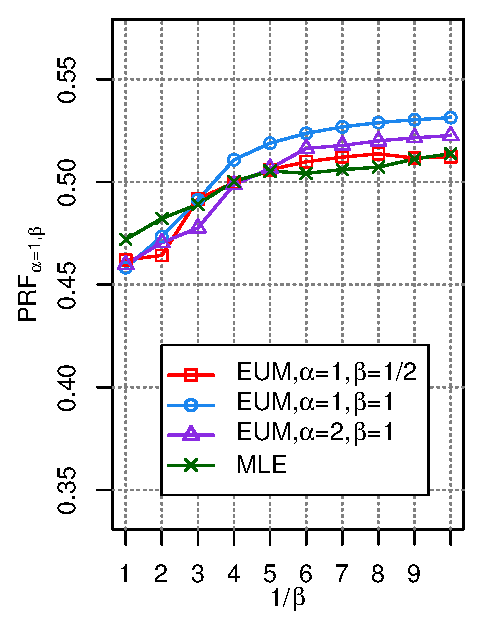
\includegraphics[width=\columnwidth]{figure/qf13-qfi-prfaf-ll-prf.eps}
\caption{\QFI}
\end{subfigure}
\begin{subfigure}[b]{0.45\columnwidth}
\includegraphics[width=\columnwidth]{figure/qf13-qfj-prfaf-ll-prf.eps}
\caption{\QFJ}
\end{subfigure}
%\begin{subfigure}[b]{0.49\columnwidth}
%\includegraphics[width=\columnwidth]{figure/fws14-qfi-prfaf-ll-prf.eps}
%\caption{\DFWS, \QFI}
%\end{subfigure}
%\begin{subfigure}[b]{0.49\columnwidth}
%\includegraphics[width=\columnwidth]{figure/fws14-qfj-prfaf-ll-prf.eps}
%\caption{\DFWS, \QFJ}
%\end{subfigure}
\end{figure}

From Figure~\ref{fig:ll-prf}, for \QFI, we find there are no statistically significant differences between \MLE and \EUM in most cases, even though generally \EUM obtains slightly better \PRF than \MLE. This can be explained by noting that \QFI under \MLE has already incorporated the \PRF learning target because it is tuned on \PRF. Essentially, we can view \QFI (under \MLE training) as a model that is trained on likelihood to find a small tuning space to enable optimization on given performance measures by hand tuning.

Differently, for \QFJ, we find \EUM can improve largely over \MLE under the precision-oriented scenarios. The differences between \EUM and \MLE are statistically significant for all $1/\beta>2$ and for all the three \EUM runs. This indicates 1) utility (performance measure) is a better optimization objective than likelihood and 2) our approximation of \PRF based on its expectation is effective. 


To study how \EUM training affects \QFJ in more details, as an example, we show \PRFab{1}{0.1} together with its \TP, \TR, \PF and facet size in Table~\ref{tab:prf}.
\begin{table}[!ht]
\centering
\caption{\PRFab{1}{0.1} with \TP, \TR, \PF for \MLE and \EUM training on \DQF. Subscripts of \EUM indicates the $\alpha,\beta$ setting used for its optimization target \PRF. }
\label{tab:prf}
\begin{tabular}{|l|l|l|l|l|l|l|} \hline
model & Training & \PRF & TP & TR & PF & Size\\ \hline
%\QFI & \MLE & 0.5138 & 0.5365 & 0.3097 & 0.5824 & 45.2\\ \hline
%\QFI & \EUMab{1}{1} & 0.5123 & 0.5250 & 0.2999 & 0.6021 & 45.7\\ \hline
%\QFI & \EUMab{2}{1} & 0.5226 & 0.5455 & 0.2588 & 0.6073 & 37.8\\ \hline
%\QFI & \EUMab{1}{0.5} & 0.5313 & 0.5426 & 0.2724 & 0.6180 & 41.0\\ \hline\hline
\QFJ & \MLE & 0.4734 & 0.3986 & 0.4832 & 0.6961 & 97.0\\ \hline
\QFJ & \EUMab{1}{1} & 0.5223 & 0.4884 & 0.3341 & 0.6702 & 54.8\\ \hline
\QFJ & \EUMab{2}{1} & 0.5696 & 0.5711 & 0.2328 & 0.6705 & 33.9\\ \hline
\QFJ & \EUMab{1}{0.5} & 0.5607 & 0.5710 & 0.2229 & 0.6620 & 33.0\\ \hline
\end{tabular}
\end{table}

From Table~\ref{tab:prf}, first, we can see when trained on \EUM under precision-oriented settings (\ie,\EUMab{2}{1} and \EUMab{1}{0.5}), \QFJ are more conservative in selecting terms than in \MLE training. When moving from \MLE to \EUM training, its facet size becomes much smaller (\ie, 97 to 33), \TP increases greatly while \TR decreases substantially. This effect is desirable under the precision-oriented scenarios, in which we care much more about precision than recall, as reflected by the improvement in \PRFab{1}{0.1} shown in the table.

Second, by comparing \EUMab{1}{1} with \EUMab{2}{1}, \EUMab{1}{0.5} in Table~\ref{tab:prf}, we can see \EUMab{2}{1}, \EUMab{1}{0.5} trained models behave more conservatively than \EUMab{1}{1} trained models. This suggest our training is effective -- as we change the training target \PRF parameter from $(\alpha=1,\beta=1)$ to $(\alpha=2,\beta=1)$ and $(\alpha=1,\beta=0.5)$), it learns that we are putting more emphasis on precision, and thus behaves more conservatively.

Last, the improvement of \QFJ in precision oriented scenarios raises a question -- will it outperform the previous best model, \QFI, under precision-oriented scenarios? We test this in Figure~\ref{fig:qfi-qfj}. In the figure, we compare \QFJ under \EUM training with other baselines, including \QFI under \MLE (representing the state-of-the-art baseline) and \EUM training. We report results under \EUMab{1}{0.5} training on \DQF (results are similar in other cases). From the figure we find \QFJ under \EUM training outperforms other models in the precision-oriented scenarios. The difference between \QFJ,\EUM and the state-of-the-art method \QFI,\MLE are statistically significant for $P\!R\!F_{\alpha=1,\beta}$ when $\frac{1}{\beta}>4$.
\begin{figure}[!ht]
\centering
\caption{\PRF performance with different $\alpha$, $\beta$ settings for \QFI and \QFJ under \MLE and \EUM training on \DQF. \EUMab{1}{0.5} run result is reported for \EUM.}
\label{fig:qfi-qfj}
\begin{subfigure}[b]{0.45\columnwidth}
\includegraphics[width=\columnwidth]{figure/qf13-prfa-qfi-qfj.eps}
\caption{$P\!R\!F_{\alpha,\beta=1}$}
\end{subfigure}
\begin{subfigure}[b]{0.45\columnwidth}
\includegraphics[width=\columnwidth]{figure/qf13-prfaf-qfi-qfj.eps}
\caption{$P\!R\!F_{\alpha=1,\beta}$}
\end{subfigure}
%\begin{subfigure}[b]{0.49\columnwidth}
%\includegraphics[width=\columnwidth]{fws14-prfa-qfi-qfj}
%\caption{\DFWS, $P\!R\!F_{\alpha,\beta=1}$}
%\end{subfigure}
%\begin{subfigure}[b]{0.49\columnwidth}
%\includegraphics[width=\columnwidth]{fws14-prfaf-qfi-qfj}
%\caption{Fws14, $P\!R\!F_{\alpha,\beta=1}$}
%\end{subfigure}
\end{figure}

\subsection{Extraction Performance Prediction}
To predict query facet extraction performance, we build linear regression models using only the PRF score (see Section~\ref{sec:precision-selective}) as the feature (with intercept). We test the models for predicting \PRF under different $\alpha,\beta$, based on 10-fold cross validation on \DQF for \QFI in Table~\ref{tab:regression}. We report root-mean-square deviation (RMSD), Pearson correlation (R), and p-values for the significance of correlation. %(observations are similar for \QFJ runs). 
\begin{table}[!ht]
\centering
\caption{Linear regression results based on 10-fold cross-validation for predicting \PRF performance. RMSD -- root-mean-square deviation, R -- Pearson correlation.}
\label{tab:regression}
\begin{tabular}{|l|l|l|l|} \hline
Measure & RMSD & R & p-value\\ \hline
\PRFab{1}{1} & 0.1110 & 0.6112 & $1.4\times10^{-11}$\\ \hline
\PRFab{1}{0.2} & 0.1800 & 0.5745 & $4.1\times 10^{-10}$\\ \hline
\PRFab{1}{0.1} & 0.1882 & 0.5566 & $1.8\times 10^{-9}$\\ \hline
\PRFab{5}{1} & 0.2109 & 0.2958 & 0.0028\\ \hline
\PRFab{10}{1} & 0.2245 & 0.4028 & $3.2\times 10^{-5}$\\ \hline
%\hline
%\QFJ & \PRFab{1}{1} & 0.1177 & 0.5916 & $9.1\times 10^{-11}$\\ \hline
%\QFJ & \PRFab{1}{0.2} & 0.2073 & 0.4717 & $7.2\times 10^{-7}$\\ \hline
%\QFJ & \PRFab{1}{0.1} & 0.2239 & 0.4164 & $1.6\times 10^{-5}$\\ \hline
%\QFJ & \PRFab{5}{1} & 0.2057 & 0.4189 & $1.4\times 10^{-5}$\\ \hline
%\QFJ & \PRFab{10}{1} & 0.2360 & 0.3182 & 0.0013\\ \hline
\end{tabular}
\end{table}

The results in Table~\ref{tab:regression} show fairly strong RMSD values and strong positive correlations between the predicted \PRF and real \PRF performance for most cases. For example, p-value $1.4\times10^{-11}$ for the first row indicates that it is extremely unlikely that the predicted \PRFab{1}{1} performance has no relationship with the actual performance. We also see one exception. For \PRFab{5}{1} we only see fair correlation, which may be because that we use $\alpha\!=\!1,\beta\!=\!1$ for computing our PRF score, while in \PRFab{5}{1} the three factors are more unbalanced weighted.

\subsection{Evaluating Selective Query Faceting}
Next, we study the effectiveness of selective query faceting based on the predicted score (from cross validation). Recall that our selective method is done by thresholding the predicted performance for deciding whether to show or avoid showing facets for each query (see Section~\ref{sec:precision-selective}). There is a trade-off between the performance of selected queries and the coverage of queries for query faceting. With a higher threshold, selective query faceting would select fewer queries to show facets, but users should obtain better performance for the facets that are presented to them. On the contrary, a lower threshold will result in selecting more queries to show facets, but the performance for the selected queries may be worse. 

To evaluate selective query faceting, we plot the average \PRF performance for queries selected by PRF score, when using different thresholds in Figure~\ref{fig:selective}. The x-axis indicates the number of selected queries, while the y-axis indicates the average \PRF performance for those selected queries. In addition to average \PRF, we also plot the standard error with 95\% confidence intervals by the gray area (except for the case where only one query is selected). We report results on \DQF for a \QFI run that are trained under \MLE and evaluated on \PRFab{1}{1}. 
%(Observations for other runs are similar.) 
%The two runs represent the best model for normal cases and precisely-oriented scenarios respectively.
\todo{Need to stress that the number of queries changes. So the comparison may make no sense}

\begin{figure}[!ht]
\centering
\caption{Average \PRF performance for selected queries. The gray area indicates standard error with 95\% confidence intervals. Run: \PRFab{1}{1} as the measure with \MLE trained \QFI as the extraction model}
\label{fig:selective}
\includegraphics[width=0.8\columnwidth]{figure/qf13-qp-prf-ll.eps}
%\begin{subfigure}[b]{1\columnwidth}
%\includegraphics[width=0.8\columnwidth]{qf13-qp-prf-ll}
%\end{subfigure}
%\begin{subfigure}[b]{1\columnwidth}
%\includegraphics[width=\columnwidth]{qf13-qp-prfb01-prfb05}
%\caption{Run: \PRFab{1}{0.1} as measure with \EUMab{1}{0.5} trained \QFJ extraction model.}
%\end{subfigure}
\end{figure}

From Figure~\ref{fig:selective}, we can see as we select fewer and fewer queries for presenting facets, generally the average performance for the selected queries increases. This indicates the query faceting method is fairly effective in selecting good performing queries and avoiding bad ones. When 20 queries are selected, we obtain 0.5792 \PRFab{1}{1} for the selected queries, comparing to 0.4720 when the selective method is not performed (\ie, showing facets for all queries). The difference are statistically significant according to two-tailed two-sample t-test (p-value = 0.0034). 

%The observation for Figure~\ref{fig:selective}(b) is similar but less evident. We also find statistical significant improvement when applying selective faceting. For example, when selecting 20 queries, we obtain 0.6986 \PRFab{1}{0.1}, comparing to 0.5607 when the selective method are not performed (p-value = 0.0011).

\section{Summary}
\label{sec:precision-conclusion}
In this chapter, we studied and improved query facet extraction under precision-oriented scenarios, which could help this technique to be used practically. We find the performance expectation can be used as an approximation to directly optimize the performance measure, which significantly improves existing models under precision-oriented scenarios. We proposed a PRF score based on the expectation of \PRF to predict extraction performance. We show this score has fairly good prediction performance which enables selective query faceting that selects good performing queries to show facets, and improves the average extraction performance.

In next chapter, we will consider how to re-organize search results based on users' selection on the extracted query facets.
\chapter{Facet Feedback}
\label{ch:feedback}
\section{Introduction}
\label{sec:fdbk-intro}
\textbf{Facet feedback}~\cite{kong2014extending} is to adjust (filter or re-rank) the search results based on users' selections on the provided facets (corresponding to step 5 in Figure~\ref{fig:fws-example}). Boolean filtering, which filters search results by requiring selected terms to appear, is the dominant facet feedback method used in conventional faceted search. However, it may be too strict when extended to the open-domain setting. Boolean filtering is based on two assumptions~\cite{zhang2010interactive}: (1) users are clear about what they are looking for, and thus are able to select proper terms to restrict the results; and (2) matching between a term and a document is accurate and complete. In FWS, that means a document that contains the selected term should be relevant to the term, and all documents relevant to that selected term should contain the term. Neither of the two assumptions are likely to hold in FWS.
Therefore, we propose soft ranking models that expand original queries with user selected terms for re-ranking.

In this chapter we describe the two types of models we explore for facet feedback: Boolean filtering and soft ranking. We will first define notations used in facet feedback models in Section~\ref{sec:fdbk-notations}, and then present Boolean filtering and soft ranking models in Section~\ref{sec:fdbk-filter} and Section~\ref{sec:fdbk-ranking} respectively.  We will explore the effectiveness of these approaches in Chapter~\ref{ch:extrinsiceval}. 
%The work in this chapter is completed and published~\cite{kong2014extending}.

\section{Related Work}
\label{sec:feedback-related}
There is a long history of using user explicit feedback to improve retrieval performance. In relevance feedback~\cite{rocchio71relevance,salton1997improving}, documents are presented to users for judgment, after which terms are extracted from the judged relevant document, and added into the retrieval model. In the case where true relevance judgment is unavailable, top documents are assumed to be relevant, which is called pseudo relevance feedback~\cite{buckley1995automatic,abdul2004umass}. Because document is a large text unit, which can be difficult for users to judge and for the system to incorporate relevance information, previous work also studied user feedback on passages~\cite{allan1995relevance,xu1996query} and terms~\cite{koenemann1996case,tan2007term}. For faceted search, \citet{zhang2010interactive} study user feedback on facets, using both boolean filtering and soft ranking models. However, the study is based on corpora with human created facet metadata, which is difficult to 
obtain for the  general web.  One other difference between our work and most other user feedback work is that facet feedback in our work is used to improve ranking with respect to the query subtopic specified by the feedback terms, instead of the query topic represented by the original query. This presents the scenario in FWS, where users start with a less-specified query, and then use facets to help clarify and search for subtopic information.

\section{Notations} \label{sec:fdbk-notations}
We use $t^u$ to denote a \textbf{feedback term} selected by a user $u$, $F^u=\{t^u\}$ to denote a facet that contains feedback terms (a \textbf{feedback facet}), and $\mathcal{F}^u=\{F^u\}$ to denote the set of feedback facets. Given those, a feedback model can be formally denoted as $S'(D,Q,\mathcal{F}^u)$, which gives a score for document $D$ according to the original query $Q$ and the user's feedback $\mathcal{F}^u$. 

\section{Boolean Filtering Model} \label{sec:fdbk-filter}
The Boolean model filters documents based on Boolean operations using the feedback $\mathcal{F}^u$. Similar to \citet{zhang2010interactive}, we study three different Boolean conditions for filtering. We use the AND condition to require that the document contains \emph{all} of the feedback terms in $\mathcal{F}^u$. The AND condition might be too strict, so a relaxed alternative is to use the OR condition, which requires that the document contains \emph{at least one} of the feedback terms. The last Boolean condition, A+O, is somewhere in between the two conditions above. It use AND across different feedback facets in $\mathcal{F}^u$, and OR for terms $t^u$ inside each facet $F^u$. The Boolean feedback model scores a document by
\begin{equation}
S_{B}'(D,Q,\mathcal{F}^u) = \left\{ \begin{array}{ll}
S(D,Q) &\mbox{ if $D$ satisfies condition $B(\mathcal{F}^u)$} \\
-\infty &\mbox{ otherwise}
\end{array} \right.
\end{equation}
where condition $B$ can be either AND, OR, or A+O, and $S(D,Q)$ is the score returned by the original retrieval model. Notice that when there is only a single feedback term, the three conditions will be equivalent; when there is only one feedback query facet (group of feedback terms), OR and A+O will be equivalent.

\section{Soft Ranking Model} \label{sec:fdbk-ranking}
While Boolean filter models are commonly used in faceted search, it may be too strict for FWS, as explained in Section~\ref{sec:fdbk-intro}. %The Boolean filtering model is based on two assumptions~\cite{zhang2010interactive}: (1) users are clear about what they are looking for, and thus are able to select proper feedback terms to restrict the results; and (2) matching between a facet term and a document is accurate and complete. In FWS, that means a document that contains the feedback term should be relevant to the term, and all documents relevant to that feedback term should contain the term. However, both of the two assumptions are unlikely to hold in FWS.
Therefore, we also use soft ranking models, which expand the original query with feedback terms, using a linear combination as follows
\begin{equation}
 S_E'(D,Q,\mathcal{F}^u) = \lambda S(D,Q) + (1-\lambda) S_E(D,\mathcal{F}^u)
\end{equation}
where $S(D,Q)$ is the score from the original retrieval model as before, and $S_E(D,\mathcal{F}^u)$ is the expansion part which captures the relevance between the document $D$ and feedback facet $\mathcal{F}^u$, using expansion model $E$. $\lambda$ is a parameter for adjusting the weight between the two parts.

We use two expansion models, a term and a facet expansion model. The term expansion model, $ST$, assigns equal weight for all the feedback terms, as follow,
\begin{equation}
S_{ST}(D,\mathcal{F}^u) = \frac{1}{N}\sum_{F^u\in\mathcal{F}^u}{\sum_{t^u\in F^u}{S(D,t^u)}}
\end{equation}
where $N$ is the total number of facet terms. $S(D,t^u)$ can be the original retrieval model used for the query or a different model.

The facet expansion model, $SF$, uses the facet structure information. It assigns equal weights between each feedback facets, and equal weights between feedback terms within the same facet, as shown below.
\begin{equation}
S_{SF}(D,\mathcal{F}^u) = \frac{1}{|\mathcal{F}^u|} \sum_{F^u \in \mathcal{F}^u}{ \frac{1}{|F^u|} \sum_{t^u \in F^u}{S(D, t^u)}}
\end{equation}

Notice that the two expansion models will be equivalent when there is only a single feedback term or when there is only one feedback facet. In our experiments, we use the Sequential Dependence Model (SDM)~\cite{metzler2005markov} as the baseline retrieval model $S(D,Q)$, which incorporates word unigrams, adjacent word bigrams, and adjacent word proximity. For $S(D,t^u)$, we use the Query Likelihood model with Dirichlet smoothing as below,
\begin{equation}
S(D,t^u)=\sum_{w\in t^u}{\log\frac{tf(w,D)+\mu\frac{tf(w,\mathcal{C})}{|\mathcal{C}|}}{|D|+\mu}}
\end{equation}
where $w$ is a word in $t^u$, $tf(w,D)$ and $tf(w,\mathcal{C})$ are the number of occurrences of $w$ in the document and the collection respectively; $\mu$ is the Dirichlet smoothing parameter; $|D|$ is the number of word in $|D|$, and $|\mathcal{C}|$ is the total number of words in the collection.

\section{Summary}
In this chapter, we described three Boolean filtering models (AND, OR, A+O) and proposed two soft ranking models (ST and SF) for facet feedback. In the next chapter, we will develop an extrinsic evaluation method for evaluating these feedback models.
\chapter{Extrinsic Evaluation}\label{ch:extrinsiceval}
\section{Introduction}
\label{sec:extrinsic}
The intrinsic evaluation proposed in Chapter~\ref{ch:intrinsiceval} is not based on any particular search task, and thus may not reflect the real utility of the generated facets in assisting search. Therefore, we describe an extrinsic evaluation method which evaluates a system based on an interactive search task that incorporates Faceted Web Search (FWS). We believe the task is similar to a real application of FWS as illustrated in Figure~\ref{fig:fws-example}: a user searches using an under-specified query, the FWS system provides query facets from which the user can select feedback terms that would help further specify the query, after which the FWS system uses the feedback terms for re-ranking documents.

For the extrinsic evaluation, ideally we could ask real users or carry out user studies to try each FWS systems, and measure the gain and cost for using them. The gain can be measured by the improvement of the re-ranked results using standard IR metrics like MAP or nDCG. The cost can be measured by the time spent by the users giving facet feedback. However this evaluation is difficult and expensive to extend for evaluating new systems rapidly.

We instead propose to \emph{simulate} the user feedback process based on a user interaction model, using oracle feedback terms and facet terms collected from annotators. Both the oracle feedback and annotator feedback incrementally select all feedback terms that a user may select, which will then be used in simulation based on the user model to determine which subset of the oracle or annotator feedback terms are selected by a user and how much time is spent giving that feedback. Finally, the systems are evaluated by the re-ranking performance together with the estimated time cost.

For the simulated FWS task, we use the TREC Web track dataset of the diversification task~\cite{clarke2009overview,clarke2010overview,clarke2011overview,clarke2012overview}. It includes query topics that are structured as a representative set of subtopics, each related to a different user need, with relevance judgment made at the subtopic level. In our task, each subtopic is regarded as the search intent of a user, and the corresponding topic title is used as the under-specified query issued to the FWS system. For example, for query number 10 in the TREC 2009 Web Track, the title ``cheap internet'' is used as the initial query, and its subtopic ``I want to find cheap DSL providers'' is regarded as the search intent of the user.

We conduct extrinsic evaluations on combinations of different query facet generation models and facet feedback models in our experiments. We show that by using facet feedback from users, Faceted Web Search is able to assist the search task and significantly improve ranking performance.
Comparing intrinsic evaluation and extrinsic evaluation on different facet generation models, we find that the intrinsic evaluation does not always reflect system utility in real application. Comparing different facet feedback models, we find that the Boolean filtering models, which are widely used in conventional faceted search, are too strict in Faceted Web Search, and less effective than soft ranking models.

In the rest of this Chapter, we first describe how we collect simulated facet feedback in Section~\ref{sec:oa-feedback}. Then, we describe our user model for estimating the feedback time cost to users in Section~\ref{sec:user-model}. Last, we present our experiments for conducting extrinsic evaluation on different faceted web search systems (different combinations of query facet generation models and facet feedback models) in Section~\ref{sec:ee-exp}, followed by conclusions in Section~\ref{sec:ee-conclusions}. 

%The work in this chapter is completed and published~\cite{kong2014extending}.

\section{Oracle and Annotator Feedback} \label{sec:oa-feedback}
Oracle feedback presents an idealized case of facet feedback, in which only \emph{effective} terms -- those that improve the quality of the ranked list -- are selected as feedback terms. We extract oracle feedback terms by testing each single term in the presented facets. Each single candidate term is used by a facet feedback model to re-rank the documents and the candidate term is selected for the oracle if the improvement of the re-ranked documents meets a threshold. In our experiment, we use MAP as the metric and set the threshold to be 0.01. Since we have two types of feedback models, there are two sets of oracle feedback terms --  one uses the Boolean filter models, and one uses the soft ranking models.
%Note that when using a single feedback term, the different feedback models of the same type will have same results, as discussed in Section~\ref{sec:feedback}.

Oracle feedback is cheap to obtain for any facet system (assuming document relevance judgments are available), however it may be quite different from what actual users may select in a real interaction. Therefore, we also collect feedback terms from annotators. Our annotation interface is shown in Figure~\ref{fig:feedback-annotation}. The facet feedback annotation is done by presenting the facets (corresponding to list 1 to 5 in Figure~\ref{fig:feedback-annotation}) to an annotator with description of the information need (corresponding to subtopic description in Figure~\ref{fig:feedback-annotation}) and the initial under-specified query. The annotator is asked to select all the terms from the facets that would help address the information need (corresponding to step 2 in Figure~\ref{fig:feedback-annotation}). Ideally, we could present all the facets generated from different FWS systems for this annotation, but it would be quite expensive. In our experiment, we only present the annotator with facets collected 
from the intrinsic evaluation. This assumes all other facet terms generated by systems are uninteresting to the user or at least not easy for the user to select.

\begin{figure}[H]
\centering
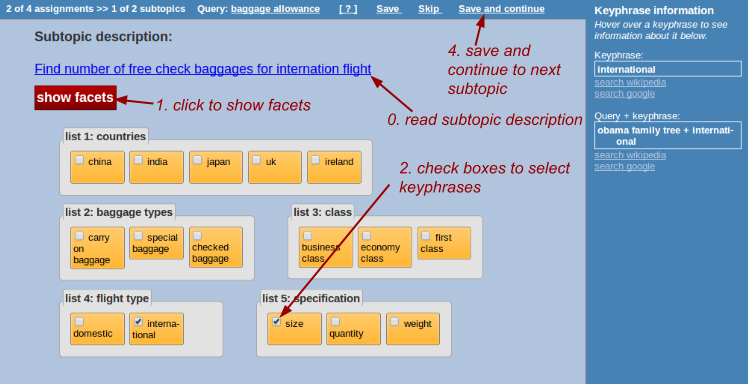
\epsfig{file=figure/feedback-annotation-ui.png,scale=0.55}
%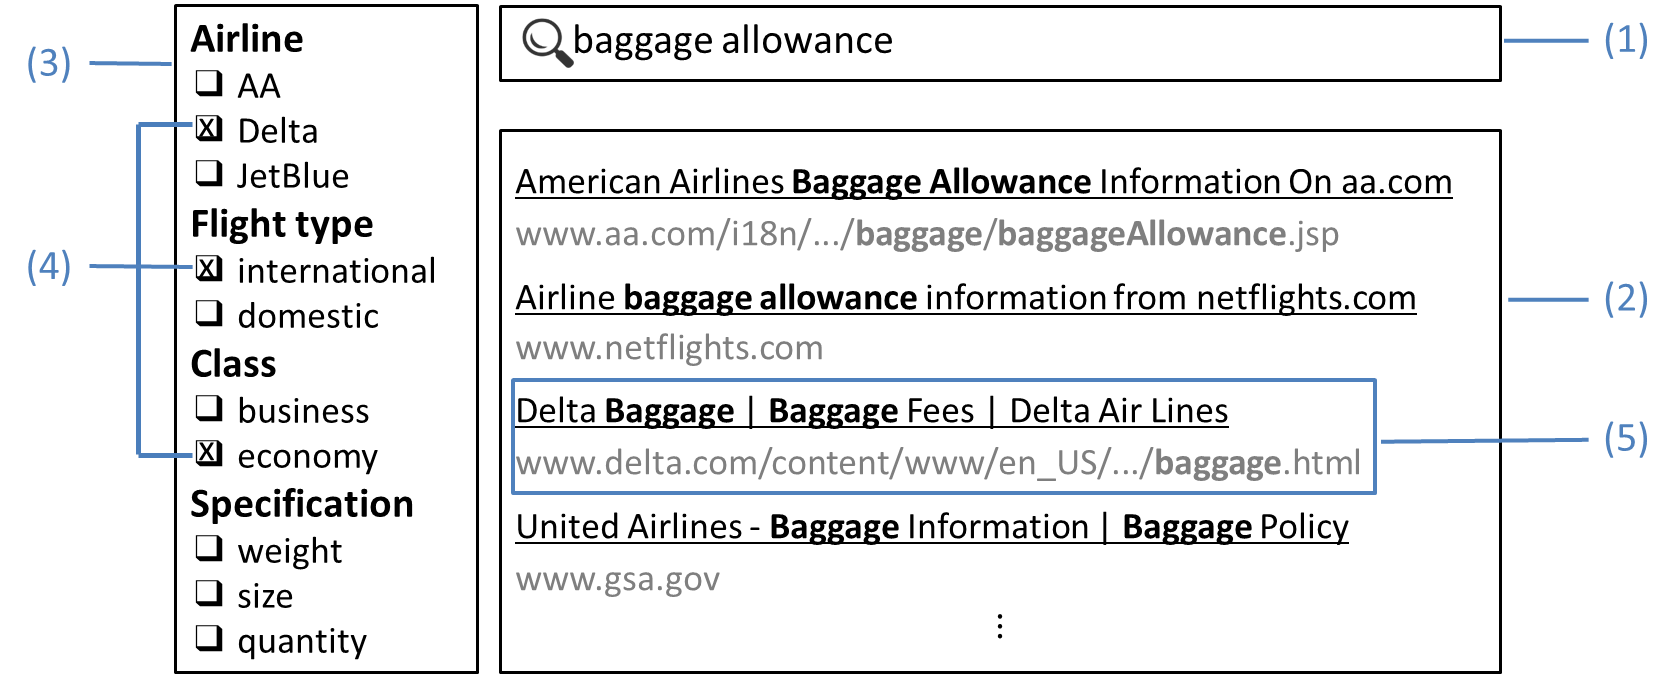
\includegraphics[scale=0.45]{figure/fws-example.png}
\caption{Annotation interface for facet feedback annotation.}
\label{fig:feedback-annotation}
\end{figure}

\section{User Model} \label{sec:user-model}
The user model describes how a user selects feedback terms from facets, based on which we can estimate the time cost for the user. While any reasonable user model can be brought to play here, we use a simple one, similar to the user model others have used for selecting suggestions from clusters of query auto-completions~\cite{jain2010organizing}.

Our user model is based on the structural property of facets. By grouping terms into facets, the facet interface essentially provides a skip list of these facet terms for users. More specifically, in the model, a user sequentially scans presented query facets and skips an entire facet if the user finds the facet irrelevant. Otherwise, the user will scan within the facet, sequentially reading and selecting desired facet terms, until the user finds the desired one or ones. Based on this user model, the time cost for giving facet feedback can be calculated as as,
\begin{equation}
 T(\mathcal{F}^u) = 
\sum_{F^u \in \mathcal{F}^u}{\left( T_f(F^u) + \sum_{t\in ts(F^u)}{T_t(t)} \right)} 
\end{equation}
The righthand side of the equation contains two parts. The first part $T_f(F^u)$ is the time for scanning a facet and deciding relevance, and the second part is the time for scanning/selecting terms in the relevant facets. $ts(F^u)$ is the set of terms scanned/selected in $F^u$'s corresponding query facet, and $T_t(t)$ is the time used for scanning/selecting a term. Since we assume users sequentially scan the terms inside a facet, $ts(F^u)$ will include all the beginning terms in $F^u$'s corresponding facet until the last selected term. This is based on the assumption that users are clear about what terms to select, and stop scanning after finding all of them.
\todo{need to correct the formula}

To simplify the estimation, we further assume time costs are equal for scanning different facets, and equal for scanning/selecting different terms. Then the estimation becomes
\begin{equation}
 T(\mathcal{F}^u) = |\mathcal{F}^u|\cdot T_f + |ts(\mathcal{F}^u)|\cdot T_t
\end{equation}
where $|ts(\mathcal{F}^u)|=\sum_{F^u \in \mathcal{F}^u}{|ts(F^u)|}$ is the total number of term scanned/selected. $T_f$ and $T_t$ are now parameters representing the time for scanning a facet and time for scanning/selecting a term respectively.

To estimate parameters $T_f$ and $T_t$, we tracked annotator behavior during the feedback annotation described in Section~\ref{sec:oa-feedback}, including selecting / un-selecting terms and starting / exiting an annotation session. We only used annotation sessions which did not contain any un-selecting actions, and filtered out some inappropriate sessions, e.g. the annotator dwells for a long time with no activity. This selection results in 274 annotator sessions. We then extracted $|\mathcal{F}^u|$ and $|ts(\mathcal{F}^u)|$ as well as the time cost $T(\mathcal{F}^u)$ for each session, and used linear regression to fit the model to the data. When using sessions from all annotators, $T_f$ and $T_t$ are estimated as 2.60 and 1.60 seconds respectively, with $R^2=0.089$. The low $R^2$ is partly due to the variance introduced by using sessions of different annotators. When using one single annotator we obtain a better fit with $R^2=0.555$, and $T_f=1.51$, $T_t=0.66$, for one of the annotators. Since the 
estimation for $T_f$ is about twice of $T_t$, for simplicity, in our experiment, we set $T_f=2\cdot T_t$, and report the time cost in the time unit of reading/scanning a single term.
\todo{Test $T_f=2\cdot T_t$}

Based on this user model, given oracle/annotator feedback, which represents all the terms that a user may select, the extrinsic evaluation works as follows. We incrementally include each term in oracle/annotator feedback as a feedback terms, and measure how ranking performance changes together with the time cost estimated based on the user model. 

\section{Experiments} \label{sec:ee-exp}
\todo{add an interactive model baseline}
\todo{Call QFI, QFJ consistently}
%In this section, we describes the experiment results for comparing 
\subsection{Experiment Settings}
\textbf{Data set}. For the document corpus, we use the ClueWeb09 Category-B collection and apply spam filtering with a threshold of 60 using the Waterloo spam scores~\cite{cormack2011efficient}. The spam-filtered collection is stemmed using the Krovetz stemmer~\cite{krovetz1993viewing}. For the query topics and subtopics, we used those from TREC Web Track's diversity task from 2009 to 2012, which also contain relevance judgments for documents with respect to each subtopic. We constrain the subtopics to have at least one relevant document in the spam-filtered collection, and this results in 196 queries and 678 query subtopics in our experiment set. For the relevance judgment, any documents that are not in the spam-filtered collection are discarded.

\textbf{Annotation}. We collected facet annotations as described in Section~\ref{sec:ie-data} for all 196 queries. Facets are pooled from the top 10 facets generated by runs from QDM, pLSA, LDA, QFI and QFJ. Then annotators are asked to group the terms in the pool into query facets, and to give a rating for the query facet using a scale of good (2) or fair (1). Facet annotation statistics for the good and fair facets, as well as the pooled facet, are given in Table~\ref{tab:facet-annotations}. The table shows the average number of facet terms per query, average number of query facets per query, and average number of facet terms per facet, for each categories (fair, good, and pooled facets).

\begin{table}[H]
\centering
\caption{Facet annotation statistics}
\label{tab:facet-annotations}
\begin{tabular}{|l|r|r|r|} \hline
& fair & good & pooled\\ \hline
\#terms per query & 15.8 & 26.5 & 240.0\\ 
\#facets per query & 2.3 & 3.8 & 40.9 \\ 
\#terms per facet & 6.8 & 6.9 & 5.9 \\ \hline
\end{tabular}
\end{table}

For the extrinsic evaluation, we also collected facet feedback annotations as described in Section~\ref{sec:extrinsic} for all  678 subtopics. The statistics are given in Table~\ref{tab:feedback-terms}, which also includes statistics for oracle feedback. The table shows the number of feedback terms selected per subtopic and the number of feedback facets per subtopic. For some subtopics, there may be no feedback terms selected, so we also report feedback coverage over subtopics in the table. 
%We can see oracle feedback selects more feedback terms from more facets than annotator feedback, while annotator feedback has slightly higher coverage. 
\begin{table}[H]
\centering
\caption{Oracle and annotator feedback statistics. oracle-b and oracle-s are oracle feedback based on the Boolean filter model and soft ranking model respectively.}
% \label{tab:feedback-terms}
% \begin{tabular}{|c|c|c|c|} \hline
% type & \#t/subtopic & \#f/subtopic & feedback ratio\\ \hline
% annotator & 4.10 & 1.36 & 0.80 \\ \hline
% oracle-b & 7.83 & 2.40 & 0.74 \\  \hline
% oracle-s & 5.24 & 1.93 & 0.72 \\  \hline
% \end{tabular}
\label{tab:feedback-terms}
\begin{tabular}{|c|c|c|c|} \hline
	    & annotator & oracle-b & oracle-s\\ \hline
\#fdbk terms/subtopic & 4.10 & 7.83 & 5.24 \\ \hline
\#fdbk facet/subtopic & 1.36 & 2.40 & 1.93 \\  \hline
feedback coverage &  0.80 & 0.74 & 0.72 \\  \hline
\end{tabular}
\end{table}


\textbf{Training/testing and parameter tuning} are based on 4-fold cross validation for the same splits of the 196 queries.

\textbf{Significance test} is performed by using paired t-test, using 0.05 as the p-value threshold.

\textbf{Facet Generation Models}. We compare pLSA, LDA, QDM, QFI and QFJ. $wPRF$ ($wPRF_{\alpha,\beta}$ with $\alpha$ and $\beta$ set to 1.0) is used as the metric for parameter tuning. For pLSA and LDA, we tune the number of facets and the number of facet terms in a facet. For QDM we tune the two parameters used in the clustering algorithm, the diameter threshold for a cluster and the weight threshold for a valid cluster, as well as the parameters they used for selecting facet terms in each facet. 
%For QFI and QFJ, we do not use the features based on snippets (which was used in previous work~\cite{kong2013extracting}), since snippets are not available in our system. 
For QFI, we tune the weight threshold for facet terms, and the diameter threshold. For QFJ, there are no parameters that need to be tuned.

\textbf{Baseline Retrieval Models and Facet Feedback Models}. We use SDM as the baseline retrieval model with 0.8, 0.15, 0.05 weights for word unigrams, adjacent word bigrams, and adjacent word proximity respectively. SDM is also used as the initial retrieval model for facet generation and facet feedback. We compare different facet feedback models to SDM, including AND, OR, A+O for the Boolean filtering models, as well as ST and SF for the soft ranking models. $\lambda$ in ST/SF is set to be 0.8. Dirichlet smoothing $\mu=1500$ is used for both SDM and ST/SF. We also used other baselines including RM3~\cite{abdul2004umass,lavrenko2001relevance}, a pseudo relevance feedback model, tuned on MAP, and xQuAD~\cite{santos2010exploiting}, a diversification model, tuned on $\alpha$-NDCG~\cite{clarke2008novelty}.
%PM-2~\cite{dang2013term} and

\subsection{Comparison to Baseline Retrieval Models}
We first compare FWS with other baseline retrieval models in Table~\ref{fig:cmp-other}. QFI is used as the FWS system here, with SF as the facet feedback model. Annotator feedback terms are used, which represents a real case (not oracle) of FWS application. 
%We also include results for using annotator facets, to see the performance in an ideal case.
In the table, QFI:10 and QFI:50 are QFI runs allowed 10 and 50 time units for feedback respectively. 

First, the table shows that using annotator feedback, QFI can improve ranking over the initial retrieval model, SDM. QFI also obtains better results than RM3, across all the metrics. It is also better than xQuAD for most metrics. The observations testify to the potential of FWS in assisting search. Last, when allowed more time, the results are further improved as shown by the change from QFI:10 to QFI:50.

\begin{table}[H]
\centering
\caption{Retrieval effectiveness comparison with baselines. QFI:10 and QFI:50 are QFI runs allowed 10 and 50 time units for feedback respectively. Statistically significant differences are marked using the first letter of the retrieval model name under comparison.}
%ANNOTATOR:10 is using annotator facets, allowed 10 time units. 
\label{fig:cmp-other}
\begin{tabular}{|c|l|l|l|} \hline
Model & MAP & MRR & nDCG@10\\ \hline
SDM & 0.1854 & 0.3295 & 0.1997\\ \hline
RM3 & 0.1886 & 0.3124 & 0.2010\\ \hline
xQuAD & 0.1822 & $0.3463^{r}$ & 0.2191\\ \hline
QFI:10 & $0.1918^{s}_{x}$ & $0.3476^{s,r}$ & $0.2145^{s,r}$\\ \hline
%QFI:20 & $0.1994^{s,p}$ & $0.3588^{s,p}$ & $0.2278^{s,p}$\\ \hline 
QFI:50 & $0.2044^{s,r}_{x}$ & $0.3736^{s,r}$ & $0.2357^{s,r}$\\ \hline 

%\hline ANNOTATOR:10 & $0.2003^{s,r}_{x}$ & $0.3671^{s,r}$ & $0.2293^{s,r}$\\ \hline
%ANNOTATOR:20 & $0.2068^{s,r}$ & $0.3744^{s,r}$ & $0.2396^{s,r}$\\ \hline
\end{tabular}
\end{table}

\subsection{Oracle and Annotator Feedback}
%We first compare oracle and annotator feedback, which are the two types of feedback used for simulating user feedback. 
In Figure~\ref{fig:feedback}, we compare the effectiveness of oracle and annotator feedback. It shows how ranking performance changes as time cost increases, when incrementally including terms from the two types of feedback as feedback terms. The time cost is estimated by the user model described in Section~\ref{sec:user-model}. MAP is calculated with respect to the subtopic level relevance, since we are evaluating the case where the user is looking for the subtopic information. MAP value is averaged by macro-averaging -- averaging for subtopics within the same query first, and then across all the queries. \footnote{We also measured micro-averaging, but the results are similar.} When time is zero, no feedback terms are used, which is then just the result for the initial ranking from SDM.
%When there are no feedback terms added at a time cost, the result from most recent time will be used.
\begin{figure}[H]
\centering
\caption{MAP change over time for oracle and annotator feedback, based on annotator facets and SF feedback model. oracle-s and oracle-b are the oracle feedback based on the Boolean filtering model and soft ranking model respectively.}
\label{fig:feedback}
\epsfig{file=figure/cmp-feedback-annotator-ffs-MAP.eps,scale=0.6}
\end{figure}

In Figure~\ref{fig:feedback}, MAP increases from the SDM baseline result for both oracle and facet feedback, with the oracle ones shown to be far more effective. This shows that annotators are able to identify some useful feedback terms, but are not as effective as the ideal case: it seems people have a hard time knowing which terms are most likely to be successful. We further compare the feedback terms selected in oracle and annotator feedback in Table~\ref{tab:feedback}, which also supports this claim.

\begin{table}[H]
\centering
\caption{Comparing feedback terms in annotator feedback and oracle feedback, using oracle-s as ground truth. This table shows that the annotator selects only 44\% of the effective terms and that only 28\% of the selected terms are effective.}
\label{tab:feedback}
\begin{tabular}{|c|c|c|} \hline
Precision & Recall & F1\\  \hline
0.2817 & 0.4412 & 0.2179 \\ \hline
\end{tabular}
\end{table}

Table~\ref{tab:feedback} shows the overlap between oracle and annotator feedback is low according to F1. However, annotators are able to find almost half of the oracle feedback terms. Other oracle feedback terms are difficult for annotators (or users) to recognize, due to lack of background knowledge, or underlying statistical dependencies between words that are difficult to capture. For example, for the query subtopic, ``find the TIME magazine photo essay Barack Obama's Family Tree'', some names of family members are selected in oracle feedback, but not by the annotator. This is because the annotator is not able to capture the relevant relationship between the names of family members and the photo essay, or simply because the annotator does not know those family members' names.
%Implication from this is one could come up with some models to recognize feedback terms missed by users, to further improve the performance.

\subsection{Comparing Facet Generation Models}
\subsubsection{Intrinsic Evaluation}
To compare intrinsic and extrinsic evaluation, we also report intrinsic evaluation on different facet generation models in Table~\ref{tab:intrinsic}. The table shows QFI and QFJ  outperform other models on the overall measure, wPRF. QFI wins because of high recall of facet terms and high F1 of facet term clustering. For rp-nDCG, QFJ and QDM are more effective. These results are consistent with our previous results in Section~\ref{sec:ie-exp}.  
\begin{table}[H]
\centering
\caption{Intrinsic evaluation of facet generation models.}
\label{tab:intrinsic}
\begin{tabular}{|c|c|c|c|c|c|} \hline
Model & wTP & wTR & wPF & wPRF & rp-nDCG\\ \hline
pLSA & 0.2198 & 0.6273 & 0.2541 & 0.2521 & 0.0561\\ \hline
LDA & 0.2720 & 0.5578 & 0.2345 & 0.2571 & 0.0476\\ \hline
QDM & 0.3253 & 0.4024 & 0.2492 & 0.2688 & 0.0908\\ \hline
QFJ & 0.3525 & 0.4060 & 0.2779 & 0.2836 & 0.1359\\ \hline
QFI & 0.2729 & 0.7363 & 0.3859 & 0.3448 & 0.0825\\ \hline
\end{tabular}
\end{table}

\subsubsection{Extrinsic Evaluation} \label{sec:ee-cmp-facet-extrinsic}
Intrinsic evaluation may not reflect the utility of facets in assisting search. In Figure~\ref{fig:cmp-facet} we evaluate different facet generation models using extrinsic evaluation, by showing how MAP changes as time cost increases, similar to Figure~\ref{fig:feedback}.

\begin{figure}[H]
\centering
\caption{MAP change over time for different facets generation models, based on annotator feedback and SF feedback model.}
\label{fig:cmp-facet}
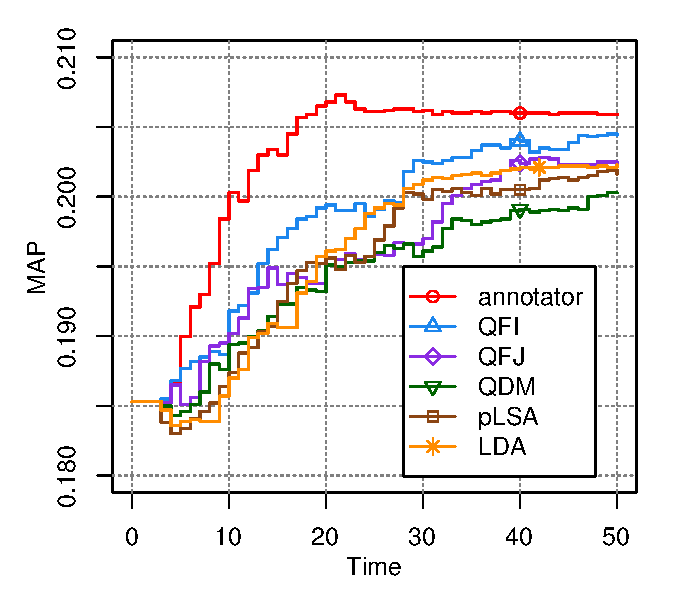
\epsfig{file=figure/cmp-facet-annotator-ffs-MAP.eps,scale=0.8}
\end{figure}

First, Figure~\ref{fig:cmp-facet} shows all models are able to improve ranking from the baseline, which testifies to the potential of FWS. However, the automatically generated facets are less effective than annotator facets. MAP for annotator facets reaches 0.2 by 10 time units, while the models need much more time, ranging from 27 to 47. Second, QFI is more effective than other models over the entire time span. This is consistent with the intrinsic evaluation. Third, the comparison results for other models are less clear. QFJ and QDM are better than pLSA and LDA before 20 time units, but MAP for pLSA and LDA increases much faster afterwards, and ends at a value similar to QFJ. Comparing these results with Table~\ref{tab:intrinsic}, we find intrinsic metrics do not always reflect utility based on extrinsic evaluation, though the generally better performance of QFI is clear in both.

Another way to compare is to see how many terms in the presented facets are selected by annotators, as shown in Figure~\ref{fig:cmp-facet-term}.
\begin{figure}[H]
\centering
\epsfig{file=figure/cmp-facet-annotator-term.eps,scale=0.8}
\caption{Number of feedback terms selected over time on facets generated by different models, based on annotator feedback.}
\label{fig:cmp-facet-term}
\end{figure}
The figure shows that with annotator facets a (simulated) user needs less time for selecting feedback terms. All the other facet generation approaches are similar to each other, with QDM having slightly more feedback terms at the beginning and QFI having more for the rest. This explains why QFI is the best system run in Figure~\ref{fig:cmp-facet-term} -- for the same time cost, QFI has more feedback terms selected by annotators.

If we switch to using the oracle feedback facets, the difference between different facet generation models and annotator facets are no longer that big, as shown in Figure~\ref{fig:cmp-facet-oracle}. Annotator facets are better at the beginning, but the corresponding MAP stops growing at around 20 time units. We find this is due to there not being so many facets available in the annotator facets. The number of terms and facets presented to users will affect this evaluation. In the plot, when there is not a sufficient supply of facets at some time cost, the results from a smaller time cost are used. That is, if the user runs out of facet terms to consider, performance is stuck where it last left off. 
\begin{figure}[H]
\centering
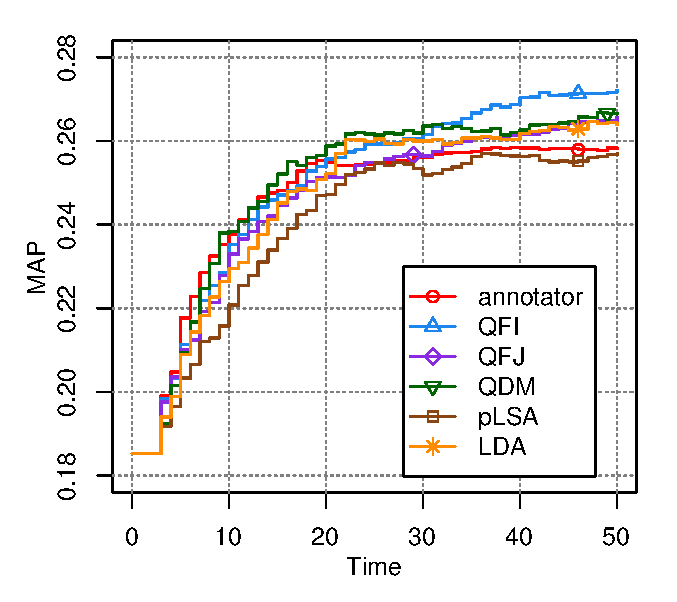
\epsfig{file=figure/cmp-facet-oracle-ffs-MAP.eps,scale=0.8}
\caption{MAP change over time for different facets generation models, based on oracle feedback and SF feedback model.}
\label{fig:cmp-facet-oracle}
\end{figure}

To validate the comparison in Figure~\ref{fig:cmp-facet} and~\ref{fig:cmp-facet-oracle}, we plot  Figure~\ref{fig:cmp-facet-cum-term} which shows the number of accumulated facet terms in the top facets generated by different models. Figure~\ref{fig:cmp-facet-cum-term} shows all models have a sufficient supply of facet terms for these evaluations. All of them present at least 50 facet terms (on average), which will need at least 50 time units for the user to process. This obviates the concern above. However, the annotator only has on average 42.3 facet terms selected, and therefore comparison at a time larger than that might unfairly penalize the annotator facets. We also notice that the first facet in QFI is very large, and overall QFI has more terms in top facets. Since the results are tuned on wPRF with equal weight for term precision and recall, this suggests it is very likely that too much weight is assigned for recall, and a more balanced weight between wP, wR and wFP should be used in wPRF.

%systems that provide giving more facets/terms will be more likely to have higher score when the allowed time is large. However, this will not affect the comparison when the time is small, or when the systems all present facets that could use that much time.
\begin{figure}[H]
\centering
\caption{Accumulated number of facet terms in top facets generated from different facets generation models.}
\label{fig:cmp-facet-cum-term}
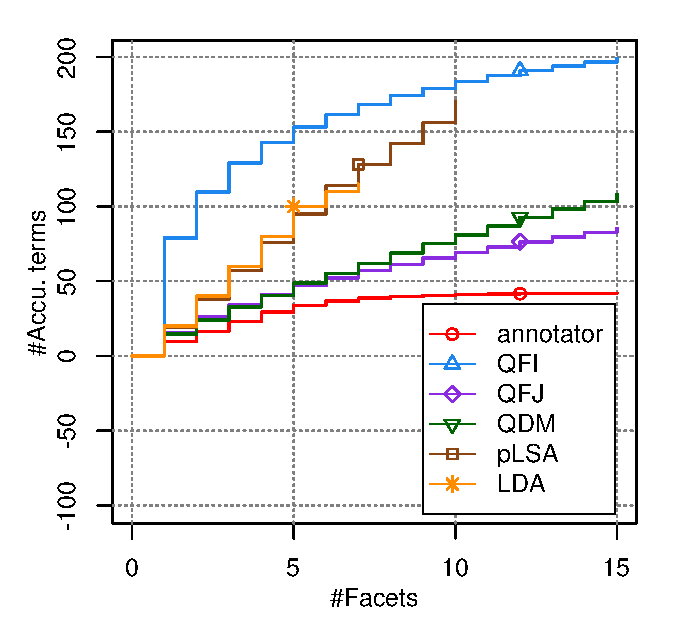
\epsfig{file=figure/cmp-facet-cumTerm.eps,scale=0.8}
\end{figure}

\subsection{Comparing Facet Feedback Models}
We compare different facet feedback models in Figure~\ref{sec:cmp-exp-model}. It shows soft ranking models are more effective than Boolean filter models. AND is too aggressive, which hurts the ranking performance as more and more feedback terms are used. The other two Boolean filtering models, OR and A+O, are similar at the beginning. That is because in the beginning there is only one feedback facet, in which case OR and A+O will be equivalent. As more facet terms are selected, A+O performance decreases. For the two soft ranking model, SF and ST are very close, with SF slightly better as time progresses. 
\begin{figure}[H]
\centering
\epsfig{file=figure/cmp-expansion-annotator-annotator-MAP.eps,scale=0.8}
\caption{MAP change over time for different feedback models, based on annotator facets and annotator feedback.}
\label{sec:cmp-exp-model}
\end{figure}
This comparison suggests that Boolean filter models, AND and A+O, are too strict for FWS, and a soft ranking model is more effective for FWS. This situation is probably because in FWS the mapping between facet term and document is incomplete; a document that does not contain the exact facet term may also be relevant. 



\subsection{Examples}
In this section, we use some system generated facets as examples, to show how FWS can assist search. We find FWS can be helpful in exploratory search. 
For example, for the query ``cheap internet'', the facets generated by QDM includes a facet of different Internet service types, \{\textit{dial up}, \textit{dsl}, \textit{cable}\}, and a facet of different ISPs, \{\textit{netzero}, \textit{juno}, \textit{copper}, \textit{toast}\}. These facets can assist the user to compare different Internet service types and ISPs during his/her exploration of ``cheap Internet''. Another example is the query ``lymphoma in dogs'', in which the user may want to learn about different aspects of lymphoma in dogs. QFJ generates the facet \{\textit{treatment}, \textit{diagnosis}, \textit{prognosis}, \textit{symptoms}, ...\} which represents different aspects of the query. For this query, there is a query subtopic looking for symptoms of lymphoma in dogs, which can be directly answered by another facet found by QFJ, \{\textit{vomiting}, \textit{diarrhea}, \textit{weight loss}, \textit{depression}, \textit{fever}\}. 


\section{Summary} 
\label{sec:ee-conclusions}
In this chapter, we developed an extrinsic evaluation method for Faceted Web Search. The extrinsic evaluation method directly measures the utility in search instead of comparing system/annotator facets as in intrinsic evaluation. We described a way to build reusable test collection for the extrinsic evaluation, and make our collected data set publicly available\footnote{See http://ciir.cs.umass.edu/downloads}.

We also investigated different facet generation and facet feedback models based on the extrinsic evaluation method.
Our experiments show, by using facet feedback from users, Faceted Web Search is able to assist the search task and significantly improve ranking performance.
Comparing intrinsic evaluation and extrinsic evaluation on different facet generation models, we find that the intrinsic evaluation does not always reflect system utility in real application. Comparing different facet feedback models, we find that the Boolean filtering models, which are widely used in conventional faceted search, are too strict in Faceted Web Search, and less effective than soft ranking models.

%\chapter{Adaptive Query Facet Generation} \label{ch:anticipated}
In this chapter, we propose adaptive query facet generation as our anticipated work.

\section{Variety in Facet-Appropriateness}
During our study, we find that queries are often of different ``facet-appropriateness''. Here, we use ``facet-appropriate'' (or ``high facet-appropriateness'') to describe that a query is easy to generate facets for, or it tends to have many useful facets or facet terms. We find that some queries are naturally easier than others to generate high-quality query facets for. For example, queries about products, such as ``toilet'' and ``volvo'', tend to have more high-quality candidate lists extracted from search results, and are therefore easier than other complex queries, such as ``self motivation''.
Some queries tend to have more useful query facets than others.
Table~\ref{fig:nfacets} shows the distribution of the number of facets (from annotators) each query has, for the 196 queries we used in Section~\ref{sec:ee-exp}. We can see that the number of facets varies widely for different queries. The most facet-appropriate query has 27 facets, while the least facet-appropriate query has only one.
Similarly, some facets tend to have more important facet terms than others.
For example, the facet for flight types only contains two facet terms (``international'' and ``domestic''), while the facet for different airlines contains many more facet terms (e.g, AA, Delta, JetBlue, United).
\begin{figure}[ht!]
\centering
\epsfig{file=figure/number-facet.eps,scale=0.6}
\caption{Distribution on number of facets each query have}
\label{fig:nfacets}
\end{figure}


However, existing query facet generation models (described in Chapter~\ref{ch:facet}) do not capture the variety in facet-appropriateness of different queries. The topic modeling approaches (pLSA and LDA) return a fixed number of facets and facet terms for all queries. Similarly, QF-I/QF-J and QDMiner return the top K requested facets for all queries.
All these static approaches suffer from the problems that: 1) when the query is of high facet-appropriateness, they may miss many high-quality facets; 2) more importantly, when the query is of low facet-appropriateness, they may return many low-quality facets, which are extremely bad for user experience. 

\section{Adaptive Models}
In order to address the problems of facet-appropriateness variety, we propose adaptive query facet generation to suggest and rank the right number of query facets and facet terms for each queries, under a limited display space allocation. This can improve query facet generation and make it more practical. More specifically, when encountering complex and difficult queries (e.g., ``self motivation''), adaptive query facet generation will only suggest query facets of high confidence (or will even not suggest any query facets). This will avoid noisy results which may largely hurt user experience. Similarly, for other queries of low facet-appropriateness, adaptive query facet generation could avoid suggesting low-quality facets; for queries of high facet-appropriateness, it will include more high-quality facets in the results. In addition, the limited display space constraint in adaptive query facet generation also makes the setting more realistic for mobile environment in particular.

We will investigate different classification or ranking models for deciding whether to suggest a particular generated facet and facet term. We will need to design facet and facet term features to characterize the quality of the facet (as a whole) and facet term (within the its facet). These features can be based on item and item pair features designed for query facet generation (see Section~\ref{sec:facet-features}). We can also design new features based on the probabilities (of an item being a facet term and two facet terms being in the same facet) learned in QF-I/QF-J. We may also design other new features based on external resources, such as query logs and human created taxonomies (e.g., Freebase). These supervised models are promising, because they could take advantage of available human labels to learn whether or not to suggest a particular generated query facet (and a particular facet term).

\section{Evaluation}
We will also extend our intrinsic and extrinsic evaluation for adaptive query facet generation. A problem with the existing intrinsic and extrinsic evaluation is that they may not have enough penalty for low-quality facets and facet terms.
For intrinsic evaluation, in Section~\ref{sec:ee-cmp-facet-extrinsic}, we find that QF-I tends to have large sized facets, when tuned on wPRF with equal weight for term precision and recall. This suggests that too much weight is assigned for recall. Therefore, we plan to investigate a more balanced weight for wP, wR and wFP in wPRF, to avoid generating too many low-quality facets or facet terms. For extrinsic evaluation, our user model for estimating user feedback time assumes that users take the same amount of time for scanning different query facets. However, in reality, users may take much more time to examine facets and select facet terms for low-quality facets. Therefore, we plan to incorporate the factor of facet quality into the user model for estimating user feedback time.
 
%\chapter{Research Plan}
In this last part of the proposal, we outline the research plan for the anticipated work proposed in Chapter~\ref{ch:anticipated} and other dissertation related work as follows.

\begin{itemize}
 \item 04/2015-05/2015: Adaptive facet generation models. We will develop adaptive models to suggest and rank the right number of query facets and facet terms for queries of different ``facet-appropriateness'', under a limited display space allocation. We will investigate different classification or ranking models and design related features for deciding whether to suggest a particular generated facet and facet term.
 \item 05/2015-06/2015: Adaptive facet generation evaluations. We will extend our intrinsic and extrinsic evaluation for adaptive query facet generation. We plan to investigate a more balanced weight for wP, wR and wFP in wPRF, and incorporate the factor of facet quality into the user model to better estimate user feedback time.
 \item 07/2015-11/2015: Ph.D dissertation preparation and defense.
\end{itemize}

\chapter{Conclusions and Future Work}
\label{ch:conclusions}
\section{Conclusions}
In this thesis, we investigated Faceted Web Search, an extension of faceted search to the open-domain web setting. We studied three fundamental problems in Faceted Web Search, namely (1) how to automatically generate facets, (2) how to re-organize search results with user feedback on facets and (3) how to evaluate generated facets and entire systems. To address these problems, we have: (1) developed query facet extraction for automatic facet generation; (2) developed an intrinsic evaluation method for evaluating generated facets; (3) developed an empirical utility maximization approach and a selective query faceting method for improving query facet extraction in precision-oriented scenarios; (4) investigated both Boolean filtering and soft ranking models for facet feedback; (5) developed an extrinsic evaluation method that evaluates entire systems in terms of their utility and cost in assisting search.

In Chapter~\ref{ch:facet}, we developed query facet extraction, which extracts facets for a given query from its search results. Changing from a global approach that generates facets in advance for an entire corpus~\cite{stoica2007automating,dakka2008automatic} to a query-based approach, query facet extraction provides a promising direction for solving facet generation in Faceted Web Search.
By focusing on the search results, query facet extraction avoids dealing with the entire web, which is large and heterogeneous. By directly generating facets for queries, it also addresses the facet recommendation problem at the same time.
 
For query facet extraction, we developed a supervised approach based on a graphical model to recognize query facets from the noisy candidates found. The graphical model learns how likely a candidate term is to be a facet term as well as how likely two terms are to be grouped together in a query facet, and captures the dependencies between the two factors. We proposed two algorithms (\QFI and \QFJ) for approximate inference on the graphical model since exact inference is intractable. Compared with other existing methods, our models can easily incorporate a rich set of features, and learn from available labeled data.

In Chapter~\ref{ch:intrinsiceval}, we developed an intrinsic evaluation method that evaluates generated facets by comparing them with human-created ones. We described how to collect human annotations for query facets by a pooling method. We designed \PRF, an evaluation measure that combines precision and recall of facet terms with grouping quality, using weighted harmonic mean. The measure can adjust emphasis between the three factors for different application scenarios. Experimental results based on this intrinsic evaluation show that our supervised methods (\QFI and \QFJ), can take advantage of a richer set of features and outperforms other unsupervised methods. Our feature analysis based on this evaluation suggests several informative features for query facet extraction, including \textit{ContextListSim}, \textit{ListTermFreq.ListIDF}, \textit{ContextTextSim} and \textit{ListTextSiteFreq}. Our analysis on the candidate extraction patterns shows that the lexical pattern, UL pattern and SELECT pattern are more important than other patterns.

In Chapter~\ref{ch:precision}, we investigated query facet extraction models under precision-oriented scenarios, and improved our models in such scenarios. The precision-oriented scenarios consider a more practical setting, in which users care more about precision of presented facets than recall. From the investigation, we found that our model (\QFJ), optimized based on likelihood, fails to adapt to the precision oriented scenarios, suggesting likelihood could be loosely related to the performance measure in such scenarios. Thus, we developed an empirical utility maximization approach to optimize the performance measure instead of likelihood. However, exact optimization on the performance measure is difficult due to the non-continuous and non-differentiable nature of the objective. We solved this problem by approximating the performance measure using its expectation. Our experiments show that this empirical utility maximization approach significantly improves our query facet model (\QFJ) under precision-
oriented scenarios, suggesting utility is a better learning objective than likelihood, and our expectation-based approximation is effective. 
 
Besides empirical utility maximization, we also improved query facet extraction performance in the precision-oriented scenarios by selective query faceting. In our investigation, We found query facet extraction quality varies drastically from excellent to poor and completely noisy. In the precision-oriented scenario, it may be more desirable to avoid showing facets for those poor performing queries and leave the users with a clean keyword-search interface. Thus, we proposed selective query faceting to show facets for good performing queries and avoid poor performing ones. A key problem, however, is how to predict the extraction performance. To solve the problem, we proposed a PRF score based on the expectation of \PRF to predict the performance. We show this score has fairly good prediction performance which enables selective query faceting, and improves the performance for the selected queries with fair coverage over the entire query traffic.

In Chapter~\ref{ch:feedback}, we investigated both Boolean filtering and soft ranking models for facet feedback. The Boolean filtering models filter the search results based on users' selection on facets, which is the dominant feedback model in conventional faceted search. Instead, soft ranking models re-ranks the documents by expanding the original query with selected terms in facets. Our experiments (in Chapter~\ref{ch:extrinsiceval}) show that the Boolean filtering models are too strict in Faceted Web Search, and less effective than soft ranking models.

In Chapter~\ref{ch:extrinsiceval}, we developed our extrinsic evaluation method that evaluates entire Faceted Web Search systems in terms of their utility in assisting search in an interactive search task. In the search task, a user searches an under-specified query, the FWS system provides query facets from which the user can select terms in the facets that would help further specified the query, after which the FWS system uses the feedback terms for re-ranking documents. Our extrinsic evaluation considers both gain in terms of the re-ranking performance and cost in terms of the time users spend for selecting feedback terms. The re-ranking gain can be measured by standard IR metrics like MAP or nDCG. The time cost ideally can be exactly measured by carrying out user studies. 

However, we noticed the user-study-based time measurement would make the evaluation difficult and expensive to extend for evaluating new systems rapidly. Thus, we proposed to simulate the user feedback process based on a user interaction model, using oracle feedback terms and feedback terms collected from human annotators. Both the oracle feedback and annotator feedback incrementally select all feedback terms that a user may select, which will then be used in simulation based on the user model to determine which subset of facet terms are selected by a user and how much time is spent giving that feedback. We also describe a way to build reusable test collection for the extrinsic evaluation, and make our collected data set publicly available\footnote{See http://ciir.cs.umass.edu/downloads}.

Our experiments show, by using facet feedback from human annotator, Faceted Web Search is able to assist the search task and significantly improve ranking performance if allowed sufficient time for user feedback: 18.0\% in NDCG@10 if we allow users to examine 50 terms in facets, and 7.4\% in NDCG@10 if we allow time for examining 10 terms. Our experiments also show that the skip list structure in the facet interface helps users save time in considering feedback terms in irrelevant facets. Comparing intrinsic evaluation and extrinsic evaluation on different facet generation models, we found that the intrinsic evaluation does not always reflect system utility in real application. Comparing different facet feedback models, as mentioned earlier, we found that the Boolean filtering models are too strict in Faceted Web Search, and less effective than soft ranking models.

\section{Future Work}
As a first extensive attempt at extending faceted search to the open-domain web, this work has some limitations, but also opens up many interesting directions for future work.


% query facet with labels, or high-level taxonomies as two or more level taxonomies in
In this work, a query facet is defined as a set of coordinate terms (\eg, \{\concept{AA}, \concept{JetBlue}, \concept{Delta}\}), but with no label (\eg, \concept{airlines}) for the set . This facet representation corresponds to one-level faceted taxonomies, in which information objects that belong to a same parent node are shown as a facet. However, explicitly showing labels for each query facets, or equivalently showing two-level faceted taxonomies, would be more desirable, as facet labels could help users quickly comprehend each query facets. There are two potential directions for solving this facet labeling problem. First, we could resort to some extraction patterns that extract facet candidates together with their labels.
For example, from the sentence \concept{... \underline{airlines} such as AA, Delta, and JetBlue.}, based on the pattern ``\textit{\underline{NP}} such as \textit{NP}, \textit{NP}, ..., and \textit{NP}'', we can extract facet candidate \{\concept{AA}, \concept{Delta}, \concept{JetBlue}\} together with the label \concept{airlines}. After candidate extraction, we need models for refining candidate facets with labels, which is also a very interesting problem. Second, we can resort to existing taxonomies. We can classify extracted query facets in to the taxonomies (\eg, assign \concept{AA}, \concept{Delta}, \concept{JetBlue} as child nodes for the node \concept{airlines} in the taxonomy), and then use the assigned parent nodes as labels. One problem with this direction is that existing taxonomies will almost certainly have difficulties in covering all query facets web search users are interested in. 

% ranking facets
In Chapter~\ref{ch:facet}, we used a heuristic score for ranking extracted query facets. The score is defined as $score(F)=\sum_{t \in F}{P(t)}$, which sums up the probabilities of each term $t$ being facet term, in order to present more facet terms in top ranks. This ranking model might be far from optimal, and there are other ranking models that could potentially improve facet ranking performance. For example, learning-to-rank models~\cite{liu2009learning} have been well-studied, and according to their success in information retrieval, they may also work for query facet ranking. However, one problem with using learning to rank is that we need to design informative features that measures the quality of a extracted query facet.

% other resources for extracting query facets or features for improving extraction performance
In this work, we focused on extracting query facet from search results. However, a variety of other resources can be useful for query facet extraction. For example, existing taxonomies or knowledge bases (\eg, Freebase\footnote{www.freebase.com}) can be useful for extracting candidate facets. Ideally, we can identify concepts (or entities) in a taxonomy that are relevant to the query, and then use the concepts with their child nodes as facet candidates (or query facets directly). For example, if we find that the concept \concept{airline} is relevant to our query \concept{baggage allowance}, and the taxonomy contains a node for \concept{airline}, then we can use the concept's child nodes (\concept{AA}, \concept{Delta}, \concept{JetBlue}) as facet candidates. We can also design features based on taxonomies to improve our models, such as the feature \concept{if two terms are assigned to the same parent node in a taxonomy}. Besides taxonomies or knowledge bases, query logs can also be helpful. They can be used 
to extract 
features to measure how useful and important facet terms or query facets are, and potentially improve term ranking within query facets, or facet ranking. For example, there may be many airlines extracted in the airline facet, based on statistics in query logs, we can easily find which airlines are more popular and rank them ahead in the query facet.

% optimizing utility in inferencing
In Chapter~\ref{ch:precision}, to improve the performance in precision-oriented scenarios, we used an empirical utility maximization approach that optimizes the performance measure for training our query faceting models. However, we have not investigated  decision theoretic approaches, advocated by \citet{lewis1995evaluating}, which try to optimize the performance measure during inferencing. \citet{nan2012optimizing} compared both approaches for optimizing F-Measures. Their results suggest that the two approaches are asymptotically equivalent given large training and test sets. Nevertheless, their experiments show that the empirical utility maximization approach appears to be more robust against model misspecification, and given a good model, the decision-theoretic approach appears to be better for handling rare classes and a common domain adaptation scenario. It would be interesting to also develop decision theoretic approach for optimizing \PRF measure, and compare with our proposed empirical utility 
maximization 
approach.


% extrinsic evaluation user models
Lastly, in Chapter~\ref{ch:extrinsiceval}, we used a simple user interaction model based on some strong assumptions that may not hold in real scenarios. For example, in the user model, we originally model the time a user spends for scanning a facet $F$ as $T(F)$. However, to simplify the estimation, we assumed time costs are equal for scanning different facets (\ie, $T(F)=T_f$, where $T_f$ is a constant). In reality, the time a user spends scanning a facet is highly dependent on the facet quality. Users may spend much more time for low-quality facets, in order to figure out what the facets are about. For example, the extracted facet \{\concept{AA}, \concept{first}, \concept{Delta}, \concept{business}, \concept{JetBlue}\} mixes facet \concept{airline} and facet \concept{flight classes} together. When a user encounters this facet, he or she may be confused and take more time in scanning.
To improve time estimation, we could model the time cost based on the facet quality.











\backmatter  %% <--- mandatory


%%
%% A bibliography is required.
\interlinepenalty=10000  % prevent split bibliography entries
\bibliography{thesis}
\end{document}